\chapter{SMASH transport approach: implementation and testing}
\label{chap:smash}

This chapter is largely based on \cite{Weil:2016zrk}.
A significant part of the work on this thesis was devoted to developing
a new transport approach, SMASH (Simulating Many Accelerated
Strongly-interacting Hadrons), which is described in this chapter.
SMASH is used for an investigation carried out in chapter \ref{chap:forced_therm}.
Conceptually the approach is similar to UrQMD, which was used in chapters
\ref{chap:local_equilibration} and \ref{chap:cooper_frye}. The main
difference is that SMASH is a transport
approach of a BUU type, while UrQMD is of QMD type (see section \ref{sec:transport}
for BUU vs. QMD discussion). This difference mainly matters for the
treatment of potentials and in the studies of this thesis potentials are not
included. The reasons to use SMASH in the following investigation are rather
technical than physical: SMASH is developed from scratch under version control,
it is written in C++, it undergoes continuous testing (both from programming and
physics side) and the implementation of forced thermalization approach appeared to be
technically easier in SMASH. The current version of SMASH is 1.0rc, however the
studies in chapter \ref{chap:forced_therm} were performed with an earlier version
SMASH-0.9rc.

As a transport approach SMASH solves a coupled set of Boltzmann
equations (\ref{eq:boltzmann},\ref{eq:buu_icoll}) via the Monte-Carlo method with
the test-particle ansatz

\begin{equation}
  \mathit{f}(x,p) = \frac{1}{N_{test}} \sum \delta^{(3)}(x - x_i) \delta^{(3)}(p - p_i) \,.
\end{equation}

Here every physical particle is represented by $N_{test}$ testparticles,
which sample the distribution function. To simulate the left part of the BUU
equation (\ref{eq:boltzmann}) it is enough to propagate particles according to their
equations of motion. The collision integral (\ref{eq:buu_icoll}) is solved via
simulating particle collisions and decays.

The testparticle ansatz also requires that interaction cross-sections are
modified:

\begin{align}
  \label{eq:testparticles_method1}
  \sigma & \mapsto \sigma \cdot \Ntest^{-1} \\
  \label{eq:testparticles_method2}
  N & \mapsto N \cdot \Ntest
\end{align}

In this way the average scattering rate (number of collisions per unit time per
particle) remains unchanged. The testparticle ansatz has three effects.
Firstly, the more testparticles are used the more precisely the distribution function
$\mathit{f}(x,p)$ is sampled. Due to the geometrical treatment of cross-sections,
particles in SMASH can interact at non-zero distance in contrast to field
theory, where all the interactions are local. So, secondly, the larger $\Ntest$
the smaller are the non-locality effects introduced by the collision criterion.
Thirdly, as shown in \cite{Cheng:2001dz}, experimental observables such as particle
spectra and flow obtained using transport models depend on $\Ntest$ and saturate
when $\Ntest$ is sufficiently large (in case of \cite{Cheng:2001dz}
$\Ntest = 16$ was large enough for saturation).

\section{Degrees of freedom}

The degrees of freedom entering BUU equations in SMASH are hadrons and
strings. The number of coupled BUU equations coincides with the number of degrees
of freedom.

\subsection{Hadrons in SMASH}

All hadrons consisting of the light quarks listed in the Review
of Particle Properties \cite{Agashe:2014kda}, which have an experimental status
''***'' or ''****'', are taken into account in SMASH. This notation for status means
that the existence of these hadrons is experimentally confirmed with high reliability.

The classification of light quark hadrons by quark content using the
$\SUgroup{3}$ flavour group is shown in appendix \ref{sec:SU3}.
These hadrons and their total angular momentum and radial excitations
constitute the hadron spectrum in SMASH.

Currently SMASH has 46 unflavoured mesons, 12 mesons with open strangeness,
17 $N$ baryons, 8 $\Delta$ baryons, 14 $\Lambda$ baryons, 10 $\Sigma$ baryons,
6 $\Xi$ baryons and 2 $\Omega$ baryons. In this counting scheme the whole isospin group
is considered as one particle, for example proton and neutron are counted as one
baryon or the group $\Delta^{++}$, $\Delta^{+}$, $\Delta^{0}$ and $\Delta^{-}$ is
also counted as one $\Delta$ baryon. Antiparticles are also included.

All of these particles are unstable except the proton, but every combination of
 (anti-~)~quarks in a strong-interaction ground state lives long enough, so that in
our simulations it may be considered as stable. A particle is treated as
stable, if its width does not exceed 10 keV (such as the lightest $\pi$, $\eta$, $K$,
N, $\Lambda$, $\Sigma$, $\Xi$, $\Omega$).

Every particle is characterized by the following parameters taken from
experimental data \cite{Agashe:2014kda}: the pole mass, the width at the pole mass,
quantum numbers, decay channels and branching ratios. Branching ratios are assumed to
be independent of mass.

\subsection{Hadron spectral function} \label{sec:spectral_function}

Every unstable hadron is characterized by a spectral function $\mathcal{A}(m^2)$ -
the probability to find it in a state with mass $m$, given that it has
pole mass $M_0$. In SMASH this is implemented by sampling the mass $m$
from the spectral function, when the resonance is produced. The particular
form of $\mathcal{A}(m^2)$ used in SMASH, called relativistic Breit-Wigner function,
can be understood from the following considerations.

The quantum field theory propagator of the particle, including interactions can be
written according to Dyson-Schwinger equation as

\begin{equation}
  \mathcal{G}(p) = \frac{1}{\mathcal{G}_0^{-1}(p) + \Sigma(p)} \,,
\end{equation}

where $G_0(p)$ is the propagator of non-interacting particle and $\Sigma(p)$ is
the so-called self-energy containing quantum loop corrections to the propagator. For
the scalar field

\begin{equation}
  \mathcal{G}_0(p) = \frac{1}{p^{\mu}p_{\mu} - m_{bare}^2} \,,
\end{equation}

where $m_{bare}$ is the bare mass in Lagrangian. For the Lorentz group representations
different from scalars (spinors, vector particles, etc) the propagator is still
proportional to the propagator of the scalar field. Splitting the self-energy
$\Sigma(p)$ into real and imaginary part, one can rewrite the full propagator as

\begin{align}
  \mathcal{G}(p) = \frac{1}{p^{\mu}p_{\mu} - M_0^2 + i \Im{\Sigma(p)}} \\
  M_0^2 = m_{bare}^2 - \Re{\Sigma(p)}
\end{align}

Here $M_0$ is the physical pole mass with interaction correction. This is the
mass taken from experimental data. Now the time-dependent propagator is
the inverse Fourier transformation

\begin{equation} \label{eq:t_dep_propagator}
  \mathcal{G}(t,\vec{p}) = \int \frac{d p^0}{2\pi} e^{i p^0 t}
    \frac{1}{p^{\mu}p_{\mu} - m_0^2 + i \Im{\Sigma(p)}} \,.
\end{equation}

This expression can be interpreted to use in a transport code. The Monte-Carlo
interpretation of the integral in Eq. (\ref{eq:t_dep_propagator}) is the
following: instead of propagating an off-shell particle one can propagate an
on-shell particle with a mass chosen with probability

\begin{align}
  w(m) \sim |m^2 - m_0^2 + i \Gamma(m)|^{-2} \\
  \Gamma(m) = \Im{\Sigma(m)}
\end{align}

In general $\Sigma(p)$ depends on the medium surrounding the particle, which
leads to the off-shell equations of motion \cite{Cassing:2009vt}. However, in
SMASH these in-medium effects are neglected (the effects of accounting them are
discussed in \cite{Cassing:1999mh} and are usually small for hadronic observables).
Therefore all unstable particles
(``resonances'') are assumed to have the shape of a relativistic Breit-Wigner for the
spectral function, resulting in the probability of a resonance with mass $m$:

\begin{equation}
  \mathcal{A}(m^2) = \frac{\mathcal{N}}{\pi} \frac{m \Gamma(m)}{(m^2 - M_0^2)^2 + m^2 \Gamma(m)^2} \,,
\end{equation}

where $\mathcal{N}$ is a normalization factor chosen in such a way that

\begin{equation}
  \int\displaylimits_0^\infty \mathcal{A}(m^2)dm^2 =
  \int\displaylimits_{m_{\textrm min}}^\infty \mathcal{A}(m^2)dm^2 = 1
\end{equation}

\subsection{Resonance width} \label{sec:width}

The total width $\Gamma$ in the previous expression is not constant, but given by the
mass-dependent function $\Gamma(m)$. Each resonance has a minimum mass
$m_\text{min}$ corresponding to the sum of masses of the lightest decay channels,
below which the width, and thus also the spectral function, vanishes. The total width
is computed as the sum of all partial widths:

\begin{equation}
  \Gamma(m)=\sum_i \Gamma_i(m)
\end{equation}

The computation of the decay widths follows the formalism of Manley et
al.~\cite{Manley:1992yb}, where in general the width of a two-body decay
$R\rightarrow ab$ is written as

\begin{equation} \label{eq:off_shell_width}
  \Gamma_{R\rightarrow ab} = \Gamma^0_{R\rightarrow ab} \frac{\rho_{ab}(m)}{\rho_{ab}(M_0)}.
\end{equation}

Here $m$ is the actual off-shell mass of the resonance R, $M_0$ is its pole
mass, $\Gamma^0_{R\rightarrow ab}=\Gamma_{R\rightarrow ab}(M_0)$ is the partial
width at the pole mass and the function $\rho_{ab}$ is defined as

\begin{align} \label{eq:rho_definition}
  \rho_{ab}(m) = \int & dm^2_a dm^2_b \mathcal{A}_a(m^2_a)\mathcal{A}_b(m^2_b) \nonumber \\
               \times & \frac{p_{cm}}{m} B_L^2(p_{cm}R) \mathcal{F}_{ab}^2(m).
\end{align}

In this formula, $m_a$ and $m_b$ denote the (off-shell) masses of the particles
a and b (which are being integrated over), $\mathcal{A}_a$ and $\mathcal{A}_b$
are their spectral functions and $p_{cm}$ is the absolute value of the
final-state momentum of a and b in the center-of-mass frame, which is given by:

\begin{align} \label{eq:p_cm}
  \vec{p}_{cm}^{\,2}(m,m_a,m_b) = \frac{(m^2-(m_a+m_b)^2)(m^2-(m_a-m_b)^2)}{4m^2}
\end{align}

Finally, L is the orbital angular momentum of a and b in the final state and
$B_L$ are the so-called 'Blatt-Weisskopf functions' \cite{BlaWei}. The
parameter $R$ is usually called the 'interaction radius' and is assumed to have
a universal value of $R=1$ fm for all processes. The form factor
$\mathcal{F}_{ab}$ is only relevant for unstable decay products and will be
discussed further.

The simplest case is that of a resonance R decaying into two stable daughter
particles. Popular examples are $\Delta\rightarrow\pi N$ or
$\rho\rightarrow\pi\pi$. In this case, the daughters have fixed masses (i.e.
their spectral functions are just $\delta$ functions), so that the integrals
collapse:

\begin{equation}
  \rho_{ab}(m) = \frac{p_{cm}}{m} B_L^2(p_{cm} R)
\end{equation}

As an example, the width for the p-wave (L=1) decays of the $\rho$ and $\Delta$
(mentioned above) becomes

\begin{equation}
  \Gamma(m) = \Gamma_0 \frac{M_0}{m} \left|\frac{p_{cm}}{p_{cm,0}}\right|^3
              \frac{p_{cm,0}^{\,2}+\Lambda^2}{p_{cm}^{\,2}+\Lambda^2},
\end{equation}

using $B_1^2(x)=x^2/(1+x^2)$. Here $m$ and $M_0$ are the off-shell and pole
mass, respectively, while $p_{cm}$ and $p_{cm,0}$ denote the
final-state momenta in the center-of-mass frame for mass $m$ and $M_0$,
respectively. $\Lambda=1/R$ can be viewed as a cut-off parameter. For an s-wave
(L=0) decay like $\sigma\rightarrow\pi\pi$, the width simply becomes

\begin{equation}
  \Gamma(m) = \Gamma_0 \frac{M_0}{m} \frac{p_{cm}}{p_{cm,0}} \,,
\end{equation}

since $B_0^2=1$.

\begin{figure}
  \centering
  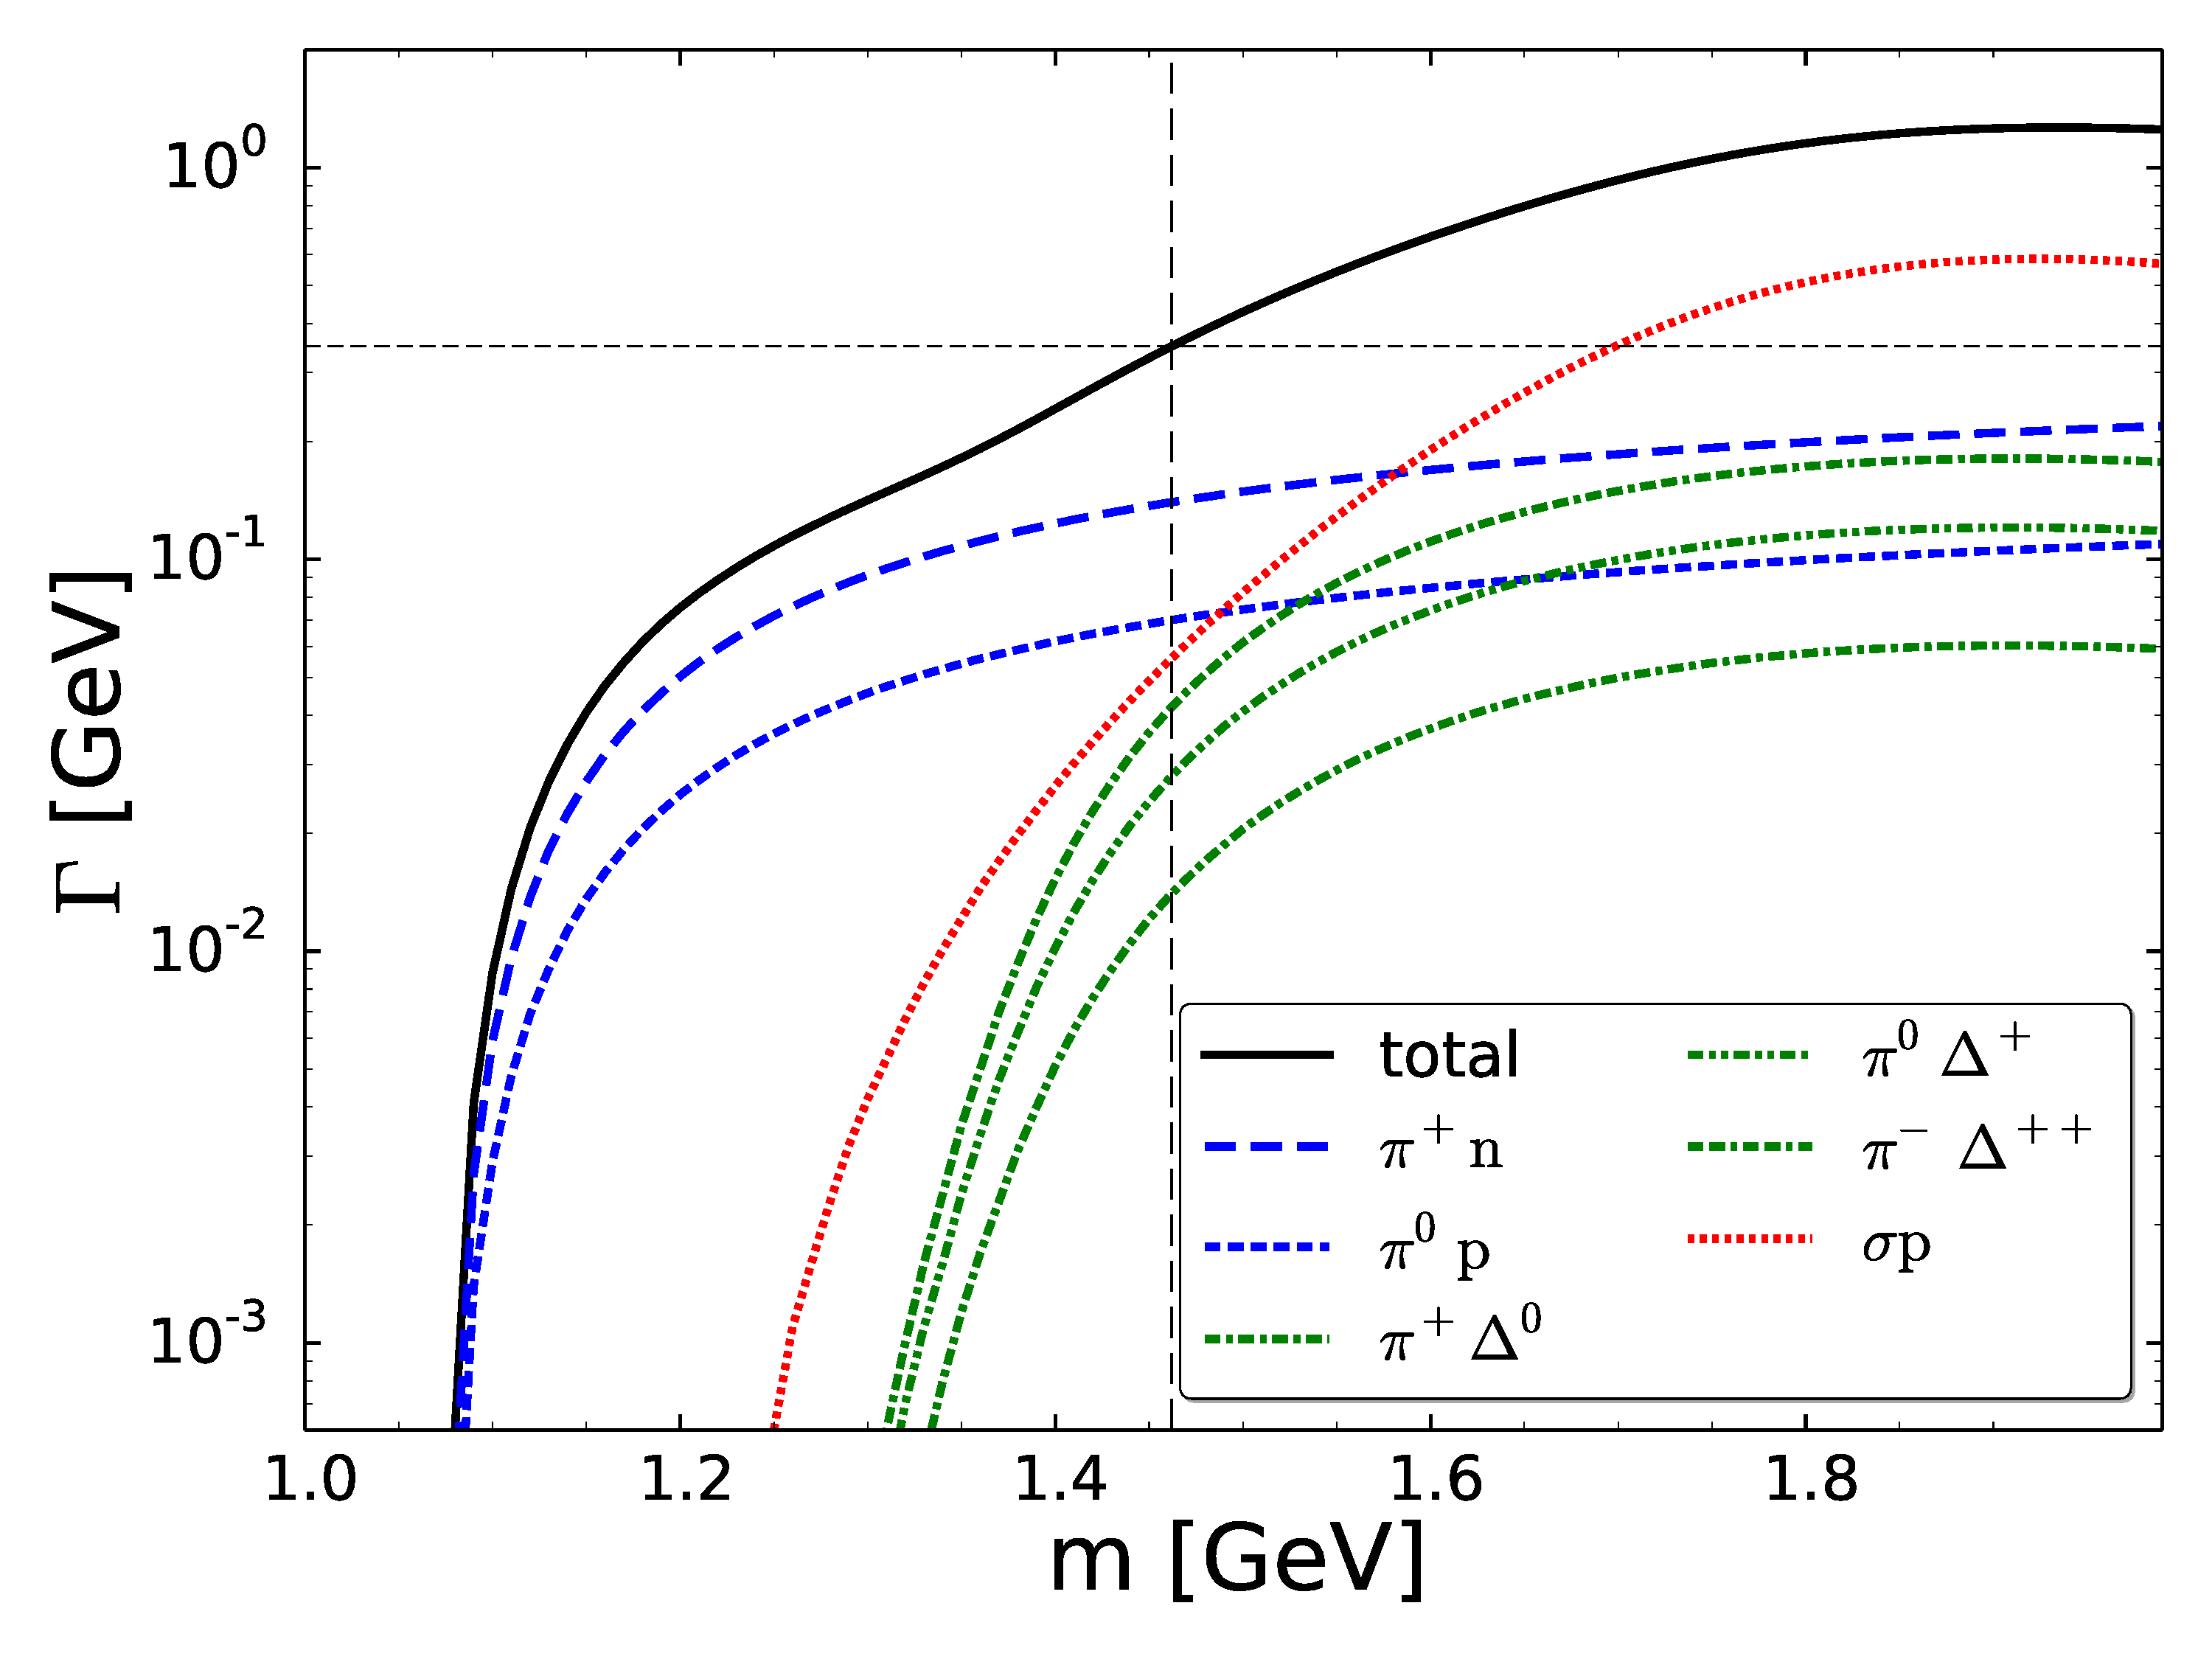
\includegraphics[width=0.8\textwidth]{plots/smash/width.pdf}
  \caption{Total and partial decay widths of the $N^*(1440)^+$ resonance
           as a function of mass. The vertical and horizontal dashed lines
           mark the pole mass and width.}
  \label{fig:width}
\end{figure}

In the case that one of the daughter particles is itself a resonance, the width
calculation becomes more difficult, since the mass of this daughter resonance
is not fixed and needs to be integrated over. Examples for this case are
$N^*(1440)\rightarrow\pi\Delta$ or $\omega\rightarrow\pi\rho$. As one of the
daughters is stable, at least one of the two integrals collapses:

\begin{equation} \label{eq:decay_semistable}
  \rho_{ab}(m) = \int \displaylimits_{m_a^{\textrm min}}^{m-m_b} dm^2_a
         \mathcal{A}_a(m^2_a) \frac{p_{cm}}{m} B_L^2(p_{cm} R)
         \mathcal{F}_{ab}^2(m)
\end{equation}

The remaining integral runs from the minimum allowed mass of particle a (i.e.
the threshold of its lightest decay channel) up to the maximum possible mass of
a in the decay process (given by $m-m_b$). The form factor $\mathcal{F}_{ab}$
(by M. Post \cite{Post:2003hu}) is used only if unstable decay products are
involved and is defined as

\begin{equation} \label{eq:post_ff}
  \mathcal{F}_{ab}(m) =
   \frac{\lambda^4+1/4(s_0-M_0^2)^2}{\lambda^4+\big(m^2-1/2(s_0+M_0^2)\big)^2},
\end{equation}

where the cut-off factors given in the table \ref{tab:cut-off} are used.

\begin{table}
\caption{Cut-off parameter $\lambda$ for form factor in resonance decay widths.}
\label{tab:cut-off}
\begin{tabular}{lc}
\toprule
 decay & $\lambda$ [GeV] \\
\midrule
 $\pi\rho$                                   & 0.8 \\
 unstable mesons (e.g. $\rho N$, $\sigma N$) & 1.6 \\
 unstable baryons (e.g. $\pi\Delta$)         & 2.0 \\
 two unstable daughters (e.g. $\rho\rho$)    & 0.6 \\
\bottomrule
\end{tabular}
\end{table}


It is easy to see that $\mathcal{F}_{ab}(M_0)=\mathcal{F}_{ab}(\sqrt{s_0})=1$.
Note that this form factor was not used by Manley originally, but was added
only later in the GiBUU implementation. The effect of the form factor is that
it suppresses the high-mass tail ($m>M_0$) and slightly enhances the low-mass
tail ($m<M_0$). Both of these effects get stronger with decreasing $\lambda$
($\mathcal{F}_{ab}\rightarrow 1$ for $\lambda\rightarrow\infty$). In this aspect
SMASH follows the GiBUU framework for the width parametrization of
resonances, since it has been proven to give a good description of experimental
data \cite{Buss:2011mx}.

To demonstrate the result of this formalism, in Fig. \ref{fig:width} the
theoretical decay width of the $N^*(1440)$ resonance is shown as a function of
mass. The total width is given as the sum of all partial widths. Each partial
width has a threshold that is given by the sum of the minimal masses of the
decay products. The branching ratios are fixed at the pole mass. One can see
that all partial widths increase as a function of mass, since more phase space
is available for heavier resonances. The lifetime correspondingly has an
opposite trend and heavy particles decay faster than low-mass resonances. Since
the width also enters in the production cross section, the
production of such low-mass resonances becomes more unlikely.

\subsection{Strings} \label{sec:strings}

At high $\sqrt{s}$ hadron collisions are not described by resonance excitations
anymore. In the regime of $\sqrt{s} \ge m_1 + m_2 + 2$ GeV, where $m_1$ and $m_2$
are masses of colliding particles, SMASH adopts Lund string model \cite{Andersson:1983ia}
to describe multiparticle production in the hadron-hadron collisions.
The used implementation of the Lund string model is PYTHIA 8 \cite{Sjostrand:2007gs}.
At the time, when the SMASH transport approach was applied for the studies relevant for
this thesis (see chapter \ref{chap:forced_therm}), strings were not yet implemented. 

\section{Initial conditions}

\subsection{Nucleus-nucleus collisions}

\paragraph{Nucleon Distribution in coordinate space}

\begin{table}
\caption{\label{tab:nuclei} Woods-Saxon initialization parameters for some nuclei.}
\begin{tabular}{lccc}
\toprule
Nucleus & $A$ & $r_0$ [fm] & $d$ [fm] \\
\midrule
U &  238 & 6.86 & 0.556  \\
Pb & 208 & 6.67 & 0.54 \\
Au & 197 & 6.38 & 0.535 \\
Cu & 63 & 4.20641 & 0.597  \\
\bottomrule
\end{tabular}
\end{table}

In SMASH a simple Woods-Saxon nucleon spatial distribution is implemented, as
 demonstrated in Fig. \ref{fig:woods-saxon}. The explicit form reads

\begin{equation} \label{eq:woods_saxon}
  \frac{dN}{d^3r} = \frac{\rho_0}{\expOf{\frac{r-r_0}{d}} + 1}
\end{equation}

where $r_0$ is the nuclear radius and $d$ is the diffusiveness, which controls
the quick fall-off of the distribution. For $d\rightarrow 0$, the nucleus would
be a hard sphere.  The ground state density $\rho_0 \approx 0.168$ fm$^{-3}$
emerges after $A$ nucleons are sampled.  The default value for the
diffusiveness is $d=0.545$ fm, where more specific values are used for Au, Pb,
Cu and  U (see Table \ref{tab:nuclei}).

\begin{figure}
  \centering
  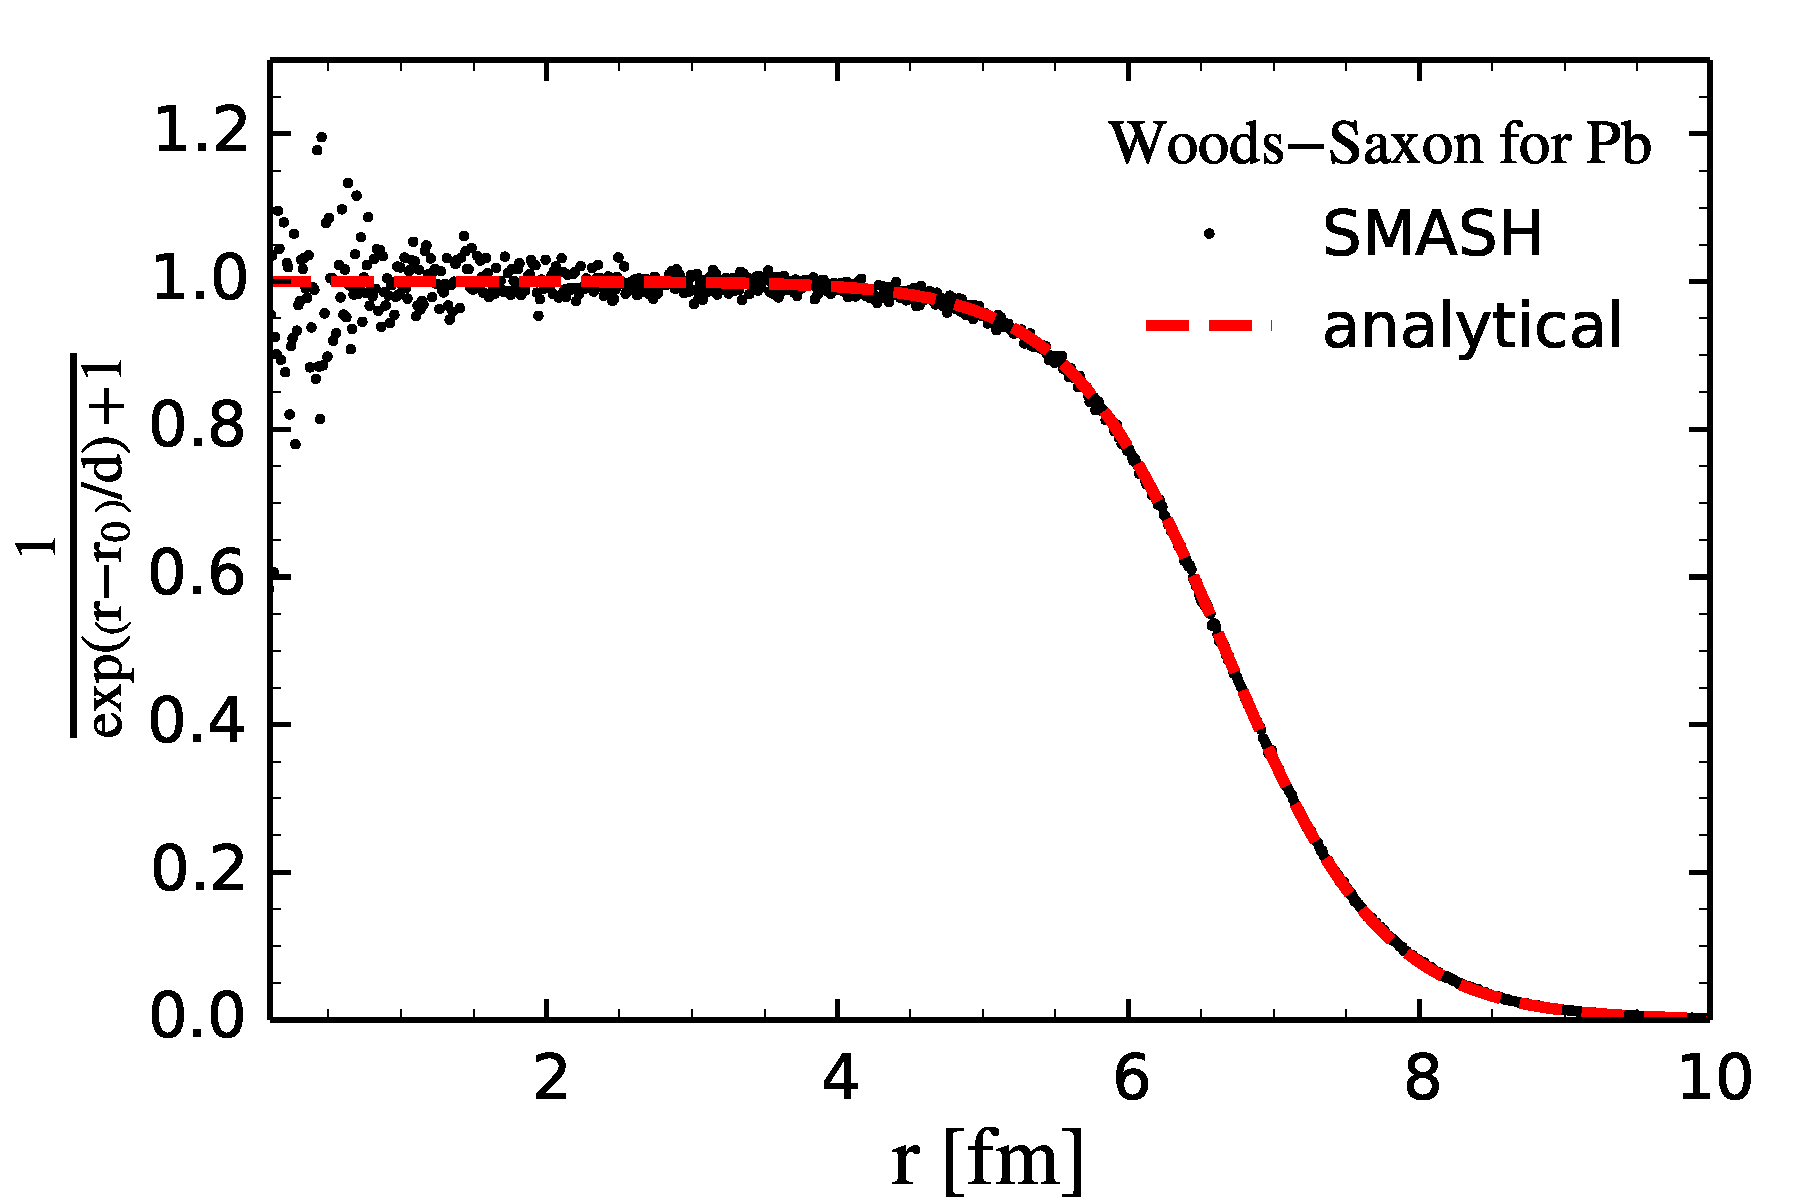
\includegraphics[width=0.8\textwidth]{plots/smash/woods_saxon_nor2.pdf}
  \caption{Sampled coordinate space distribution of 208 nucleons is compared to the
           Woods-Saxon distribution with the parameters for a lead nucleus.}
  \label{fig:woods-saxon}
\end{figure}

Within the sampling procedure nucleons are assumed to be independent.
The finite size of the nucleons and nucleon-nucleon correlations~\cite{Alvioli:2009ab}
are neglected for simplicity, as are the neutron skin effects~\cite{Tarbert:2013jze}.
Deviations from sphericity can optionally be taken into account up to the quadrupole
moment. No measures are taken to initialize the  nucleus in the ground state, like it
is done e.g. in~\cite{Gaitanos:2010fd}.

The initial positions of nuclei and the time of initialization are chosen as
shown in Fig. \ref{fig:init_coord_time}.  Cartesian coordinates are used, where the
$z$-direction corresponds to the beam direction and $x$ is the impact parameter
direction. At the initialization the projectile center is at $xz$-coordinates
$(b/2, - \Delta z- \gamma_P^{-1} (R_P + d_P))$ and the target center is at
$(-b/2, \frac{v_T}{v_P}\Delta z + \gamma_T^{-1} (R_T + d_T))$. Here $R_{P,T}$
are the projectile/target radii and $d_{P,T}$ are the corresponding
diffusiveness parameters from the Woods-Saxon distribution. By $v_{T,P}$ we
denote absolute values of the velocities, while  $\gamma_{P,T} = (1 -
v_{P,T}^2)^{-1/2}$ are the associated gamma-factors. The separation of the
centers of the nuclei in $x$-direction equals the impact parameter $b$. For
deformed nuclei an additional rotation along all three angles is applied. In
this way, the simulation is started at such an initial separation that the
potential of one nucleus does not influence the other one yet, otherwise
initialization in the ground state would not be justified.  The initial
coordinates and time are chosen in such a way that the Lorentz-contracted spheres
of radii $(R + d)_{P,T}$ will touch at $t = 0$ in a central collision. An
alternative definition would be that $t=0$ fm corresponds to the maximal
overlap of the two nuclei. The additional distance $\Delta z= 2$ fm is added to
avoid missing any nucleon-nucleon collisions. Since the nucleons are
distributed according to Woods-Saxon distributions, there is a small, but
non-zero probability to position a nucleon at a large distance from the nucleus
center. The initial separation distance $\Delta z$ is chosen such that all
collisions are taken into account. The initial time is $t_0 = \Delta z/v_P$,
which implies that the projectile is always moving, $v_P > 0$, while the target
can be at rest depending on the reference frame for the calculation.

\begin{figure}
  \centering
  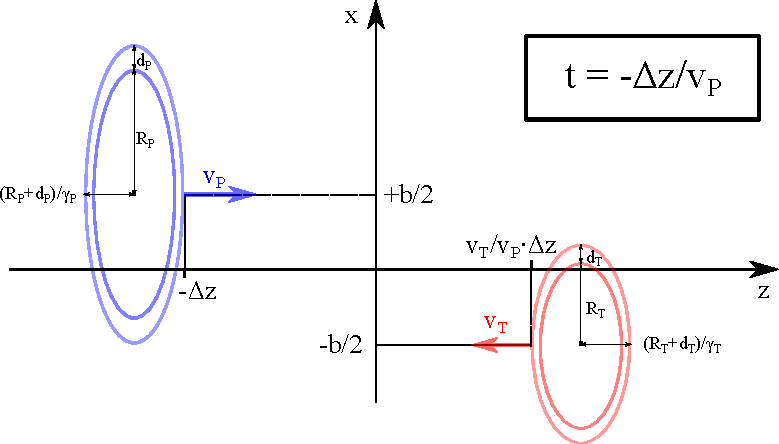
\includegraphics[width=0.8\textwidth]{plots/smash/AAcollision_SMASHt0convention.pdf}
  \caption{Initial positions of nuclei such that contracted spheres of radii
           $(R + d)_{P,T}$ will touch at $t = 0$ in a central collision.}
  \label{fig:init_coord_time}
\end{figure}

\paragraph{Fermi motion}

In momentum space nucleons optionally get Fermi momenta, then target and
projectile are boosted in $z$ direction according to the chosen energy of the
reaction and computational frame. The gamma-factor of the boost is $\gamma =
E_A/M_A$, where $E_A$ is the energy of the nucleus and $M_A$ is its mass. The
velocity of the boost is $\beta = p_A/E_A$. Note that in $E_A$ and $M_A$ one
has to account for the binding energy of the nucleus. For this an approximation used
in the JAM transport code~\cite{Nara:1999dz} is adopted, which assumes
that all nucleons are equally bound. Thus, the energy of each nucleon in the
rest frame of the nucleus is $E_i = M_A/A$, where $A$ is the number of
nucleons. With this assumption the boost of the longitudinal momenta $p'_{iz}$
to the computational frame becomes

\begin{align}
  p'_{iz} = \gamma (p_{iz} + \beta E_i) = \gamma p_{iz} + \frac{p_A}{M_A} \frac{M_A}{A} = p_\text{beam} + \gamma p_{iz} \,,
\end{align}

where $p_\text{beam}$ is the beam momentum per nucleon and $p_{iz}$ are the
momenta of nucleons in the rest frame of the nucleus. In our implementation
$p_\text{beam}$ and $\gamma$ themselves are computed without accounting for
binding energy. Note that there is no well-established procedure of boosting
nuclei accounting for their binding energy. Codes like UrQMD
\cite{Bass:1998ca}, JAM \cite{Nara:1999dz} and GiBUU \cite{Buss:2011mx}
apply different methods. Though the typical binding energy per nucleon is much
smaller than the nucleon mass $(\simeq 8 \text{ MeV}/938 \text{ MeV} \approx
1\%)$, the different methods of accounting for the binding energy
produce small but noticeable differences in pion multiplicities and mean
transverse momentum at low collision energies of $E_\text{kin} = 0.4-2A$ GeV.

The momentum distribution of nucleons in the ground state nucleus is generated
in the Local Density Approximation (LDA). At every spatial point the momentum
distribution is a uniformly filled Fermi sphere of radius

\begin{equation}
p_F (\vec{r}) = \hbar c (3 \pi^2 \rho (\vec{r}))^{1/3}
\end{equation}

Here $\rho(\vec{r})$ is the density of nucleons at the point $\vec{r}$.
A more detailed description of the density calculation is given in
section~\ref{sec:thermodynamics}. A typical value of $p_F \approx$ 300 MeV
corresponds to an energy of $p_F^2/(2m_N) \approx$ 45 MeV. The LDA
is probably the easiest and most naive choice to implement. A more realistic
treatment of Fermi motion includes Hartree-Fock mean-field calculation,
which justifies LDA in the range of momenta from 0.5 to 1 fm$^{-1}$ \cite{Jaminon:1986ktn}.
Similar conclusion can be made comparing Fig. \ref{fig:fermi} to experimentally
measured momentum distributions \cite{Gaidarov:1995pm}.

In LDA the momentum distribution of the nucleons can be computed analytically. In
the central part of the nucleus, where the density is almost constant, the momentum
distribution is just a Fermi sphere. This is indeed reproduced by SMASH, as shown in Fig.~\ref{fig:fermi}.
For the whole nucleus one has to properly average over the density:

\begin{align}
  \frac{dN}{p^2 dp} \sim \int \frac{dN(r)}{p^2 dp} d^3r \sim \int_0^{\infty} \theta(p_F(r)-p) \, r^2 dr = r^3_{max}(p)/3,\,
\end{align}

where $r_{max}$ is the root of the equation $p_F(r_{max})=p$. Let us find this root.

\begin{align}
  \left( \frac{p}{\hbar c}\right)^3 \frac{1}{3 \pi^2 \rho_0} = \frac{1}{1 + exp((r-R)/d)} \\
  (p_F^0/\hbar c)^3 = 3 \pi^2 \rho_0 \\
  r_{max}(p) = R + d \cdot \log \left(\left( \frac{p_F^0}{p} \right)^3 - 1 \right)
\end{align}

\begin{align}
  \frac{dN}{p^2 dp} \sim \left(1 +\frac{d}{R} \log[(p_F^0/p)^3 - 1] \right)^3 \, \theta(p_F^0 - p) \\
  \frac{dN}{dp^3} = A \left(1 +\frac{d}{R} \log[(p_F^0/p)^3 - 1] \right)^3 \, \theta(p_F^0 - p) \frac{1}{(p_F^0)^3} \,,
\end{align}

where $A$ is a dimensionless constant, which can be obtained from the normalization condition.
Let us rewrite the previous equation with $\xi = \left( \frac{p}{p_F^0} \right)^3$:

\begin{align}
  \frac{dN}{d\xi} = A \left(1 +\frac{d}{R} \log[\xi^{-1} - 1] \right)^3 \, \theta(1 - \xi)
\end{align}

Integration results in

\begin{align}
  \int_0^1 \left(1 +\frac{d}{R} \log[\xi^{-1} - 1] \right)^3 \, d\xi = 1 + \left( \frac{\pi d}{R} \right)^2 \\
  \frac{1}{N} \frac{dN}{d\xi} = \frac{1}{1 + \left( \frac{\pi d}{R} \right)^2} \left(1 +\frac{d}{R} \log[\xi^{-1} - 1] \right)^3 \, \theta(1 - \xi)
\end{align}


As Fig. \ref{fig:fermi} demonstrates, this theoretical expectation is matched by SMASH.

\begin{figure}
  \centering
  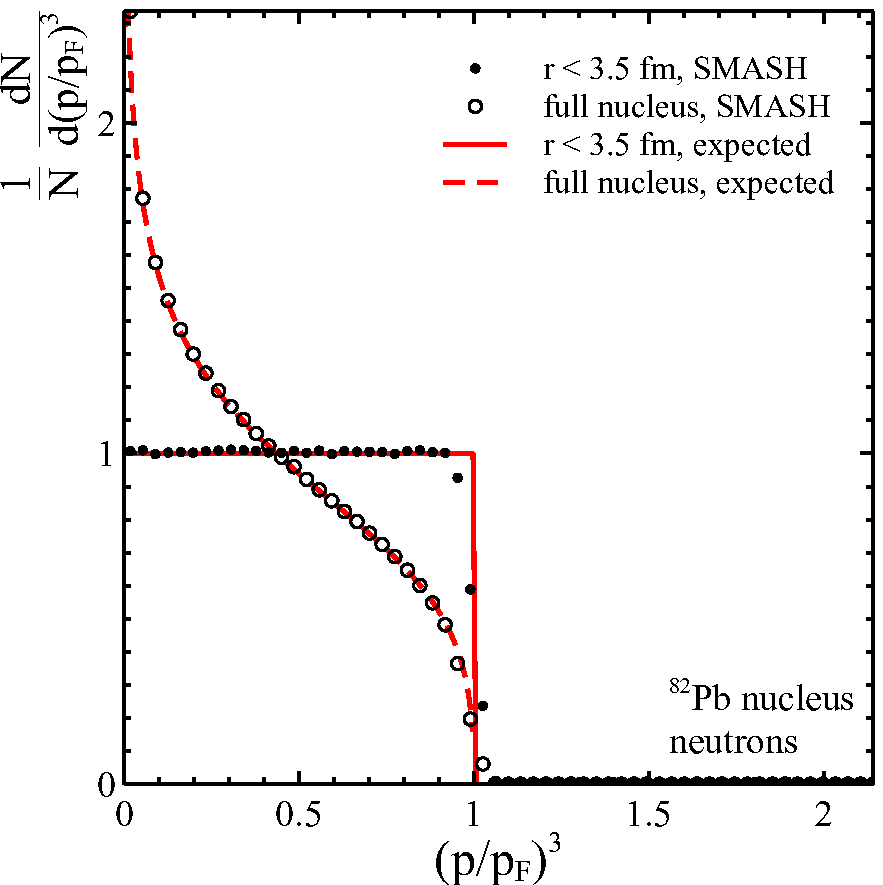
\includegraphics[width=0.6\textwidth]{plots/smash/Fermi_momenta_Pb.pdf}
  \caption{Momentum space distribution of neutrons compared to the analytical expectation for a lead nucleus. }
  \label{fig:fermi}
\end{figure}

Including Fermi motion is only sensible, if potentials are turned on
simultaneously. Otherwise, the nucleus will fly apart due to the finite
transverse momenta of the nucleons that need to be compensated by the
attractive mean field interaction. Alternatively, the so-called frozen Fermi
approximation can be be adopted, where the Fermi momenta are employed for the
collisions, but not for the propagation.

\subsection{Infinite matter (periodic box) calculations}

To simulate infinite hadronic matter or other simple systems like an ideal
massless or massive gas and investigate its thermodynamic properties, box
calculations are performed. There are two initialization options. Firstly, the
box can be initialized in the canonical ensemble with user-defined hadron
multiplicities $N_j$ of each hadron species. In this case $N_j$ does not change
from event to event. Secondly, multiplicities can be sampled from the Poisson
distribution

\begin{equation}
  N_{j} = Poi(n_j) \,,
\end{equation}

where $n_j(T, \mu_b, \mu_s)$ are the grand-canonical thermal multiplicities
given by Eq. (\ref{eq:hadgas_ni}). The coordinates of the $N$ particles $(x_j, y_j,
z_j)$ are sampled uniformly in the box. The momenta of the particles are
sampled from the isotropic thermal Boltzmann distribution with temperature $T$:

\begin{align}
    w(\vec{p}) &= \mathcal{N} \cdot \exp(-\sqrt{\vec{p}^{\,2} + m^2}/T) p^2 dp
                  \cdot \sin \theta d\theta d\varphi \; ,
\end{align}

where $w(p)$ is a probability to generate momentum $\vec{p}$, $\theta$ and
$\varphi$ are angles in spherical coordinates and $\mathcal{N}$ is a normalization
factor. Let us denote the total momentum of $N$ particles sampled from this
distribution $p_{\textrm tot}$. One can see that the ensemble average of $p_{\textrm
tot}$ is zero,

\begin{equation}
    \int \exp(-\sqrt{\vec{p}^{\,2} + m^2}/T) d^3p \cdot p_{x,y,z} = 0 \; ,
\end{equation}

because it involves an integral over an odd function. However, in each single
event $p_{\textrm tot} \neq 0$, which is corrected by changing the momentum of
every particle $p_j \to p_j - p_{\textrm tot}/N$. After this procedure the thermal
distribution is slightly spoiled, the total energy is changed and angle
uniformity is disturbed. This is a small effect for large numbers of particles, because
$\frac{p_{\textrm tot}}{E_{\textrm tot}} \sim \frac{1}{\sqrt{N}}$, where
$E_{\textrm tot}$ is the total energy of the particles. After letting the system
thermalize, the temperature differs by 1-2\% from the initialization temperature. One
also has to note that the total energy is not the same from event to event, it is
fluctuating, even without this momentum shift.

\section{Interactions}

\subsection{Collisions}

\subsubsection{Collision Criterion}

One of the challenges for solving the relativistic BUU equation is to define an
appropriate collision criterion. The Kodama criterion \cite{Kodama:1983yk} is a
fully covariant collision criterion, but since it involves boosts of several
four vectors it is rather inefficient.  In the SMASH approach the geometrical
criterion was chosen following the UrQMD (Ultra-relativistic Quantum Molecular
Dynamics) approach \cite{Bass:1998ca}. The geometrical criterion is defined as
follows:

\begin{equation} \label{eq:collision_criterion}
  d_{\textrm trans} < d_{\textrm int} = \sqrt{\frac{\sigma_{\textrm tot}}{\pi}}
\end{equation}

with

\begin{equation}
  d_{\textrm trans}^2 = (\vec{r_a}-\vec{r_b})^2 -
  \frac{((\vec{r_a}-\vec{r_b})\cdot(\vec{p_a}-\vec{p_b}))^2}{(\vec{p_a}-\vec{p_b})^2}
\end{equation}

where $\vec{r}$ and $\vec{p}$ are the coordinates and momenta of the two
particles $a$ and $b$ in the center of mass frame of the binary collision. The
time of the collision is determined as the time of the closest approach in the
computational frame:

\begin{equation} \label{eq:collision_time}
  t_{\textrm coll} = -\frac{(\vec{r_a}-\vec{r_b})\cdot (\vec{p_a}/E_a-\vec{p_b}/E_b)}
                       {(\vec{p_a}/E_a-\vec{p_b}/E_b)^2}
\end{equation}

where now all coordinate and momentum vectors have to be taken in the
computational frame. The computational frame is usually chosen to be the equal
velocity frame of the two nuclei, which is the same as the center of mass frame
in case of symmetric systems. The computational system is the one that carries
the clock that is relevant for ordering of the collisions, therefore it is
crucial to transform the collision times to the same frame to decide which
collision happens first.

An alternative option to include all relevant scatterings at high density is to
implement the solution of the Boltzmann equation by stochastic rates
\cite{Danielewicz:1991dh,Cassing:2001ds,Xu:2004mz}. This approach has the
advantage that multi-particle scatterings can be taken into account in a
straightforward way. On the hadronic level there are of course a lot of
different possibilities that one would need to take into account in such an
approach, therefore this is left for future work. Also, the stochastic rates
approach is relying on having a large number of test particles in each cell,
therefore it is not clear how to model event-by-event fluctuations properly.

\subsubsection{Elastic and inelastic reactions}

The elastic collisions can be truly elastic, where only momenta are exchanged
between the particles, and pseudoelastic, which proceed through a resonance
formations. In SMASH the meson-meson and baryon-meson reactions are assumed o be fully
determined by resonance excitation and decay,  e.g. $\pi N \to \Delta \to \pi N$
 or $\pi\pi \to \rho \to \pi\pi$. For baryon-baryon collisions on the other
hand the elastic cross sections are parametrized. The parametrizations of
the elastic pp and pn cross sections in particular are taken from
\cite{Weil:2013mya}, eq. (44) and (45).

Inelastic interaction in SMASH are $2 \leftrightarrow 2$ collisions
and $2 \to 1$ resonance formations. Many-particle reactions are not implemented,
but an effective way to account for them is discussed in
chapter~\ref{chap:forced_therm}. Cross-sections of resonance formation
are completely defined by the resonance properties and can be computed
from the detailed balance principle using Eq. \ref{eq:sigma_2to1}. The results of this
treatment for $\pi^+\pi^-$ and $\pi N$ cross-sections is demonstrated in Fig. \ref{fig:xs}.
One can see the a resonant structure of both cross-sections.

Three groups of $2 \to 2$ reactions are implemented:

\begin{enumerate}
  \item Single nucleon excitation reactions $NN\leftrightarrow NN$,
        $NN\leftrightarrow N\Delta$, $NN\leftrightarrow NN^*$ and $NN\leftrightarrow N\Delta^*$.
  \item Double nucleon excitation reactions $NN\leftrightarrow\Delta\Delta$,
        $NN\leftrightarrow\Delta N^*$ and $NN\leftrightarrow\Delta\Delta^*$.
        Here $N^*$ and $\Delta^*$ denote all possible excitations of nucleons
        and Delta-baryons.
  \item Strangeness exchange reactions $K^- N \leftrightarrow \pi Y$ with $Y = \Lambda, \Sigma$.
  \item $KN \leftrightarrow K\Delta$ and inelastic charge exchange $KN \leftrightarrow KN$
\end{enumerate}

For the process $NN\leftrightarrow N\Delta$, the parametrized energy dependence
is based on a fit to the Dmitriev one-boson-exchange (OBE) model
\cite{Dmitriev:1986st}. For $NN\rightarrow NR$ and $NN\rightarrow \Delta R$
with $R=N^*,\Delta^*$, the matrix element is assumed to be independent of
$s$, but can depend on the total isospin and the pole masses $m_a$ and $m_b$ of
the outgoing particles. The same is true for the parametrizations of double resonance
production $NN \to R_1 R_2$. For the parametrization details see\cite{Weil:2016zrk}.
The cross-sections are computed via Eq. \ref{eq:cs_forward22}, but additionally
isospin factors are taken into account. The reverse reactions cross-sections are
implemented via the detailed balance relations, see section \ref{sec:detbal_2to2}.
The resulting $NN$ total cross-section is demonstrated in Fig. \ref{fig:xs}.

For the strangeness exchange reactions the explicit experimental cross-section
parametrizations are taken from \cite{Graef:2014mra} and the reverse reactions
are implemented via detailed balance. The $KN \leftrightarrow K\Delta$ and
$KN \leftrightarrow KN$ cross-sections are also parametrized directly following
the GiBUU and using expressions from the Appendix A.2.4 of \cite{thesis_Effenberger}.

\begin{figure}
  \centering
  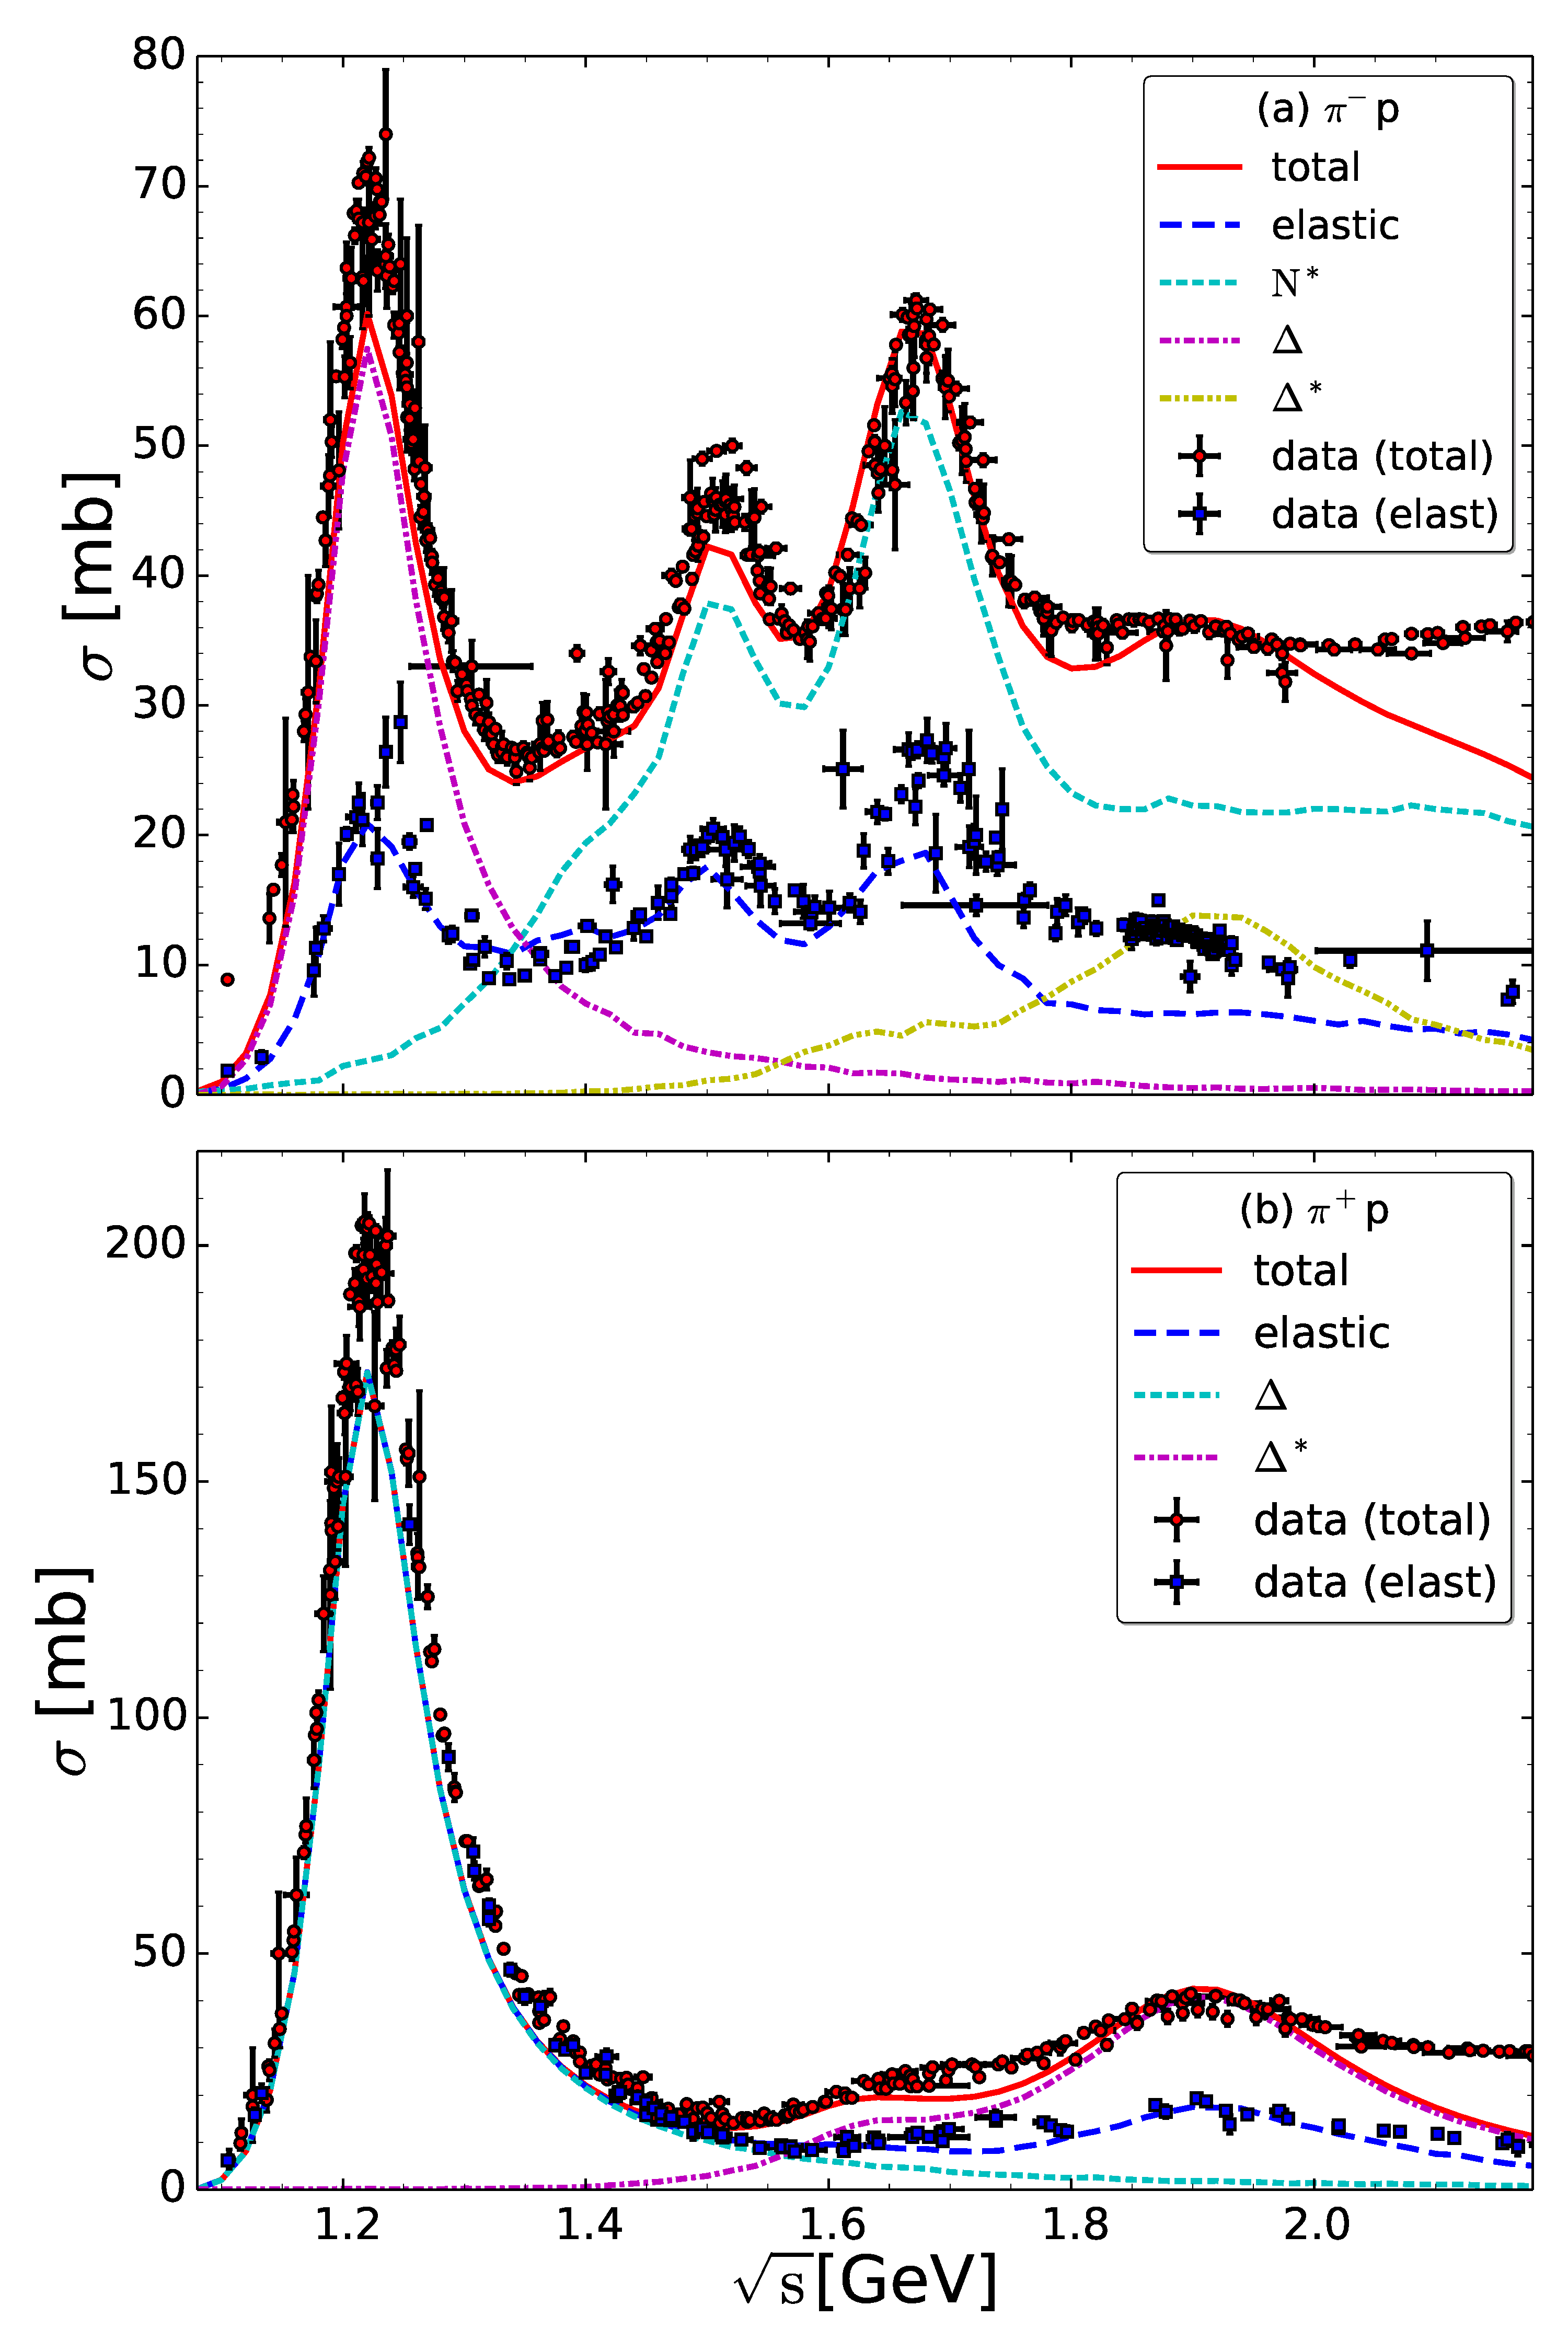
\includegraphics[width=0.49\textwidth]{plots/smash/piN.pdf}
  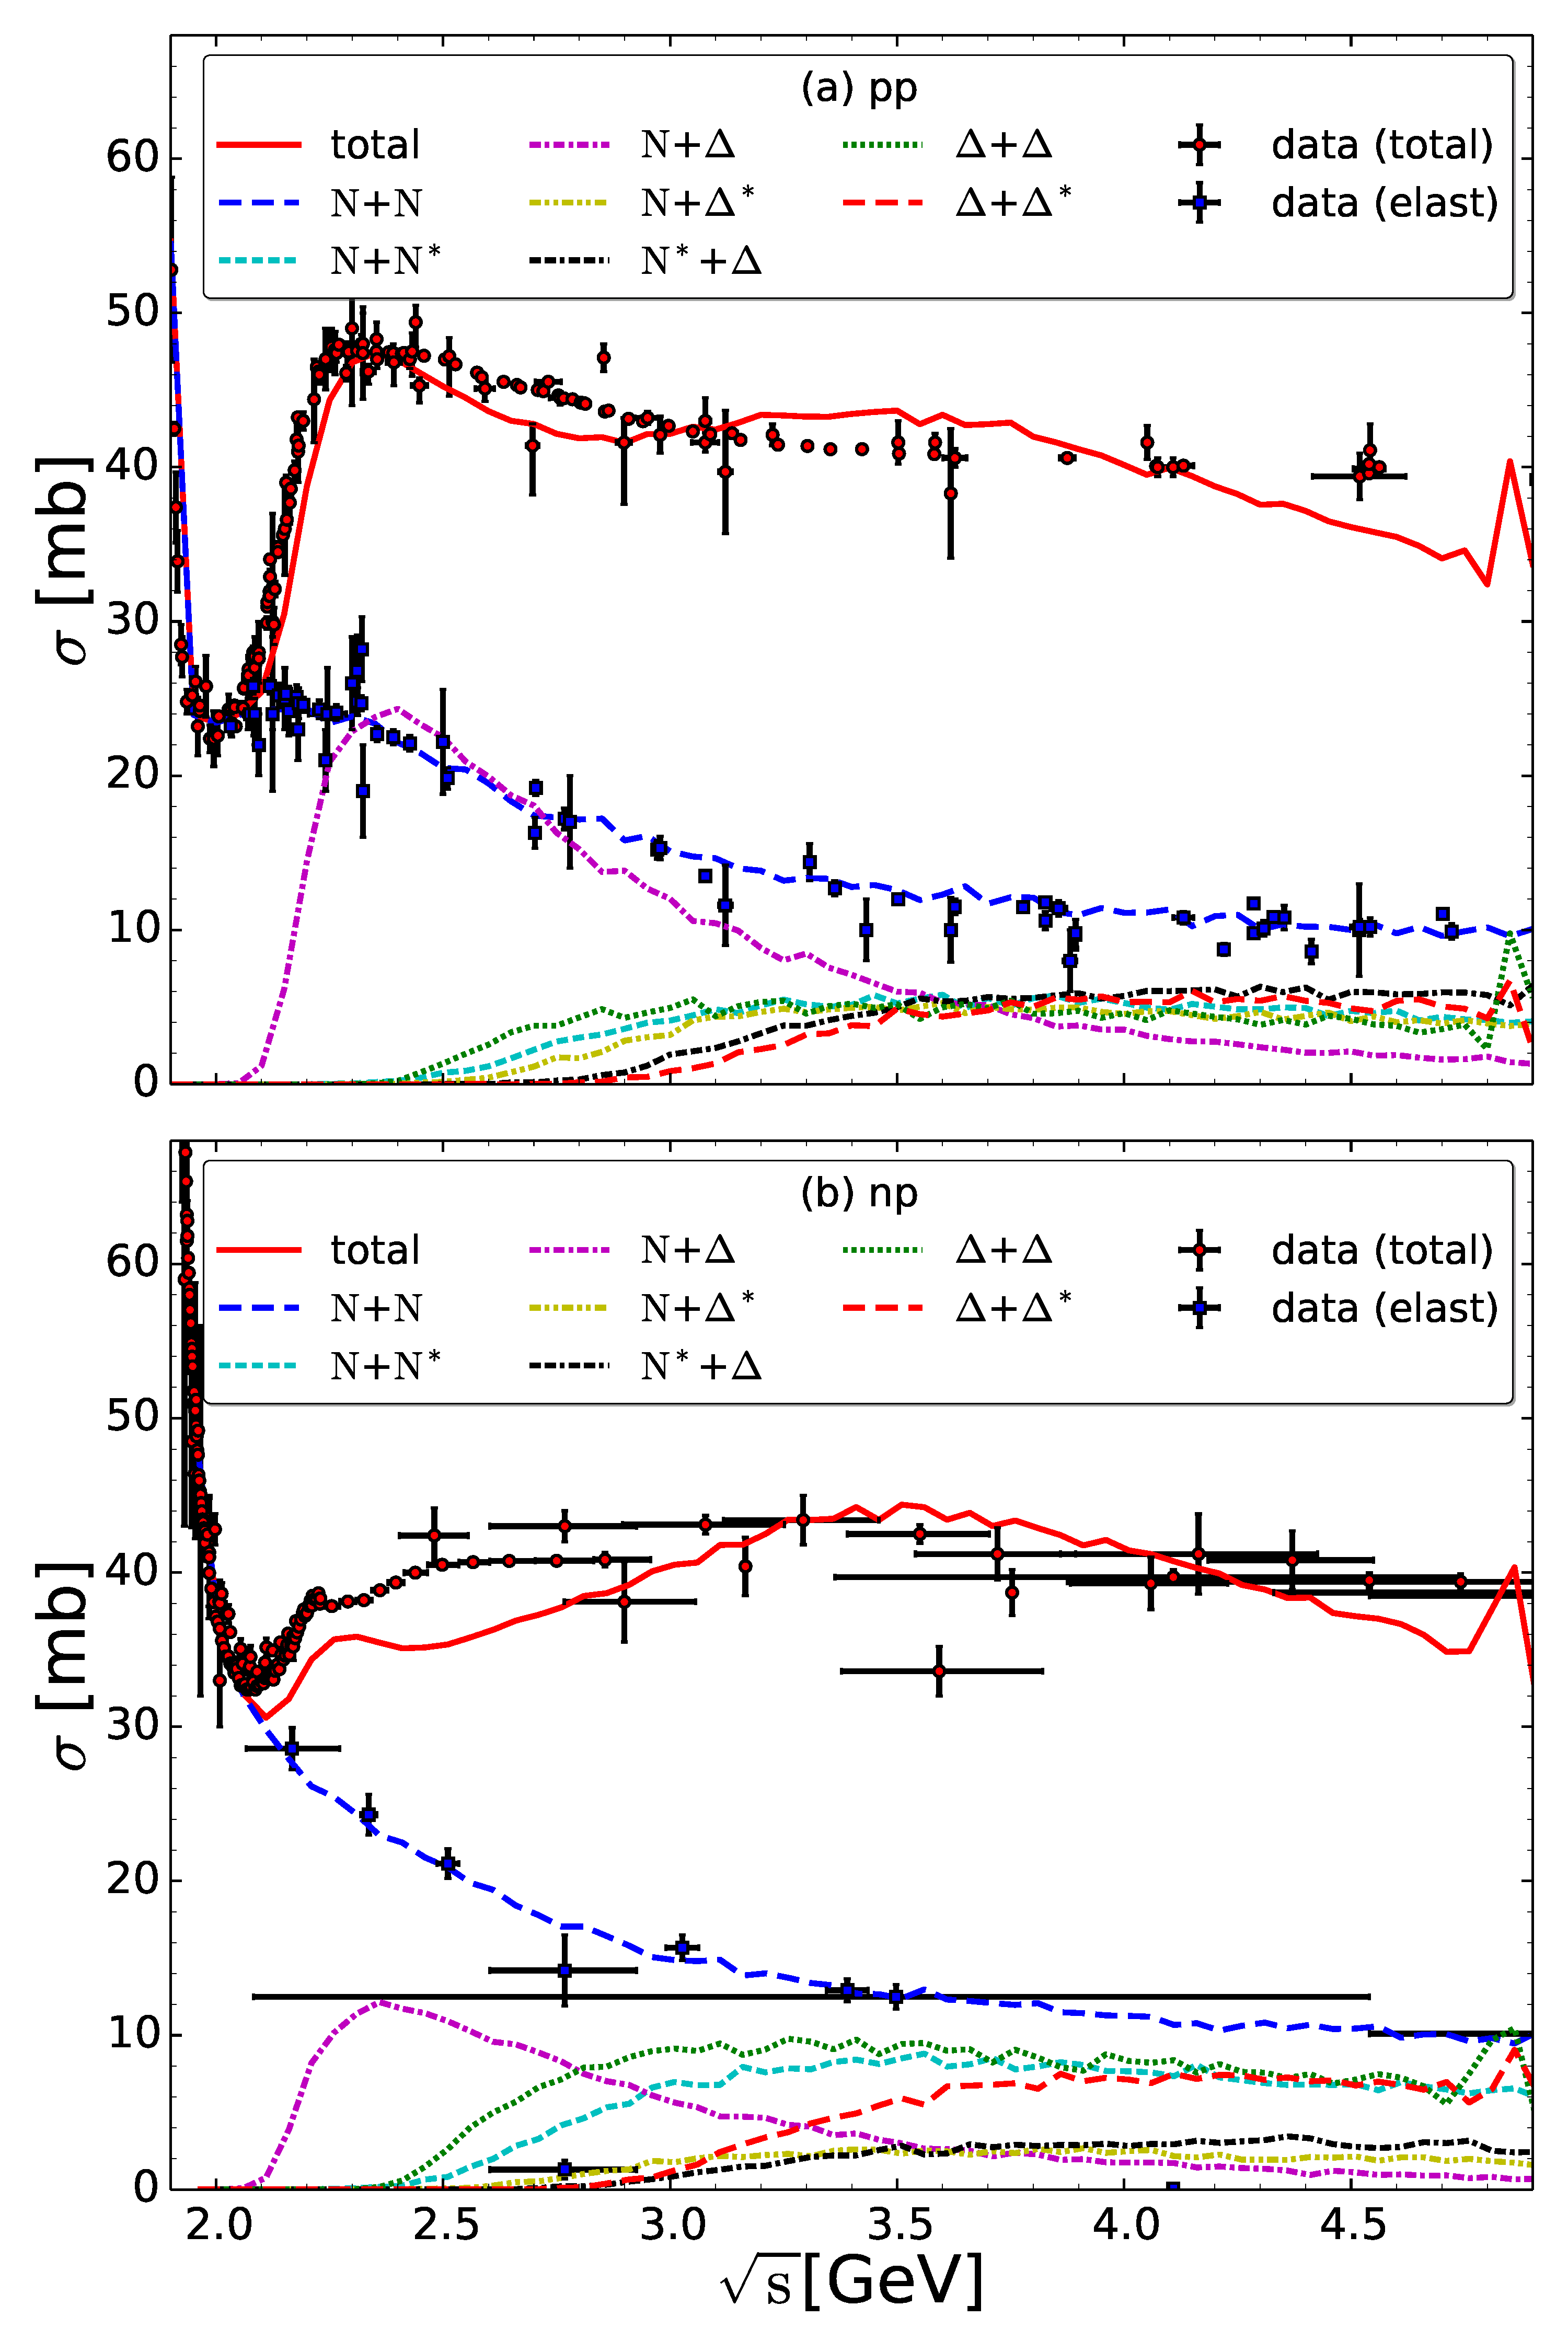
\includegraphics[width=0.49\textwidth]{plots/smash/NN.pdf}\\
  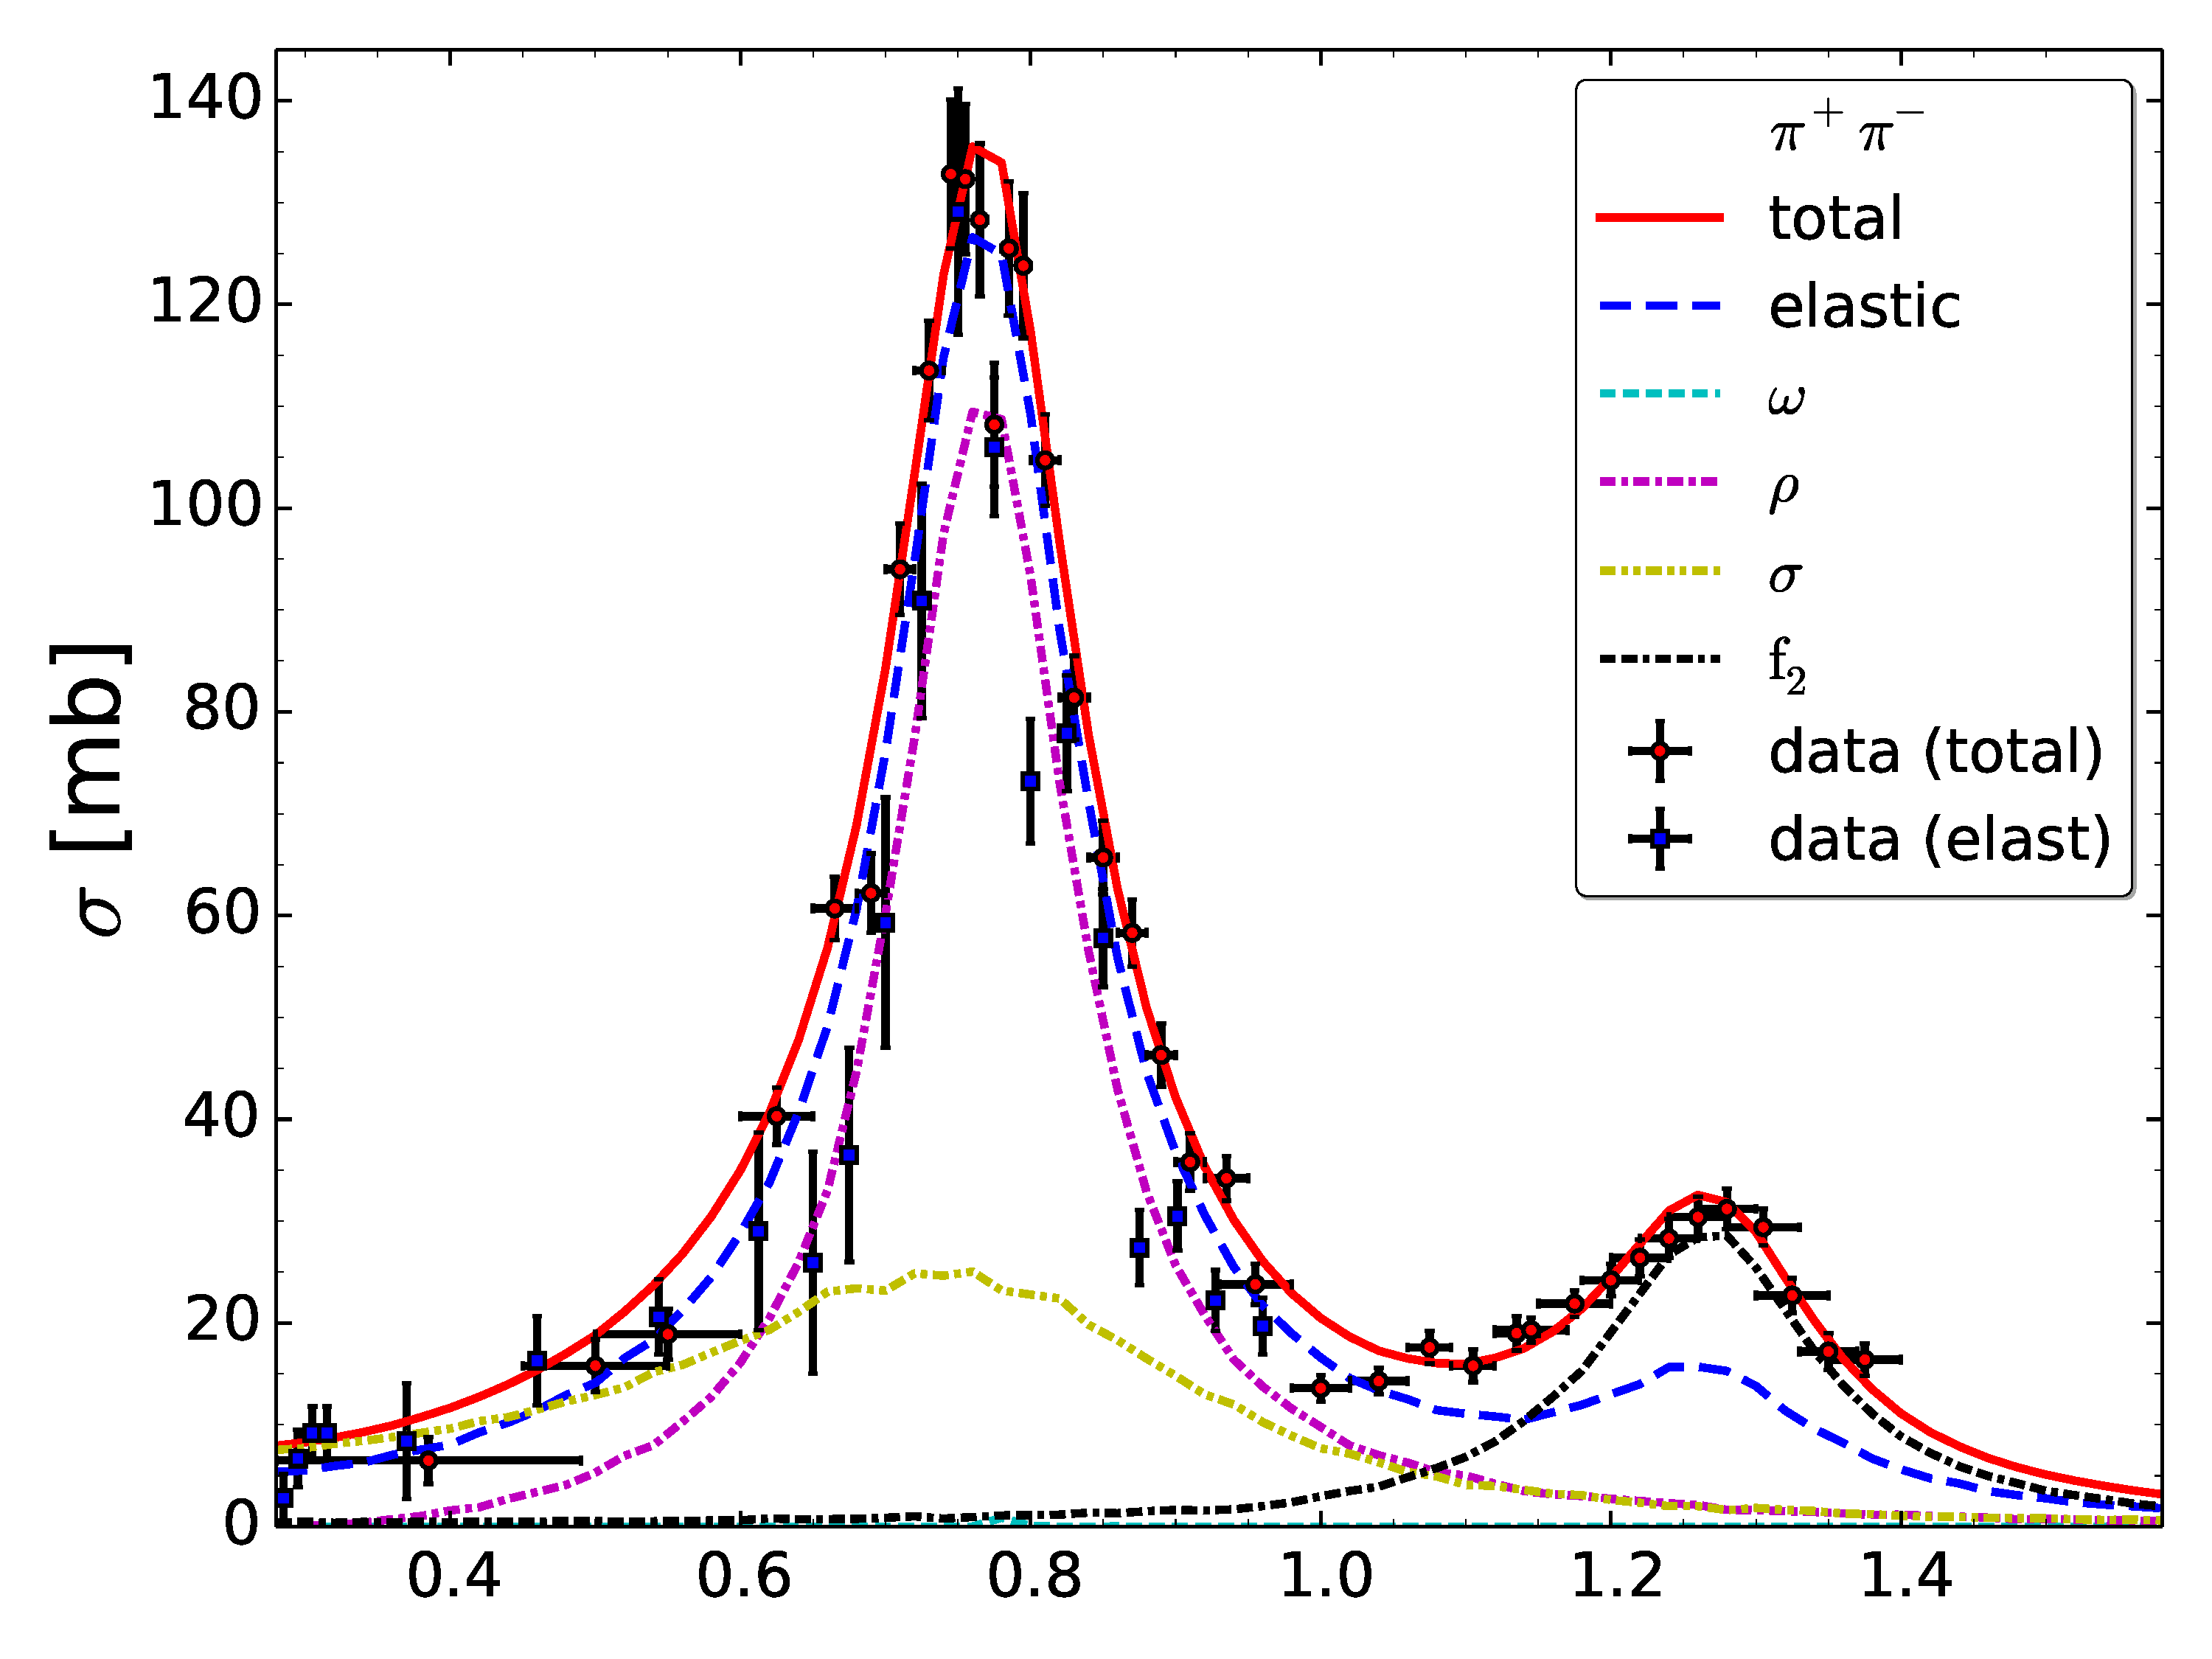
\includegraphics[width=0.5\textwidth]{plots/smash/pipi.pdf}

  \caption{Left upper panel: $\pi^-$-proton (a) and $\pi^+$-proton (b) cross-sections
                             compared to data from \cite{Agashe:2014kda}.
           Right upper panel: Proton-proton (a) and proton-neutron (b) cross-sections
                              compared to data from \cite{Agashe:2014kda}.
           Lower panel: pion-pion cross-section compared to data
                        from \cite{Protopopescu:1973sh,Alekseeva:1982uy}.}
  \label{fig:xs}
\end{figure}

\subsubsection{Angular distributions}
\label{sec:angular}

Anisotropic angular distributions are currently implemented only for
$NN\rightarrow NN$, $NN\rightarrow N\Delta$ and $NN\rightarrow NR$ (with
$R=N^*,\Delta^*$). For elastic nucleon-nucleon collisions the
prescription by Cugnon et al.~\cite{Cugnon:1996kh} is followed, using an exponential ansatz
$d\sigma/dt\propto e^{-bt}$, with an energy-dependent parameter b which is fit
to data. In the second case SMASH also follows Cugnon et al.~\cite{Cugnon:1996kh},
using the same ansatz as for elastic NN collisions. For the last case of
$NN\rightarrow NR$ the ansatz $d\sigma/dt\propto t^{-a}$ is used, with
parameters $a$ which fitted to HADES data \cite{Agakishiev:2014wqa}.
Note that in the present implementation of SMASH all resonances decay
isotropically.

\begin{figure}
  \centering
  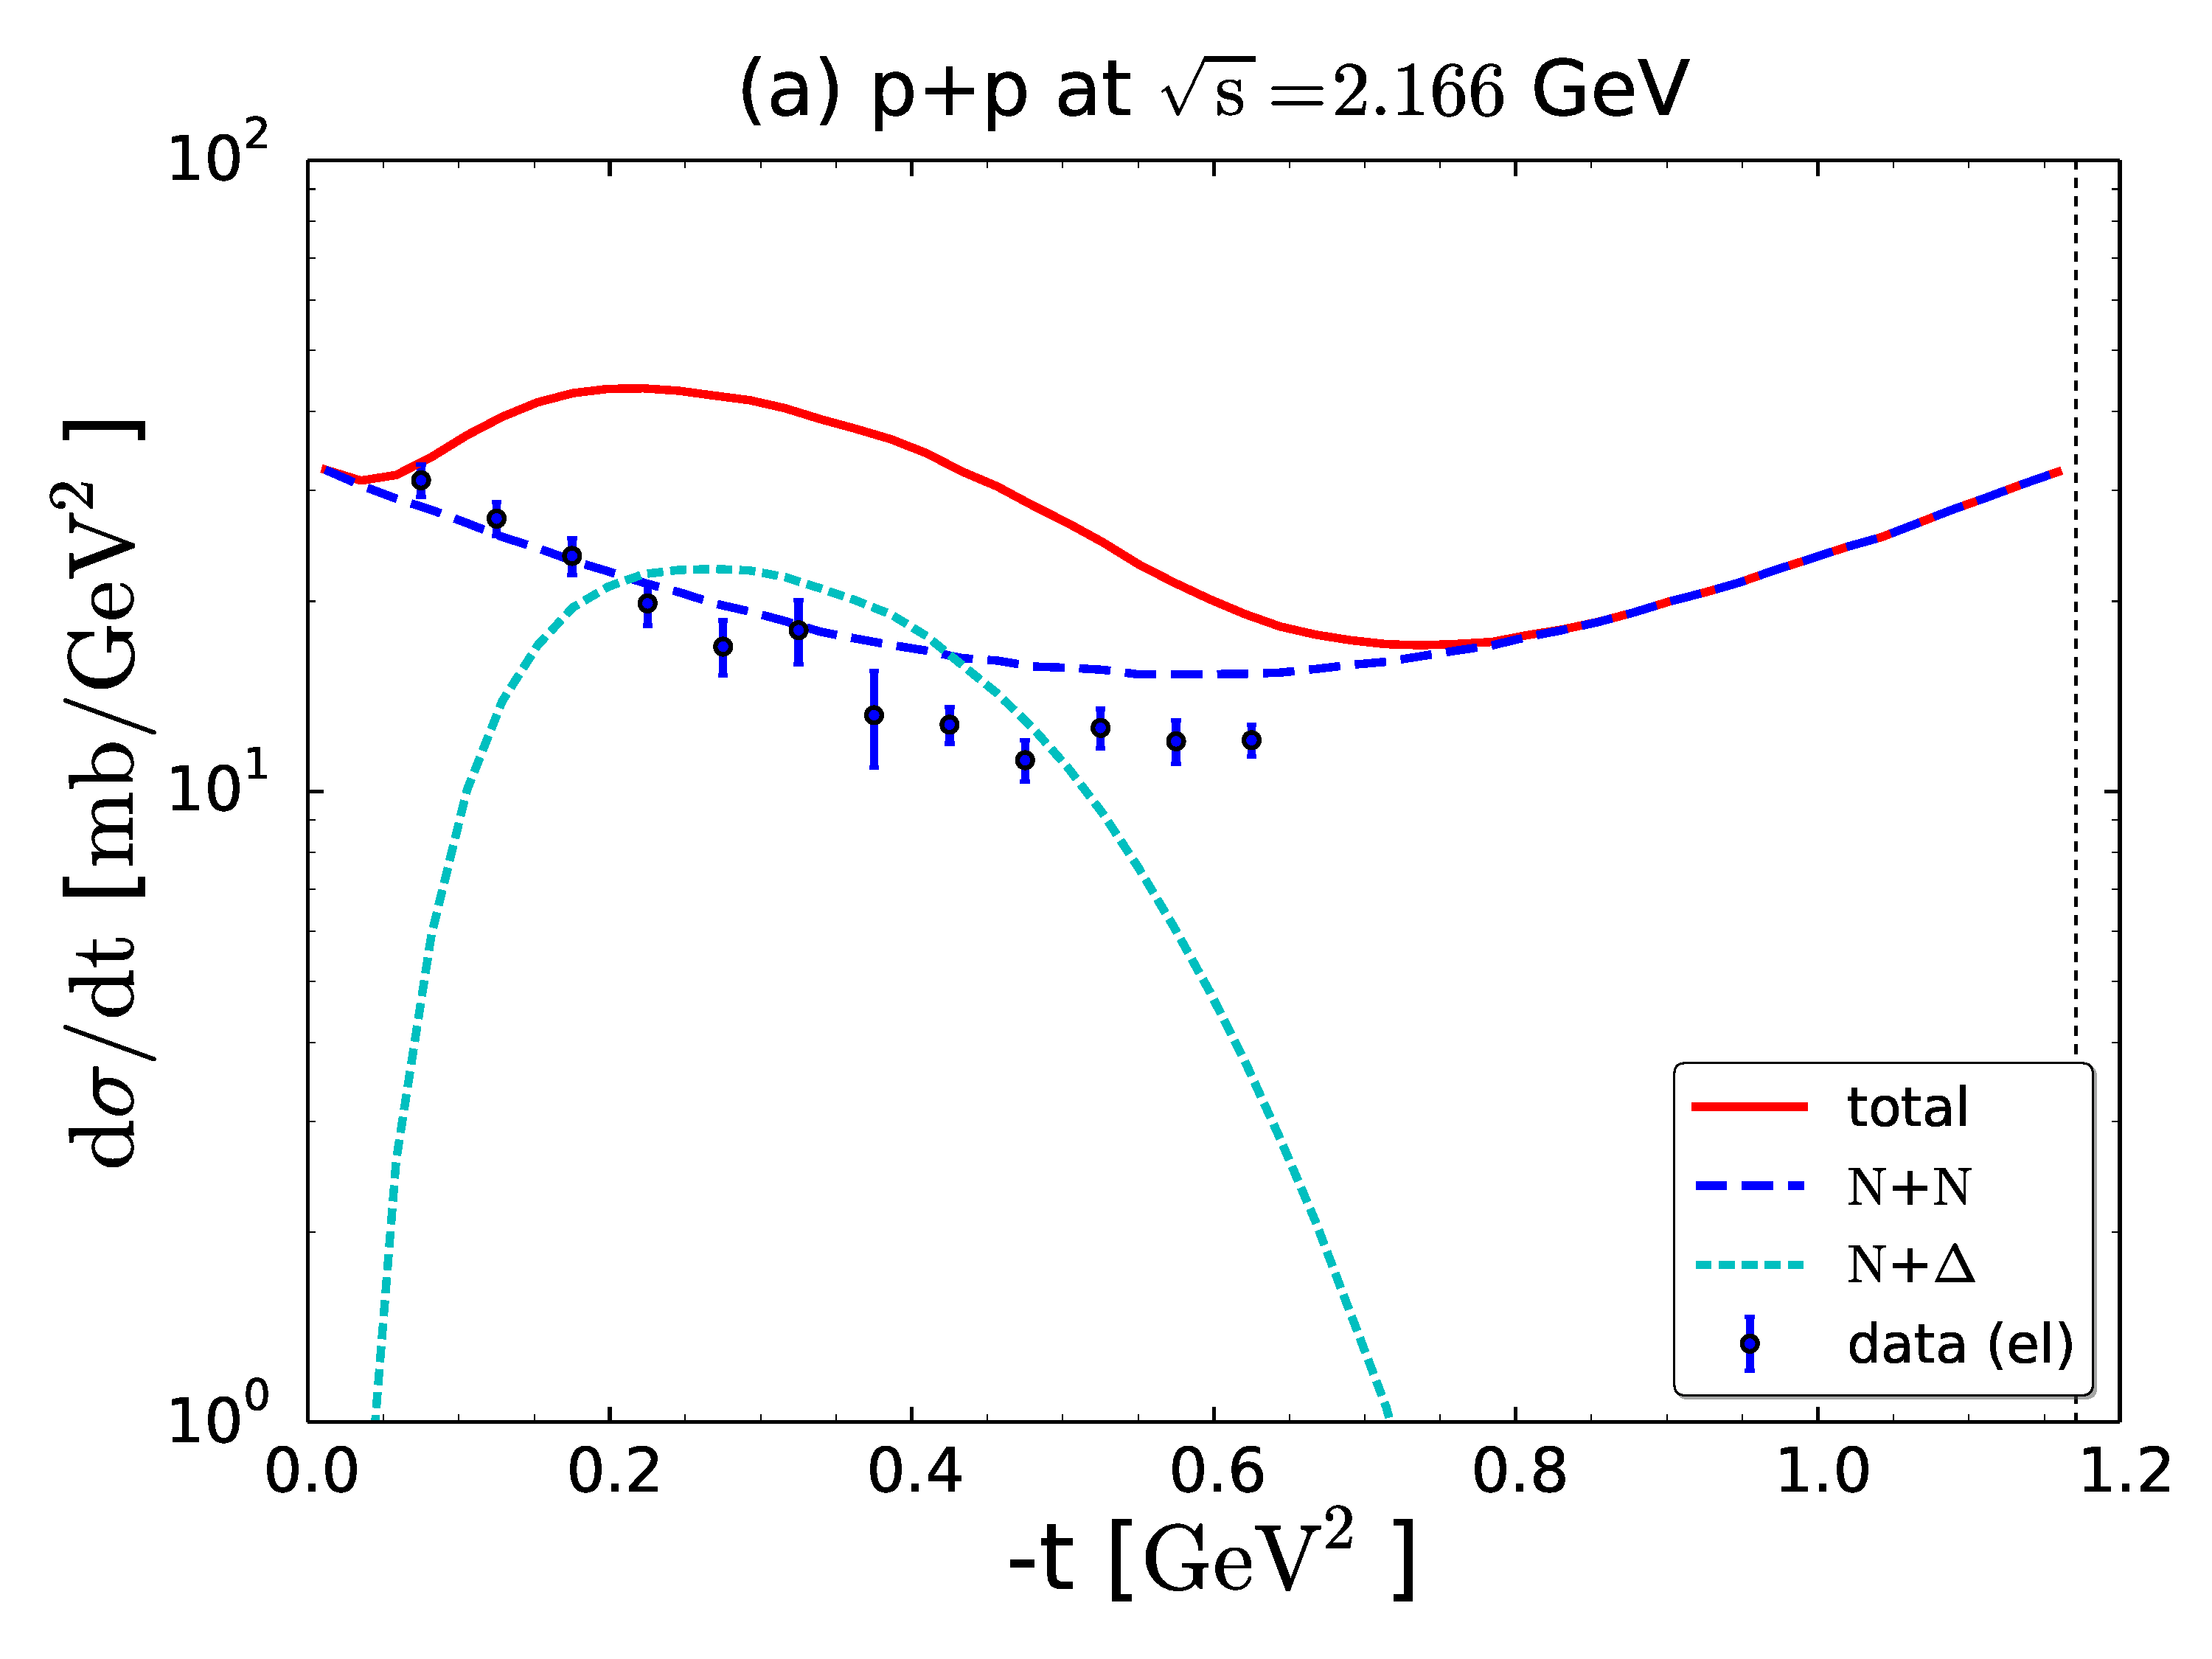
\includegraphics[width=0.48\textwidth]{plots/smash/angular/pp_1.25/t.pdf}
  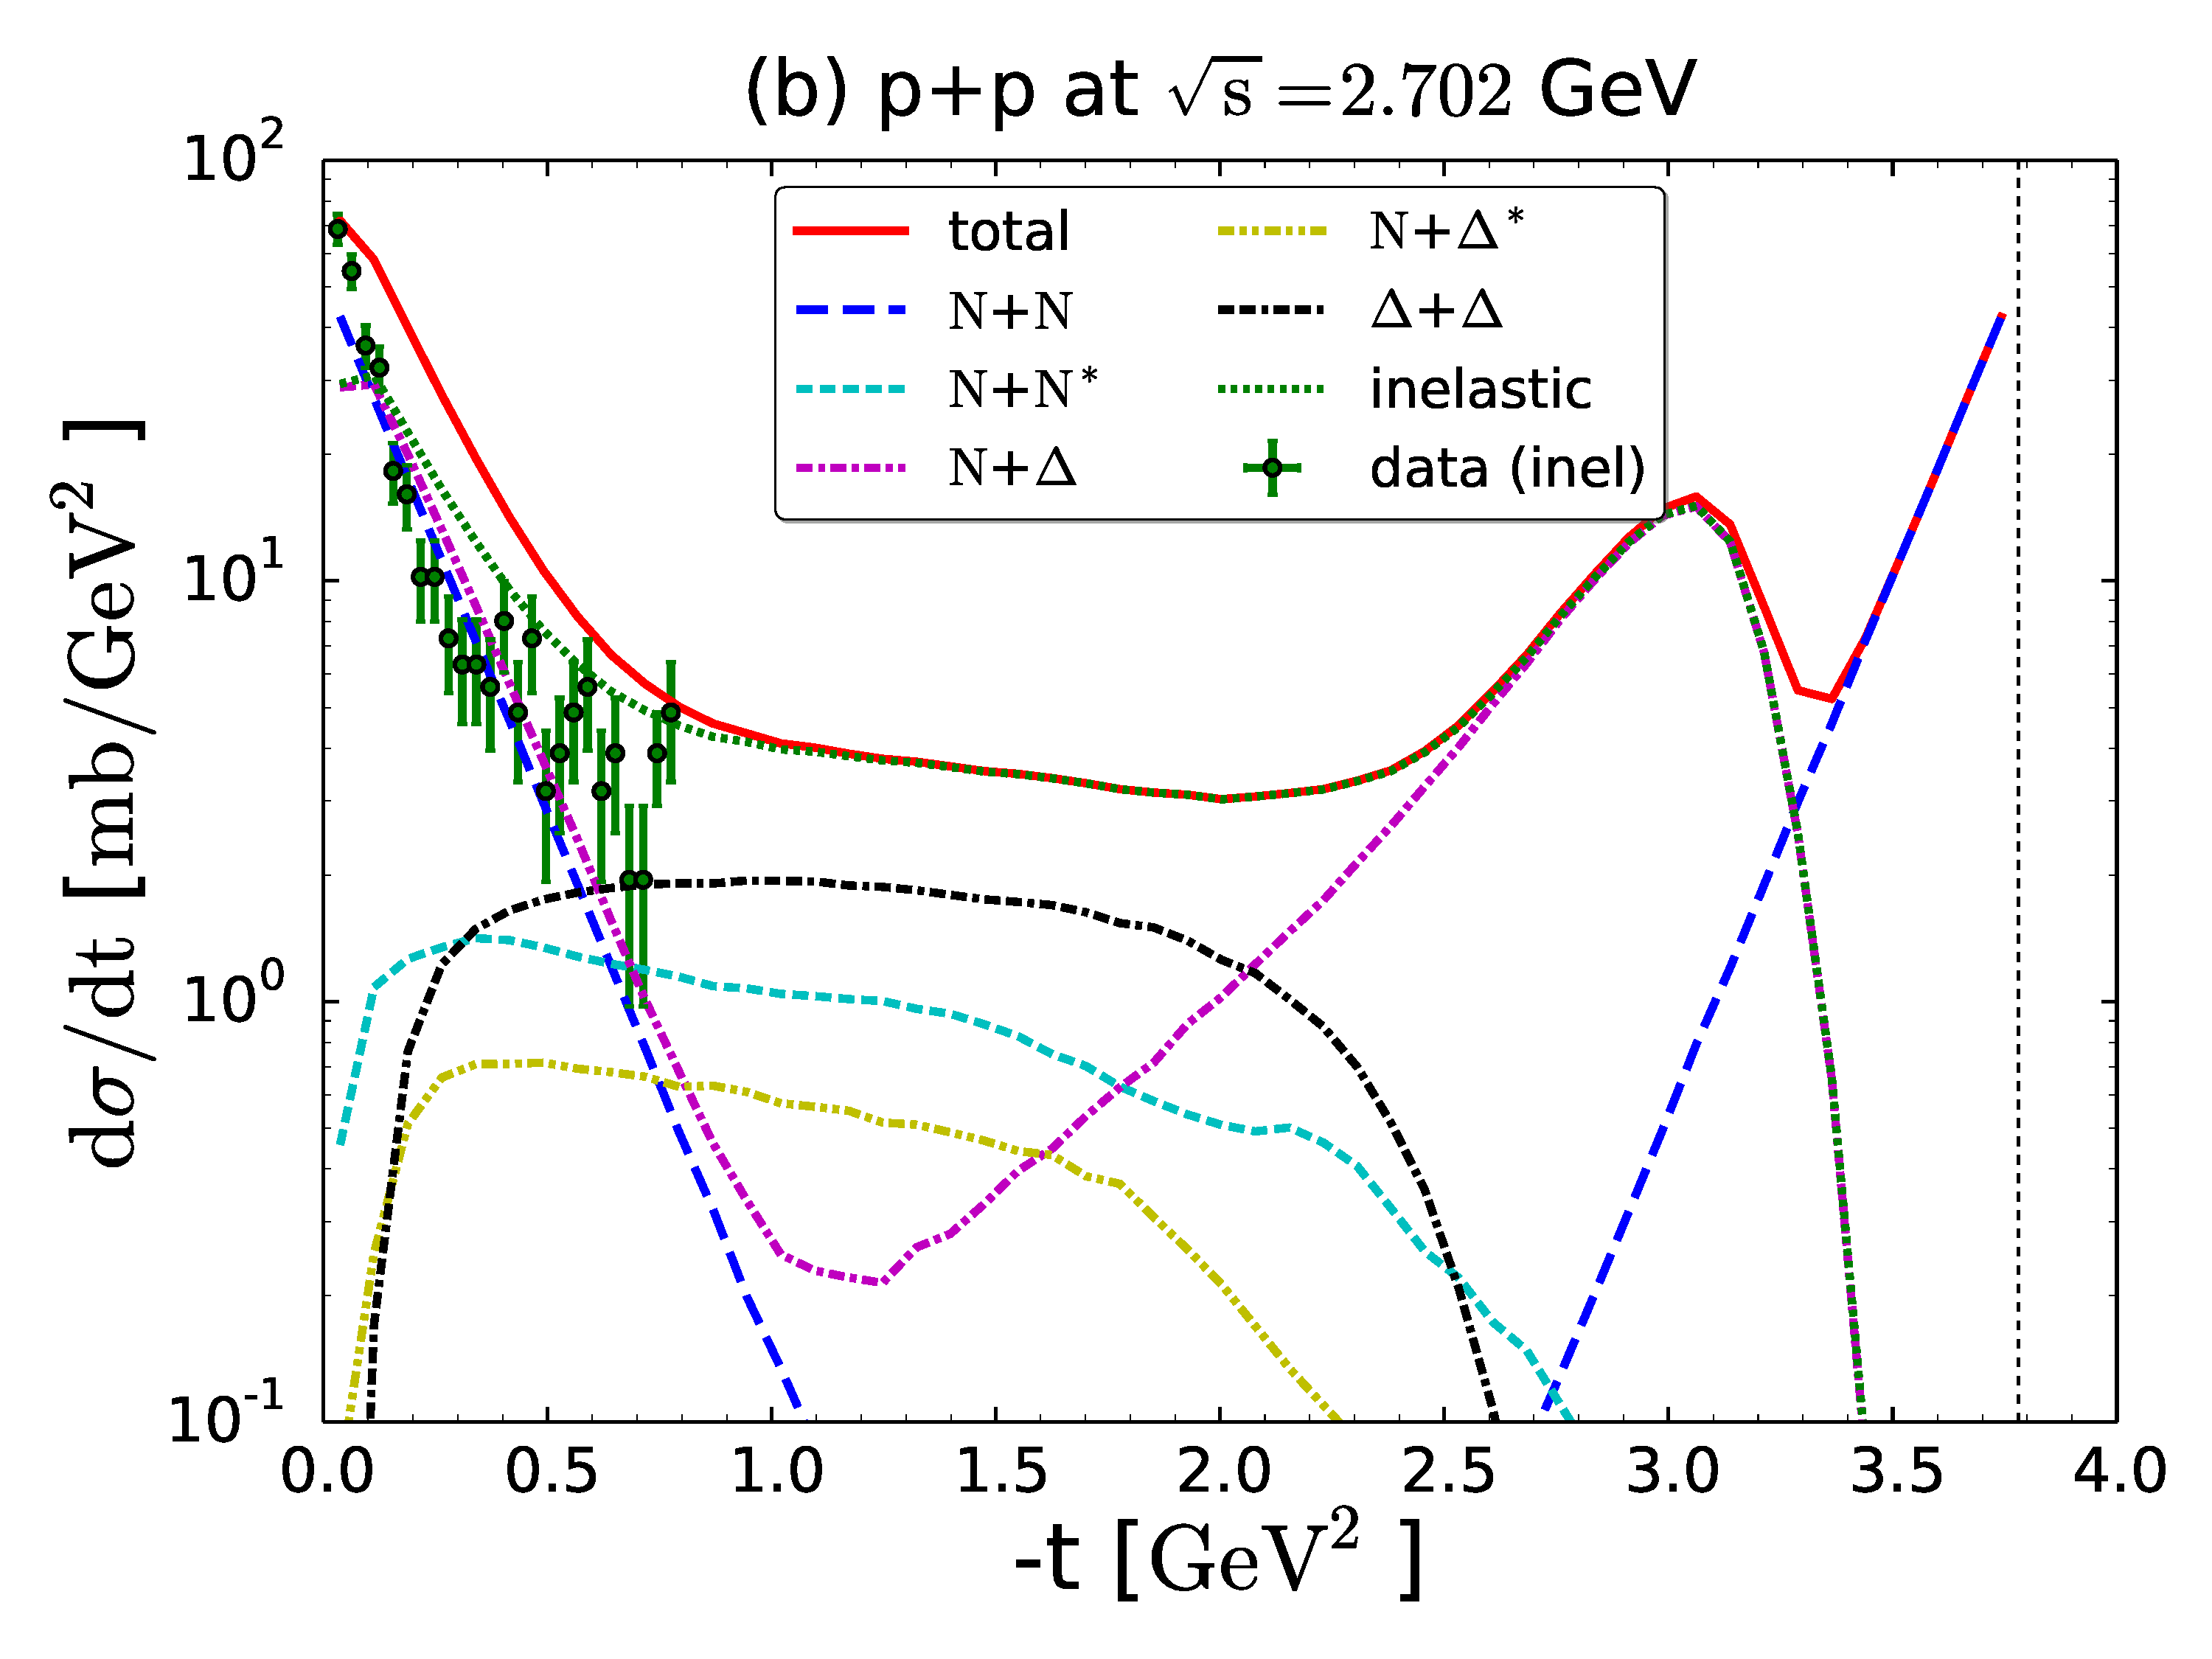
\includegraphics[width=0.48\textwidth]{plots/smash/angular/pp_2.8/t.pdf}
  \caption{Angular distributions for elastic and inelastic pp collisions
           at two different energies, compared to data from \cite{Bacon:1967zz,Ryan}.}
  \label{fig:angular}
\end{figure}

In Fig. \ref{fig:angular} two examples of angular distributions $d\sigma/dt$ in
pp collisions are shown, $t$ being the Mandelstam variable. The upper plot
demonstrates a collision at a relatively low energy, where essentially only the
elastic and single-$\Delta$-production channels are open. The angular
distribution of the elastic channel is of course symmetric in the allowed
$t$-range and matches the data points rather well, even though the slope at
this particular energy appears to be slightly too flat.  The distribution for
single-$\Delta$ production is not symmetric and restricted to a smaller range
in $t$, due to the larger mass of the $\Delta$ in the final state.
Unfortunately there is no inelastic data to compare to at this energy.

The lower plot in Fig. \ref{fig:angular} shows a pp collision at a somewhat
higher energy, where additional resonance production channels are open. In
principle the distributions for all these channels are forward/backward-peaked
(either exponential or power-law shaped). This forward/backward peaking is
clearly visible for the $NN$ and $N\Delta$ final states at least, while those
final states with heavier resonances exhibit a more plateau-like structure, due
to the limited phase space and the mass distributions of the resonances. Here
the sum of all inelastic channels is compared to data and indeed shows a
reasonable agreement, again with a slight tendency of being too flat.



\subsection{Decays}

In section \ref{sec:spectral_function} the time-dependent propagator
(Eq. \ref{eq:t_dep_propagator}) was considered to derive the spectral
function of hadrons. This propagator can be integrated for $t > 0$
by contour integration resulting in

\begin{equation}
  \mathcal{G}(p,t) = \frac{i}{2\sqrt{\vec{p}^2 + M_0^2 - i M_0 \Gamma}}
                     \expOf{-i t \sqrt{\vec{p}^2 + M_0^2 - i M_0 \Gamma}} \,.
\end{equation}

Assuming that $\Gamma \ll M_0$, one rewrites $\sqrt{\vec{p}^2 + M_0^2 - i M_0
\Gamma} = E - \frac{i M_0 \Gamma}{2 E}$ and obtains

\begin{equation}
  \mathcal{G}(p,t) = \frac{i}{2 E} e^{-i E t} \expOf{\frac{- M_0 \Gamma}{2 E} t}
\end{equation}

Therefore the probability to find the resonance decays exponentially. The lifetime
$\tau$ is determined according to

\begin{equation}
  \tau = \frac{E}{M_0} \frac{1}{\Gamma(m)} \,.
\end{equation}

The factor $\frac{E}{M_0}$ corresponds to the time dilation. In SMASH the lifetime
of the particle is sampled from the exponential distribution:

\begin{equation}
  P(\text{decay in the interval}(t, t+dt]) = \frac{dt}{\tau} e^{-t/\tau} \,.
\end{equation}

The width $\Gamma(m)$ is computed according to section \ref{sec:width}.
SMASH has only 2-body decays to maintain detailed balance. All the resonance
decays are assumed to be isotropic in the resonance rest frame.

\subsection{Detailed balance} \label{sec:det_bal}

Detailed balance is an important principle that allows to express properties
of the reverse reaction, if the properties of the forward reaction are known.
Several equivalent statements are referred to as the principle of detailed balance:

\begin{itemize}
  \item In thermal equilibrium the rate of forward reactions is equal
        to the rate of reverse reactions for every reaction in any region
        of phase space \cite{Lifsh10}.
  \item Matrix elements of the forward reaction are equal to the matrix
        elements of the reverse  reaction.
  \item A particular relation holds between the differential cross-sections
        of forward and reverse reaction or between the width of $1 \to 2$
        and the cross-section of the reverse $2 \to 1$ reaction.
\end{itemize}

\subsubsection{Time reversal and detailed balance principle} \label{sec:smatrix}

The equality of the matrix elements of the forward and reverse reaction can be
derived from the time-reversal invariance of the $S$-matrix. Here for
completeness the derivation given in different paragraphs of textbook \cite{Lifsh4} is
put together. This reproduction is useful to

\begin{itemize}
  \item introduce the concept of matrix elements and cross-sections, which are used
        throughout the text
  \item outline the connection between the time-reversal invariance and detailed
        balance
  \item set the stage for the derivation of the detailed balance relations for the
        reactions involving unstable particles
\end{itemize}

Let $\ket{i}$ be an initial state and $\ket{f}$ a final state wavefunctions of
the scattering. The initial state  can be written as

\begin{equation}
  \ket{i} = \sum_{f} \ket{f} \bra{i} S \ket{f} \,,
\end{equation}

where the sum is taken over all possible final states. Here the operator $S$ is
connected to the Lagrangian via the formal solution of the equations of motion

\begin{equation}
  S = T \, exp \left(\int \mathcal{L}_{int} d^4x \right) \,,
\end{equation}

where $T \, exp$ denotes time-ordered exponential, $\mathcal{L}_{int}$ is
interaction part of Lagrangian. This expression can be further expanded into
formal series, where each term corresponds to Feynmann diagrams of a particular
order. Matrix $S_{if} = \bra{i} S \ket{f}$ is called scattering matrix or
S-matrix. Quantities $|S_{if}|^2$ are probabilities to go from state
$|i\rangle$ to state $|f\rangle$. Taking into account that for the absence of
scattering $S_{if} = \delta_{if}$ and energy-momentum conservation, it is
convenient to rewrite

\begin{equation}
  S_{if} \equiv \Braket{i|f}  = \delta_{if} + i(2\pi)^4 \delta^{(4)}(P_i-P_f) T_{if} \,,
\end{equation}

where factor $i (2\pi)^4$ is there just for further convenience, and $P_i$ and $P_f$ are the 4-momenta of the initial and final states. Computing
$|S_{if}|^2$ one obtains the delta-function squared, a common artifact in field
theory. One of the delta-functions can be rewritten as

\begin{equation}
  \delta^{(4)}(P_i-P_f) = (2\pi)^{-4} \int e^{i(P_i-P_f)x} d^4x
\end{equation}

Since first of delta functions sets $P_i=P_f$, this one can be interpreted as
$(2\pi)^{-4} Vt$, where integration over $d^4x$ is performed over the finite volume
and time. So, for the non-diagonal elements

\begin{equation} \label{eq:sif_sqr}
|S_{if}|^2 = (2\pi)^4 \delta^{(4)}(P_i-P_f) |T_{if}|^2 Vt
\end{equation}

It turns out that in momentum representation wavefunctions that stand in
$T_{if}$ have structure like $(2 E V)^{-1/2} \left(\hat{a} e^{-ipx}
+\hat{a}^{\dag} e^{ipx}\right)$. Therefore, for reaction $p_1+p_2 \to p_1' +
p_2'$ \footnote{In this chapter capital $P$ denotes 4-momenta, small $p$ denotes 3-momenta.} it is
convenient to introduce

\begin{equation}
  M_{if} = (2 E_1 V)^{-1/2} (2 E_2 V)^{-1/2} (2 E_1' V)^{-1/2} (2 E_2' V)^{-1/2} T_{if}
\end{equation}

Object $M_{if}$ is called the matrix element. For the strong interaction time reversal
is a strict symmetry. This means that the $S$-matrix has the following
 property \cite{Sachs_time_reversal}:

\begin{equation}
   S_{if} \equiv \Braket{i|f} = e^{i(\varphi_i - \varphi_f)} \Braket{f|i} =
   S_{fi} e^{i(\varphi_i - \varphi_f)}
\end{equation}

From this relation it follows that

\begin{equation} \label{eq:detbal_matr_el}
  |M_{if}|^2 = |M_{fi}|^2
\end{equation}

Let us prove that Eq. (\ref{eq:detbal_matr_el}) is enough for the rates
of forward and reverse reactions to be identical in equilibrium. The proof
is presented for $2 \to 2$ reactions, but it can be extended analogously for any other
collisions. The probability to scatter with final momenta $p_1'$ and $p_2'$ per unit
time follows from Eq. (\ref{eq:sif_sqr}):

\begin{equation} \label{eq:scat_prob}
  dw = (2\pi)^4 \delta^{(4)}(P_i-P_f)
       |M_{if}|^2 \frac{1}{4 E_1 E_2 V}
       \frac{d^3p_1'}{2E_1' (2\pi)^3}
       \frac{d^3p_2'}{2E_2' (2\pi)^3}
\end{equation}

Additionally, there is a  factor $1/2$, if the particles in the final state are
identical. It follows that the numbers of the forward and reverse
reactions (denoting $d^4 \Omega_p = \frac{d^3p_1}{2E_1} \frac{d^3p_2}{2E_2}
\frac{d^3p'_1}{2E'_1} \frac{d^3p'_2}{2E'_2}$) are

\begin{align}
  dN_{\rightarrow} &=& (2\pi)^{-2} \delta^{(4)}(P_i-P_f) |M_{if}|^2 d^4 \Omega_p \, \mathit{f}(p_1) \mathit{f}(p_2) \parenths{1 \pm \mathit{f}(p'_1)} \parenths{1 \pm \mathit{f}(p'_2)} \\
  dN_{\leftarrow}  &=& (2\pi)^{-2} \delta^{(4)}(P_i-P_f) |M_{if}|^2 d^4 \Omega_p \, \mathit{f}(p'_1) \mathit{f}(p'_2) \parenths{1 \pm \mathit{f}(p_1)} \parenths{1 \pm \mathit{f}(p_2)}
\end{align}

In thermal equilibrium the parts of $dN_{\rightarrow}$ and
$dN_{\leftarrow}$ related to the distributions are identical, therefore
in thermal equilibrium

\begin{equation} \label{eq:det_bal_reactions}
  dN_{\rightarrow} = dN_{\leftarrow}
\end{equation}

Finally, it is important to note that although this relation was derived from
time-reversal invariance, it can also hold if the invariance is broken
\cite{Sachs_time_reversal}. Further the detailed balance relation represented
by Eq. (\ref{eq:detbal_matr_el}) is linked to the cross-sections.


\subsubsection{Detailed balance relations for $ 2\to 2$ reactions} \label{sec:detbal_2to2}

The cross-section $\sigma$ is defined in the rest frame of the target
via an expression for the number of interactions

\begin{equation}
  dN_{inter} = \sigma v_{rel} n_1 n_2 dV dt
\end{equation}

The factor after the cross-section is often called luminosity. This expression can
be written for any frame in the Lorentz-invariant form \cite{Lifsh2}:

\begin{equation}
  dN_{inter} = \sigma \sqrt{(\vec{v_1}-\vec{v_2})^2 + [\vec{v_1}\times \vec{v_2}]^2}
  n_1 n_2 dV dt = \sigma \frac{\sqrt{(P_1 \cdot P_2)^2 - m_1^2 m_2^2}}{E_1 E_2}
  n_1 n_2 dV dt
\end{equation}

The probability to scatter from Eq. (\ref{eq:scat_prob}) is connected
to the cross-section via

\begin{equation}
  dw = V^{-1} \sigma  \sqrt{(\vec{v_1}-\vec{v_2})^2 + [\vec{v_1}\times \vec{v_2}]^2} \,,
\end{equation}

where $n_1 = n_2  = V^{-1}$ was assumed. Let us denote
$I = \sqrt{(P_1 \cdot P_2)^2 - m_1^2 m_2^2}$. Then

\begin{equation}
  d\sigma = (2\pi)^{-2} \delta^{(4)}(P_i-P_f) |M_{if}|^2 \frac{1}{4 I}
  \frac{d^3p_1'}{2E_1'} \frac{d^3p_2'}{2E_2'} \frac{1}{1+\delta_{1'2'}}
\end{equation}

The last factor $\frac{1}{1+\delta_{1'2'}}$ accounts for identical particles in
the final state. The total cross-section is the integral of this expression. For the
case where the outgoing particles are resonances the following trick from
\cite{Wolf:1992qja} is applied

\begin{equation}
  \frac{d^3p}{2E} = \delta(P^2 - m^2) d^4p = \frac{d^3p}{2E} \delta(M^2 - m^2) dM^2 \,,
\end{equation}

where a transformation from variables $E,\vec{p}$ to $M^2 = E^2 - \vec{p}^2,
\vec{p}$ was performed. For resonances in the final state one substitutes
the spectral function of the resonance $\mathcal{A}(M^2)$ instead of $\delta$-function.
Therefore,

\begin{equation} \label{eq:sigma22}
  d\sigma = (2\pi)^{-2} \delta^{(4)}(P_i-P_f) |M_{if}|^2 \frac{1}{4 I}
            \frac{d^3p_1'}{2E_1'} \frac{d^3p_2'}{2E_2'} \frac{1}{1+\delta_{1'2'}}
            \mathcal{A}_1(M_1'^2) \mathcal{A}_2(M_2'^2) dM_1'^2 dM_2'^2
\end{equation}

The whole expression is Lorentz invariant and the integration over
the momenta is easy to perform in the center of mass frame.

\begin{eqnarray}
  \delta^{(4)}(P_i-P_f) \frac{d^3p_1'}{2E_1'} \frac{d^3p_2'}{2E_2'} \to
  \delta(E_1+E_2 - E_1'- E_2') \frac{d^3p_1'}{4E_1'E_2'} \\
  d^3p_1' = p_{cm}^2 dp_{cm} d\Omega \\
  d(E_1'+ E_2') = d \parenths{\sqrt{p_{cm}^2 +M_1^2} +\sqrt{p_{cm}^2 +M_2^2}} =
  \parenths{\frac{1}{E_1'} + \frac{1}{E_2'}} p_{cm} dp_{cm}
\end{eqnarray}

Here $p_{cm}$ is the momentum of the reaction products in the center of mass frame,
which was introduced in Eq. (\ref{eq:p_cm}). After the change of variables to
$E_1'+ E_2'$ and integration over the remaining delta-function, taking into
account that in the CM-frame $(E_1+E_2)^2 = s$ and $I = p_{cm} (E_1+E_2)$,

\begin{equation}
  d\sigma/d\Omega = \frac{1}{64\pi^2 s} |M_{if}|^2 \frac{p_{cm}(s, M_1',M_2')}{p_{cm}(s, m_1,m_2)}
  \frac{1}{1+\delta_{1'2'}} \mathcal{A}_1(M_1'^2) \mathcal{A}_2(M_2'^2) dM_1'^2 dM_2'^2
\end{equation}

Finally, in SMASH spin is not an explicit degree of freedom and one has to average
matrix element over spins of the produced particles:

\begin{equation}
  d\sigma/d\Omega =
  \frac{1}{64\pi^2 s} \frac{(2S_1'+1)(2S_2'+1)}{1+\delta_{1'2'}}|M_{if}|^2
  \frac{p_{cm}(s, M_1',M_2')}{p_{cm}(s, m_1,m_2)}
  \mathcal{A}_1(M_1'^2) \mathcal{A}_2(M_2'^2)  dM_1'^2 dM_2'^2
\end{equation}

For numerical simulations it is useful to obtain expressions connecting the cross-
section of the forward reaction to the one of the reverse reaction. It is assumed that
in the forward reaction two incoming particles are stable with pole masses $m_1$ and
$m_2$ and the outgoing particles are possibly unstable and their off-shell
masses are not yet known, they will only be sampled after the cross-section is
computed and the reaction takes place.  In this way it is easy to understand
why the forward reaction cross-section is averaged over the spectral functions
of products.

\begin{equation} \label{eq:cs_forward22}
  d\sigma_{12 \to 1'2'}/d\Omega =
  \frac{1}{64\pi^2 s} \frac{(2S_1'+1)(2S_2'+1)}{1+\delta_{1'2'}}|M_{if}(s)|^2 \times \nonumber \\
  \frac{  \int p_{cm}(s, M_1',M_2') \mathcal{A}_1(M_1'^2) \mathcal{A}_2(M_2'^2)  dM_1'^2 dM_2'^2 }
  {p_{cm}(s, m_1,m_2)}
\end{equation}

In the reverse reaction incoming products already have particular off-shell
masses $M_1$ and $M_2$ and they will form stable particles with masses $m_1$ and
$m_2$. Then for the reverse reaction

\begin{equation} \label{eq:cs_reverse22}
  d\sigma_{1'2' \to 12}/d\Omega =
  \frac{1}{64\pi^2 s} \frac{(2S_1+1)(2S_2+1)}{1+\delta_{12}}|M_{fi}(s)|^2
  \frac{p_{cm}(s, m_1,m_2)} {p_{cm}(s, M_1,M_2)}
\end{equation}

The matrix elements in Eqs. (\ref{eq:cs_forward22} - \ref{eq:cs_reverse22}) are equal
as discussed in section \ref{sec:smatrix}. Dividing the Eq. (\ref{eq:cs_forward22})
over the Eq. (\ref{eq:cs_reverse22}) one obtains the detailed balance relation
for cross-sections

\begin{align}
  \frac{d\sigma_{12\to 1'2'}/d\Omega}{d\sigma_{1'2'\to 12}/d\Omega} =
  \frac{(2S_1'+1)(2S_2'+1)}{(2S_1+1)(2S_2+1)} \frac{1+\delta_{12}}{1+\delta_{1'2'}} \times \nonumber \\
  \frac{p_{cm}(s, M_1,M_2)\int p_{cm}(s, M_1',M_2')
  \mathcal{A}_1(M_1'^2) \mathcal{A}_2(M_2'^2) dM_1'^2 dM_2'^2 }{p^2_{cm}(s, m_1,m_2)}
\end{align}


\subsubsection{Detailed balance relations for $ 2\to 1$ reactions} \label{sec:detbal_2to1}

Similarly to equation (\ref{eq:sigma22}) for $2 \to 2$ reactions one can
express the cross-section for $ 2\to 1$ reactions $ab \to R$ with masses
$m_1$, $m_2$ and $M_R$:

\begin{equation} \label{eq:sigma21}
  d\sigma = (2\pi)^{-2} \delta^{(4)}(P_i-P_f) |M_{if}|^2 \frac{1}{4 I}
            \frac{d^3p_R}{2E_R} \mathcal{A}_R(M_R^2) dM_R^2
\end{equation}

Performing the same transformations as for the $2 \to 2$ case and taking into
account that $M_R^2 = s$ one arrives at

\begin{equation} \label{eq:cs_2to1}
  \sigma_{ab\to R} = \frac{\pi}{2} |M_{if}|^2 \frac{1}{\sqrt{s} p_{cm}(\sqrt{s}, m_1, m_2)} \mathcal{A}_R(s)
\end{equation}

For the reverse decay $R \to ab$ with possibly unstable products the
equation (\ref{eq:scat_prob}) for the probability to decay per unit time is
rewritten in the same way as for $2 \to 2$ reactions resulting in

\begin{equation}
  dw = \frac{d\Omega}{(2\pi)^2} |M_{fi}|^2 \frac{ \int p_{cm}(\sqrt{s}, m'_1, m'_2) \mathcal{A}_1(m_1'^2) \mathcal{A}_2(m_2'^2) dm_1'^2 dm_2'^2 }{8 s}
       \frac{1}{1+\delta_{ab}}
\end{equation}

Integrating over $d\Omega$ and recalling that the probability to decay per unit
time is the resonance width $\Gamma$ one finds

\begin{equation} \label{eq:width_1to2}
  \Gamma_{R \to ab} = \frac{|M_{fi}|^2}{8\pi s} \int p_{cm}(\sqrt{s}, m'_1, m'_2) \mathcal{A}_1(m_1'^2) \mathcal{A}_2(m_2'^2) dm_1'^2 dm_2'^2
           \frac{1}{1+\delta_{ab}}
\end{equation}

Note that from this equation follows the expression for the off-shell width,
Eq. (\ref{eq:off_shell_width}), only without the Blatt-Weisskopf factor and the
form factor.  The latter originate from the matrix element, which here is
assumed to depend only on $s$. Averaging matrix elements over spin and
taking the ratio of Eq. (\ref{eq:cs_2to1}) to Eq. (\ref{eq:width_1to2}) one
obtains the detailed balance relation

\begin{equation}
  \sigma_{ab \to R} =  \Gamma_{R \to ab}
                      \frac{2 S_R + 1}{(2 S_1 + 1)(2 S_2 + 1)} \parenths{1+\delta_{ab}}
                      \frac{4 \pi^2 }{p_{cm}(\sqrt{s}, m_1, m_2) \rho(\sqrt{s})}
                      \mathcal{A}_R(s) \\
  \rho(\sqrt{s}) = \int \frac{p_{cm}(\sqrt{s}, m'_1, m'_2)}{\sqrt{s}}
                   \mathcal{A}_1(m_1'^2) \mathcal{A}_2(m_2'^2) dm_1'^2 dm_2'^2
\end{equation}

With the additional Blatt-Weisskopf factor $B_L$ and a form factor
from Eq. (\ref{eq:post_ff}) $\rho(\sqrt{s})$ is defined as in
Eq. \ref{eq:rho_definition}. Furthermore, one can introduce
the so-called 'in-width':

\begin{equation} \label{eq:in-width}
  \Gamma^{in}_{ab \to R} = \Gamma_{R \rightarrow ab}^0
  \frac{p_{cm}(\sqrt{s}, m_1, m_2) B_L^2(p_{cm} R) \mathcal{F}^2_{ab}(\sqrt{s})}
       { \sqrt{s} \rho_{ab}(M_R^0)}
\end{equation}

Note that for stable decay products of the resonance it coincides with
the resonance width. With this definition the detailed balance relation
is rewritten in the following form:

\begin{equation} \label{eq:sigma_2to1}
  \sigma_{ab \to R} =  \Gamma^{in}_{R \to ab}
                      \frac{2 S_R + 1}{(2 S_1 + 1)(2 S_2 + 1)} \parenths{1+\delta_{ab}}
                      \frac{4 \pi^2 }{p^2_{cm}(\sqrt{s}, m_1, m_2)}
                      \mathcal{A}_R(s)
\end{equation}




\subsubsection{Testing detailed balance in SMASH}

\begin{figure*}
  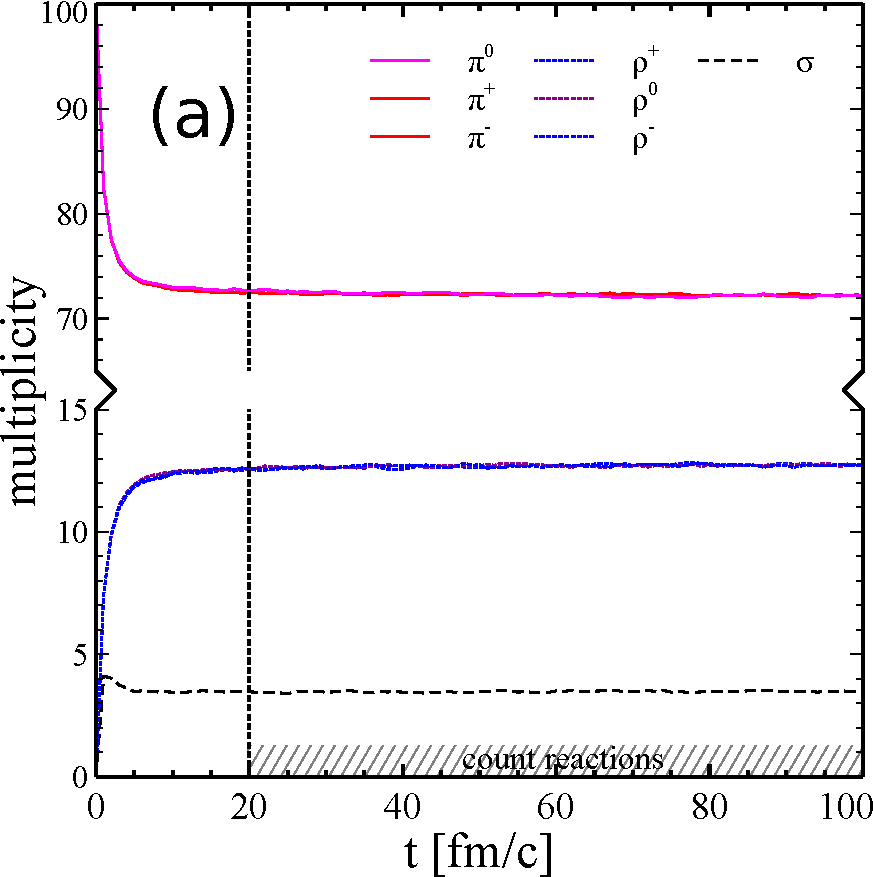
\includegraphics[height=6.5cm]{plots/smash/detailed_balance/rho_pi_sigma1.pdf}
  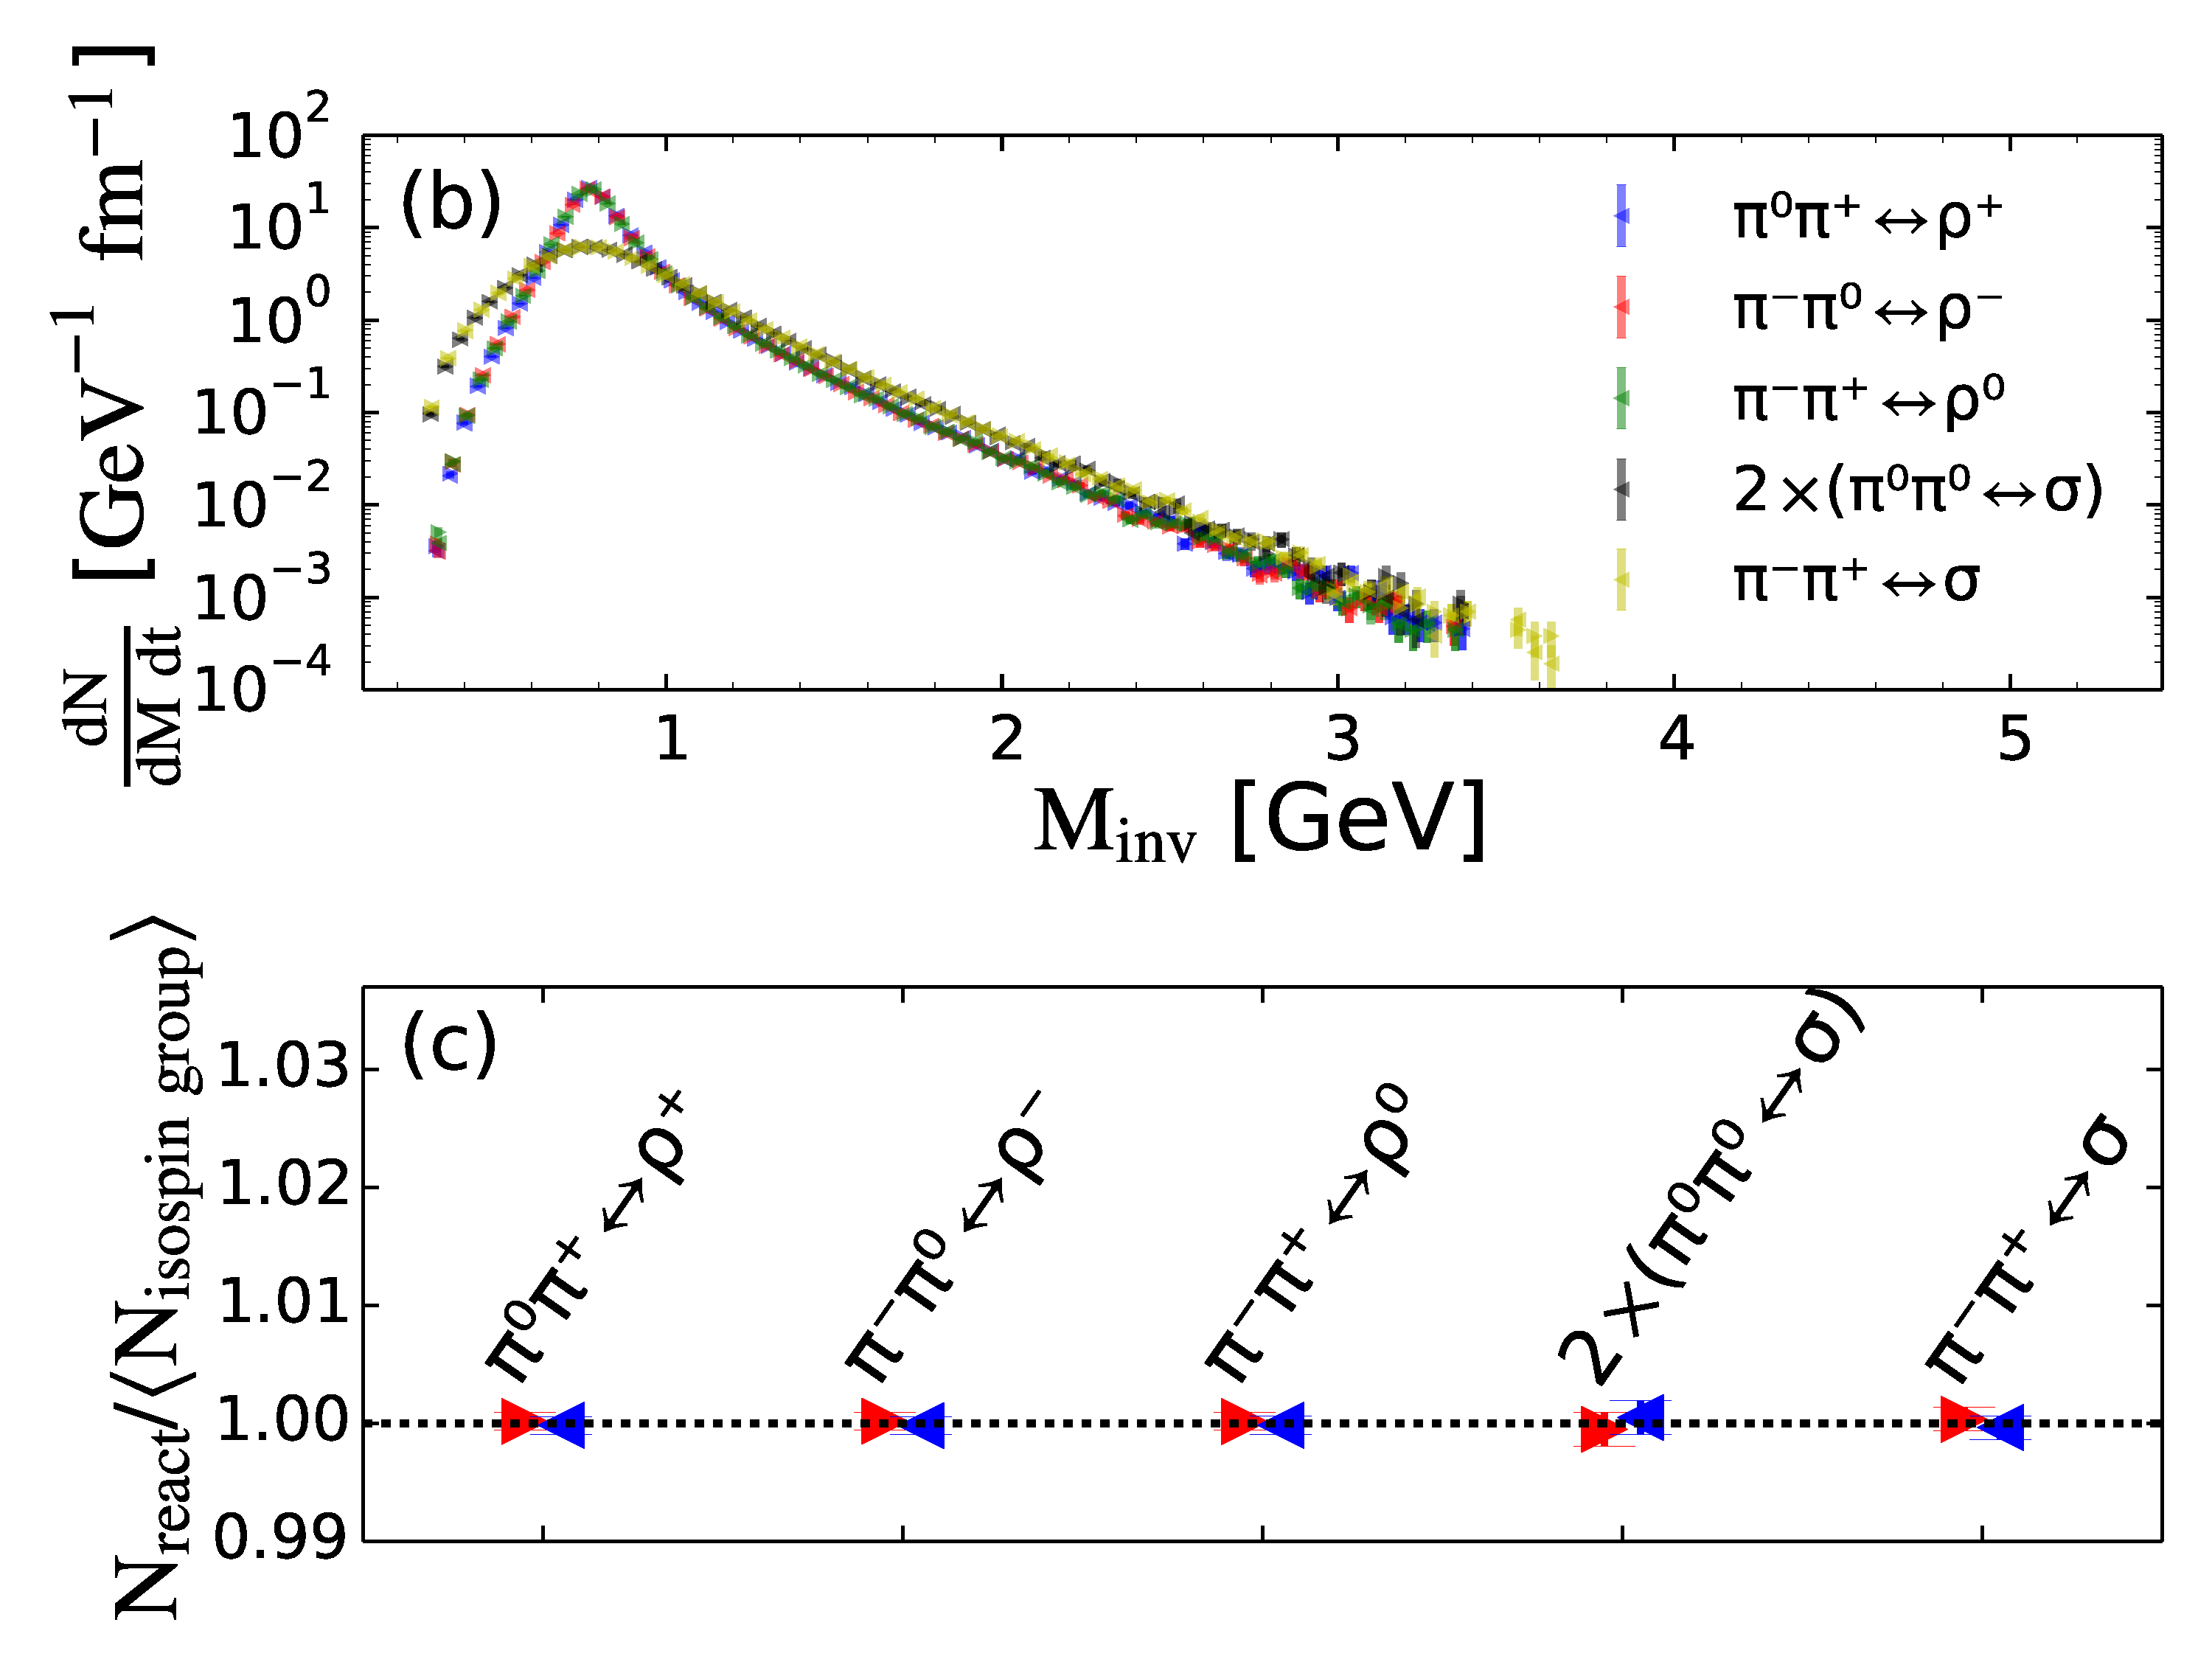
\includegraphics[height=6.5cm]{plots/smash/detailed_balance/react_num.pdf}
  \caption{Test of the detailed balance for the $\pi$-$\rho$-$\sigma$ system in a box
           with periodic boundary conditions. Multiplicities versus time (a), scaled
           numbers of forward and backward reactions for $t>20$ fm/c (c), and the same
           differentially versus the invariant mass of the reaction, which is equal to
           the resonance mass in this case (b).} \label{fig:pi_rho_sig_box}
\end{figure*}

In section~\ref{sec:det_bal} it was shown that from the time reversal
symmetry of elementary interactions it follows that matrix elements of forward
and reverse reactions are identical and in thermal equilibrium forward and
reverse reaction rates should be equal. In SMASH cross-sections are implemented
in such a way that the detailed balance principle is respected: if there is a
forward reaction then the reverse one is always implemented and the
cross-sections satisfy the detailed balance relations given in the
section~\ref{sec:det_bal}.

To test, if detailed balance actually holds in the calculations, a periodic
box was initialized with multiple particle species. After the matter reaches
equilibrium, it was verified that the rates of forward and backward reactions
are identical within statistical errors. The fact that the box should reach
equilibrium is granted by the H-theorem, which is derived assuming time
reversal invariance and the hypothesis of molecular chaos (Eq.
\ref{eq:molecular_chaos}). Strictly speaking, in a transport code both assumptions
are valid only in the limit $N_\text{test} \to \infty$. At finite
$N_\text{test}$ the interactions are non-local due to the geometrical cross
sections.  In addition, while two particles with space coordinates $\vec{r}_1$
and $\vec{r}_2$ form a resonance at $(\vec{r}_1 + \vec{r}_2)/2$, the products
of resonance decay obtain the same position as the decaying resonance. This
breaks the time reversal invariance and may lead to a small violation of
detailed balance, which vanishes at large $N_\text{test}$. This is indeed what
occurs, as it is shown further.

For the test two configurations were used: a $\rho-\pi-\sigma$ box and a
$N-\pi-\Delta$ box. The first one was initialized with a 100 $\pi^+$, 100
$\pi^-$ and 100 $\pi^0$ in a volume of $V = (10$ fm$)^3$. The reactions $\pi\pi
\leftrightarrow \rho$ and $\pi\pi \leftrightarrow \sigma$ were allowed, while
all the other possible reactions were switched off. From
Fig. \ref{fig:pi_rho_sig_box} one observes that the system has reached chemical
equilibrium, since the particle multiplicities in the box have saturated after around
$t=20$ fm/c. Starting from this time, forward and backward reactions were
counted. The matrix elements of reactions in the same isospin group differ only
by Clebsch-Gordan coefficients. Thus one expects, for example, that the number
of reactions $N(\sigma \leftrightarrow \pi^+ \pi^-) = 2 N(\sigma
\leftrightarrow \pi^0 \pi^0)$. Therefore, the reaction numbers in
Fig.~\ref{fig:pi_rho_sig_box} were scaled by the isospin and symmetry factors
appropriately to make sure that this expectation is fulfilled.  Detailed
balance is valid not only for the total number of reactions, but it also has to
be fulfilled differentially in momentum space. It is demonstrated in
Fig. \ref{fig:pi_rho_sig_box} that detailed balance is indeed fulfilled
differentially in each invariant mass bin of the reaction.  Note that
for the $\rho-\pi-\sigma$ box detailed balance for the total (but not
differential) number of reactions follows trivially from the multiplicity
saturation.

However, this is not the case for the $N-\pi-\Delta$ system. The $N-\pi-\Delta$ box was
initialized with 100 neutrons and 100 protons. The reactions $\Delta
\leftrightarrow N\pi$, $NN \leftrightarrow N\Delta$ and $NN
\leftrightarrow \Delta \Delta$ were allowed, with all the other reactions
being forbidden. As demonstrated in Fig. \ref{fig:pi_N_D_reactions} for
$N_\text{test} = 100$ detailed balance is violated at maximum by 2\%. For
$N_\text{test} = 1$ this violation can reach 10\% presumably because of the
non-locality effect described above.

To see if the numbers of reactions within one isospin group relate as expected
from Clebsch-Gordan factors, every number of reactions $N_i$ is multiplied by a
factor $\alpha_i$ that compensates for the isospin factors of this reaction.
Let us denote $\langle N_\text{isospin group} \rangle = \frac{1}{k}
\sum_{i=1}^k \alpha_i N_i$, where $k$ is amount of reactions in the isospin
group (forward + backward). If the SMASH result corresponds to the theoretical
expectation, then $N_i/\langle N_\text{isospin group} \rangle$ should be
strictly 1 for every reaction. One can extract from Fig. \ref{fig:pi_rho_sig_box}
and from Fig. \ref{fig:pi_N_D_reactions} that SMASH matches this expectation.
Table \ref{tab:clebsch} shows the origin of compensating coefficients $\alpha_i$.
While most of the Clebsch-Gordan factors are simple, for $pn \leftrightarrow
\Delta\Delta$ reactions they are less intuitive. The matrix element for $NN
\leftrightarrow \Delta\Delta$ reaction is isospin dependent, namely $|M(I=0)|^2
= \kappa |M(I=1)|^2$, where $\kappa = \frac{8}{3}$. Here is one explicit
example illustrating the calculation (where states beyond $I=1$ have been
omitted, since they drop out):

\begin{align}
  &|pn\rangle &=& \sqrt{\frac{1}{2}} | I=1 \rangle + \sqrt{\frac{1}{2}} | I=0 \rangle \\
  &|\Delta^- \Delta^{++} \rangle &=& \dots + \sqrt{\frac{9}{20}} | I=1 \rangle -
                                   \sqrt{\frac{1}{4}} | I=0 \rangle \\
  &\langle pn | \Delta^- \Delta^{++} \rangle ^2 &=& \frac{9}{40} |M(I=1)|^2 +
                                   \frac{5}{40} |M(I=0)|^2  \\
  &\langle pn | \Delta^- \Delta^{++} \rangle ^2 &=& \frac{5\kappa +9}{40} |M(I=1)|^2
\end{align}

Therefore, the detailed balance in SMASH for a mesonic system and a more
complex situation involving baryons and mesons is fulfilled.

\begin{figure*}
  %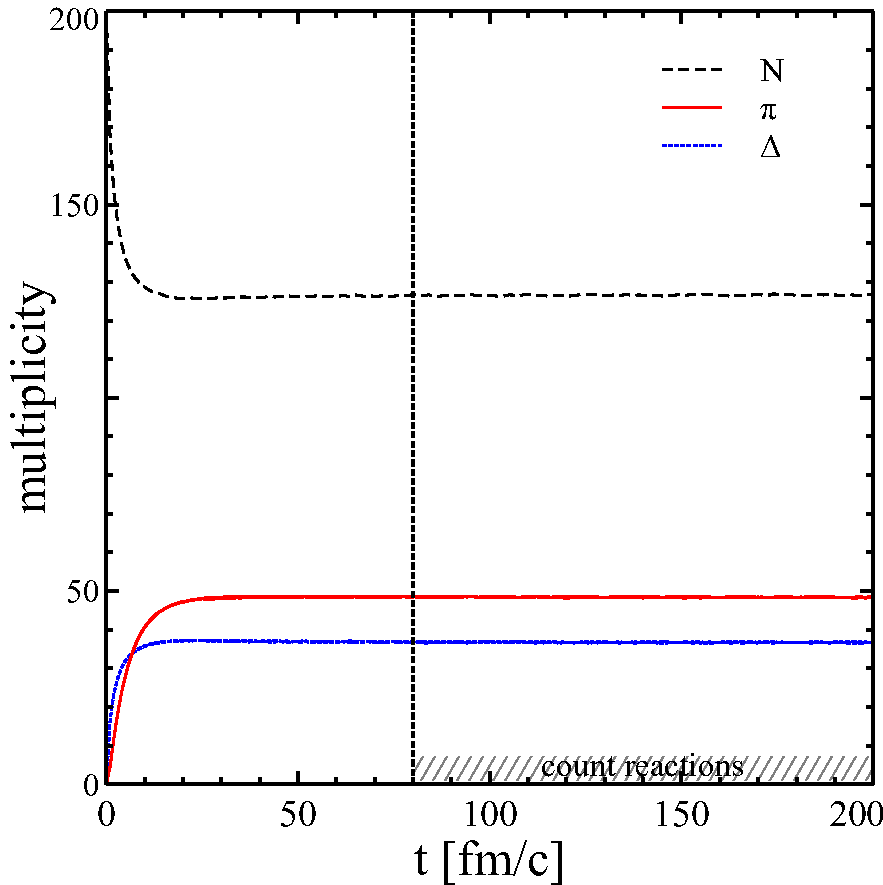
\includegraphics[width=0.48\textwidth]{plots/smash/detailed_balance/N_pi_Delta_mult.pdf}
  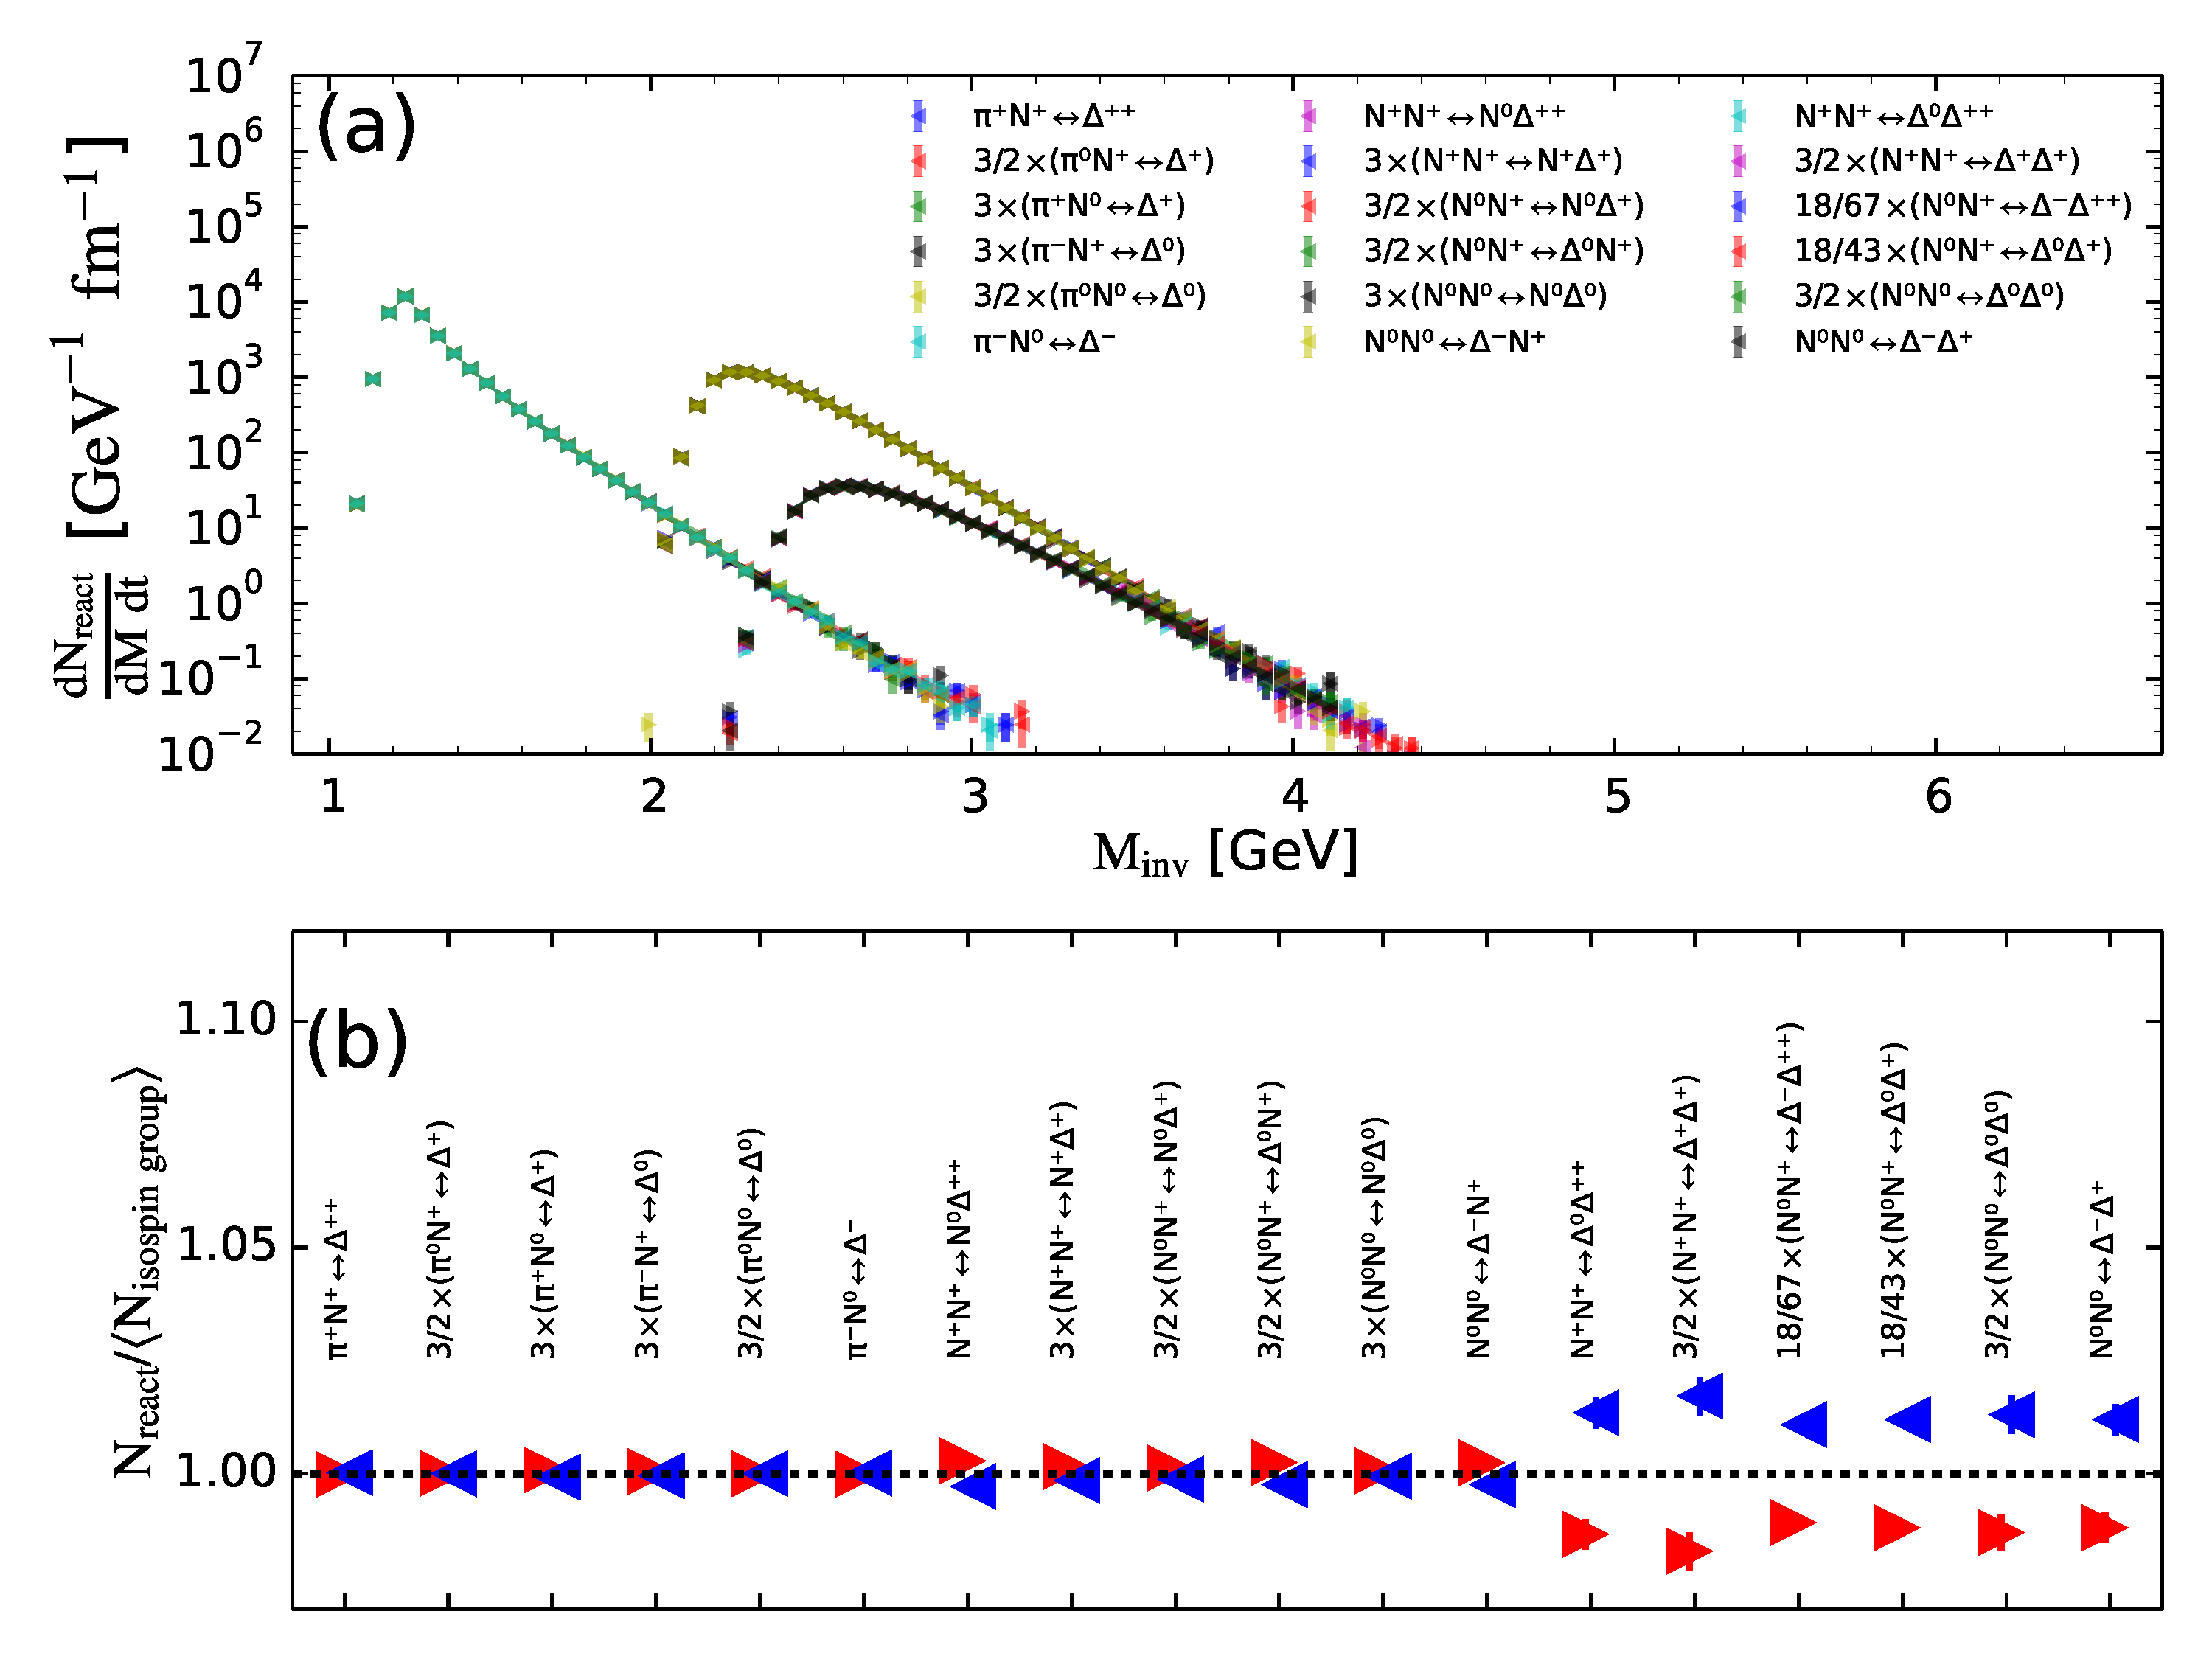
\includegraphics[width=\textwidth]{plots/smash/detailed_balance/react.pdf}
  \caption{Scaled numbers of forward (triangles right) and backward (triangles left)
           reactions for $t>80$ fm/c $\pi$-$N$-$\Delta$ (b) and the same differentially
           in the invariant mass of reaction (a).}
  \label{fig:pi_N_D_reactions}
\end{figure*}

\begin{table}
\begin{tabular}{cccc}
  \toprule
  Reaction                           &   Clebsch       &  Symmetry  &   Total \\
  \midrule
  $\rho^+\to\pi^+\pi^0$              &  $      1/2$  &     1      &   1/2     \\
  $\rho^-\to\pi^-\pi^0$              &  $      1/2$  &     1      &   1/2     \\
  $\rho^0\to\pi^0\pi^0$              &          $0$  &   1/2      &   0       \\
  $\rho^0\to\pi^+\pi^-$              &  $      1/2$  &     1      &   1/2     \\
  \midrule
  $\sigma\to\pi^+\pi^-$              &  $      1/3$  &     1      &   2/6     \\
  $\sigma\to\pi^0\pi^0$              &  $      1/3$  &   1/2      &   1/6     \\
  \midrule
  $p\pi^+\to\Delta^{++}$             &          $1$  &     1      &   3/3     \\
  $p\pi^0\to\Delta^{+}$              &  $      2/3$  &     1      &   2/3     \\
  $p\pi^-\to\Delta^{0}$              &  $      1/3$  &     1      &   1/3     \\
  $n\pi^+\to\Delta^{+}$              &  $      1/3$  &     1      &   1/3     \\
  $n\pi^0\to\Delta^{0}$              &  $      2/3$  &     1      &   2/3     \\
  $n\pi^-\to\Delta^{-}$              &          $1$  &     1      &   3/3     \\
  \midrule
  $pp\to p\Delta^{+}$                &  $      1/4$  &   1/2      &  1/8      \\
  $pp\to n\Delta^{++}$               &  $      3/4$  &   1/2      &  3/8      \\
  $pn\to n\Delta^{+}$                &  $      1/4$  &     1      &  2/8      \\
  $pn\to p\Delta^{0}$                &  $      1/4$  &     1      &  2/8      \\
  $nn\to p\Delta^{-}$                &  $      3/4$  &   1/2      &  3/8      \\
  $nn\to n\Delta^{0}$                &  $      1/4$  &   1/2      &  1/8      \\
  \midrule
  $pp\to\Delta^{0}\Delta^{++}$       &  $      6/20$ &   1/2      &  18/120   \\
  $pp\to\Delta^{+}\Delta^{+}$        &  $      8/20$ &   1/4      &  12/120   \\
  $pn\to\Delta^{-}\Delta^{++}$       &  $    67/120$ &     1      &  67/120   \\
  $pn\to\Delta^{+}\Delta^{0}$        &  $    43/120$ &     1      &  43/120   \\
  $nn\to\Delta^{+}\Delta^{-}$        &  $      6/20$ &   1/2      &  18/120   \\
  $nn\to\Delta^{0}\Delta^{0}$        &  $      8/20$ &   1/4      &  12/120   \\
  \bottomrule
\end{tabular}
  \caption{Expected isospin and symmetry factors for number of reactions within
           isospin groups at equilibrium. The first numeric column is a Clebsch-Gordan
           factor, the second column is symmetry factor, the third one is their product.}
\label{tab:clebsch}
\end{table}



\subsection{Potentials} \label{sec:potentials}

To create a more realistic simulation at low beam energies, a minimal version
of mean-field potentials between nucleons is included in the BUU way (see
section \ref{sec:transport}), i.e. with potentials dependent on local density
rather than distances between particles. The equations of motions follow from the
one-particle Hamiltonian $H_i$

\begin{equation}
  H_i = \sqrt{\vec p_i^{\,2} + m_{\textrm eff}^2} + U(\vec r_i)\,,
\end{equation}

where $m_{\textrm eff}$ is the mass for stable hadrons and the effective mass for
resonances in accordance with their mass distribution (e.g. Breit-Wigner). At
this point, the potential depends only on the coordinates, but not on the
momentum of the particles. The corresponding equations of motion are then

\begin{align}
  \frac{d\vec r_i}{dt} &=  \frac{\partial H_i}{\partial \vec p_i} =
         \frac{\vec p_i}{\sqrt{\vec p_i^{\,2} + m_{\textrm eff}^2}} \; , \\
  \frac{d\vec p_i}{dt} &= -\frac{\partial H_i}{\partial \vec r_i} =
        -\frac{\partial U}{\partial \vec r_i} \; .
\end{align}

In this formulation, as in any BUU approach, momentum conservation is fulfilled
only on average. Event by event momentum conservation requires that $d\vec
p_i/dt =-\partial H_\text{tot}/\partial \vec r_i$, where $H_\text{tot} = \sum_i
H_i$. The potential is calculated as a function of the local density

\begin{equation} \label{eq:potential}
  U = a (\rho/\rho_0) + b (\rho/\rho_0)^{\tau} \pm 2 S_\text{pot} \frac{\rho_{I3}}{\rho_0}
\end{equation}

Here $\rho$ is the Eckart rest frame baryon density and $\rho_{I3}$ is the
Eckart rest frame baryon isospin density of the relative isospin projection
$I_3/I$. The density calculation is described in section
\ref{sec:thermodynamics}. $\rho_0=0.168 1/\text{fm}^3$ is the nuclear
ground state density.  Parameters for the Skyrme potential are by default set
to $a=-209.2$ MeV, $b=156.4$ MeV and $\tau = 1.35$, while $S_\text{pot} = 18$
MeV is the default value for the symmetry potential. These parameters were
agreed on for a recent transport code comparison \cite{Xu:2016lue} and
correspond to a rather soft potential with an incompressibility of $K=240$ MeV.
For the equations of motion one does not need the potential itself, but its
gradient, $\partial U/\partial \vec r$. In the symmetry term the positive sign
is applied for the potential acting on neutrons and the minus sign is applied
for the potential acting on protons. Currently, the potential acts only on
baryons. The potentials are always calculated after the actions are performed,
right when the propagation happens.

Note that electromagnetic potentials (Coulomb and Lorentz force) are
currently being neglected in the model, since they are typically much weaker
than the hadronic mean fields (even if they are more long-ranged). The Coulomb
potential can only play a role for collisions of large nuclei at very low
energies and is completely negligible at higher energies (FAIR/RHIC/LHC).

\begin{figure}
  \centering
  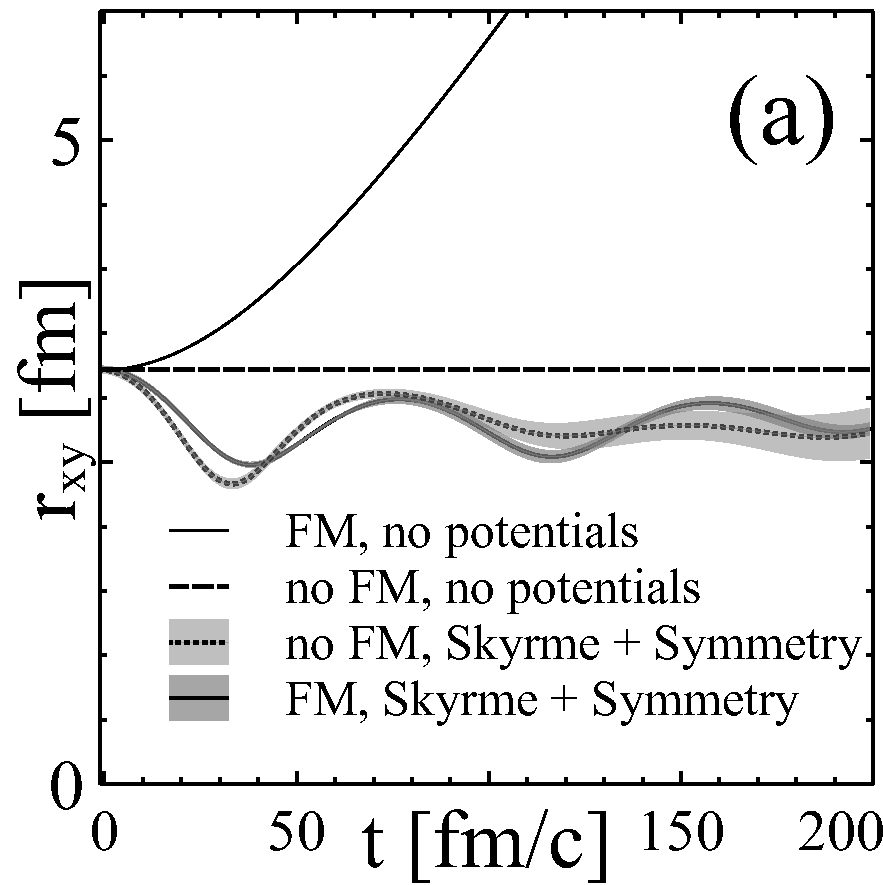
\includegraphics[width=0.49\textwidth]{plots/smash/Cu_nucleus_stability.pdf}
  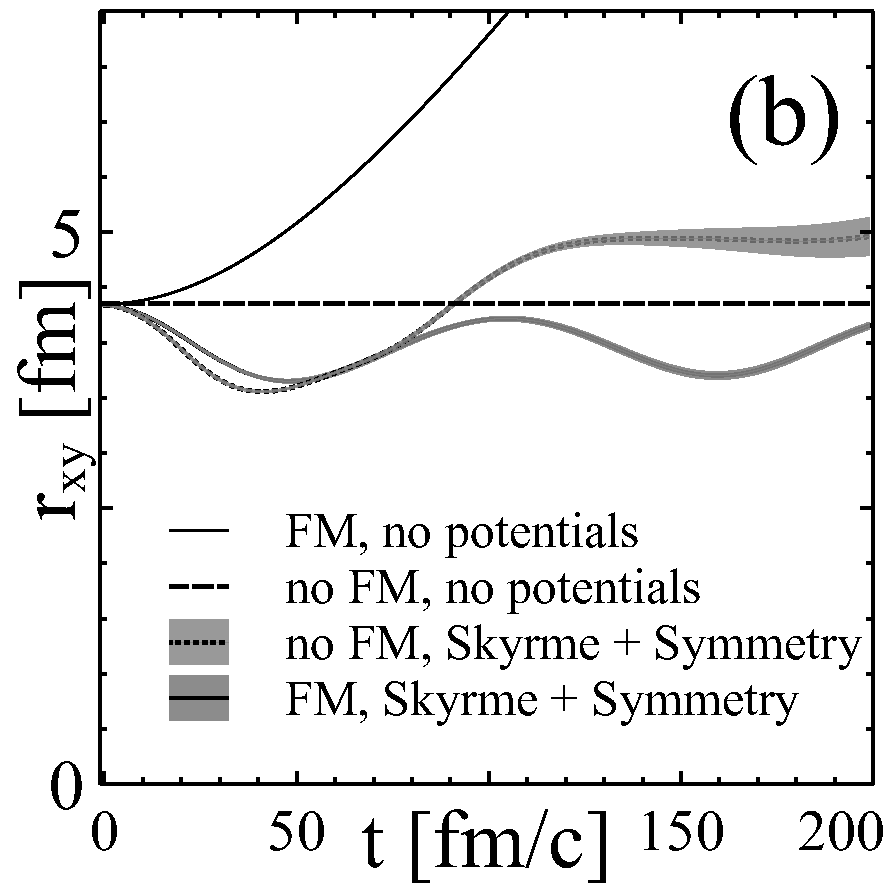
\includegraphics[width=0.49\textwidth]{plots/smash/Au_nucleus_stability.pdf}
  \caption{Evolution of an average transverse radius $r_{xy} = \sqrt{\langle x^2
           + y^2 \rangle}$ of a nucleus over 200 fm/c with different combinations of Fermi
           motion (FM) and potentials, $^{29}$Cu nucleus (a) and $^{79}$Au nucleus (b).}
  \label{fig:stability}
\end{figure}

Fig. \ref{fig:stability} shows the nuclear stability over a large time range,
much larger than what is actually relevant for a nucleus-nucleus collision. The
nucleons fly apart as expected, if only Fermi motion without potentials to
stabilize the nucleus are included. With potentials there is the expected
oscillatory behavior: The nucleons drift apart due to Fermi motion and the
potentials counteract and push them closer together again. One can also
observe the oscillations of the nucleus during the propagation. This can be avoided
if the nucleus is initialized in its ground state~\cite{Gaitanos:2010fd}.
The observed oscillations are called a giant monopole resonance or a
''breathing mode'' of the nucleus.

Computations with potentials require that time step is small enough - the
energy change per timestep should be much smaller than the energy of the
particle:

\begin{equation}
  \frac{\Delta E}{E} \simeq \frac{|\partial U/ \partial r| \Delta t}{E} \ll 1 \,.
\end{equation}

\subsection{Pauli blocking}

Pauli blocking is an effective way to obtain the solution of the quantum BUU
equation, Eqs. (\ref{eq:buu_icoll}-\ref{eq:Boltz}), from classical molecular
dynamics. Indeed, the BUU equations differ from the Boltzmann equations only by $(1
\pm \mathit{f})$ factors in the collision integral. Here the plus sign is for
bosons and the minus sign for fermions. One can interpret these factors as a
multiplication of the cross sections by $\prod_i (1 \pm f_i)$, where the
product is taken over all final states in the reaction and $f_i \equiv
f(r_i,p_i,t)$ is the phase-space density of final-state particle $i$. This
means that for bosons cross sections are effectively increased and for fermions
cross sections are effectively decreased. This is called Bose enhancement and
Pauli-blocking respectively. While Bose enhancement has been attempted to
implement recently in a parton cascade \cite{Xu:2014ega}, Pauli blocking is
taken into account in many transport approaches. It is known to be especially
important at low collision energies.

The implementation of Pauli blocking consists of two parts: the calculation of
the phase-space density and the rejection of reactions with probability $1 -
\prod_i (1-f_i)$. For the latter SMASH loops over all baryons in the final
state after a collision has taken place and returns 'true' for blocking, if a
uniformly distributed random number $r > f_i$. This means that the reaction is
not blocked with probability $\prod_i (1-f_i)$. In this way, no fermion should be
produced or scatter into a phase space bin that is already occupied by another
fermion.

The implementation of the phase space density calculation basically follows the
method used in the GiBUU model, see section D.4.3 in \cite{Buss:2011mx}. By
definition $N(\Delta V_r, \Delta V_p) = g f(r,p) \Delta V_r  \Delta V_p$, where
$N$ is the number of (test)particles in a given phase-space volume $\Delta V_r
\Delta V_p$ and $g$ is the degeneracy. Theoretically, the size of the
phase-space goes to zero $\Delta V_r, \Delta V_p \to 0$. In practice $\Delta
V_r$, $\Delta V_p$ and the way of averaging are chosen to balance between the
smoothness of the obtained distribution function and the resolution of
coordinate and momentum space. This implementation relies on a large number of
test particles ($\Ntest > 20$).

The phase-space density is calculated according to the following equations:

\begin{align}
  f_i (r_j,p) &= \sum_{j: p_j \in V_p} \frac{1}{\kappa (2 \pi \sigma^2)^{3/2}}
            \int_{\Delta V_r, |r - r_j| < r_c} d^3r \, \nonumber\\
            &\times \exp \left( - \frac{(r-r_j)^2}{2 \sigma^2} \right)
\end{align}

with $\kappa$ given as

\begin{align}
  \kappa &= \frac{2 \Delta V_r \Delta V_p N}{(2 \pi)^3} \frac{4 \pi}{(2 \pi \sigma^2)^{3/2}}
        \int_0^{r_c} dr \, \nonumber\\
       &\times r^2 \exp \left(- \frac{r^2}{2 \sigma^2}\right)
\end{align}

\begin{figure}
  \centering
  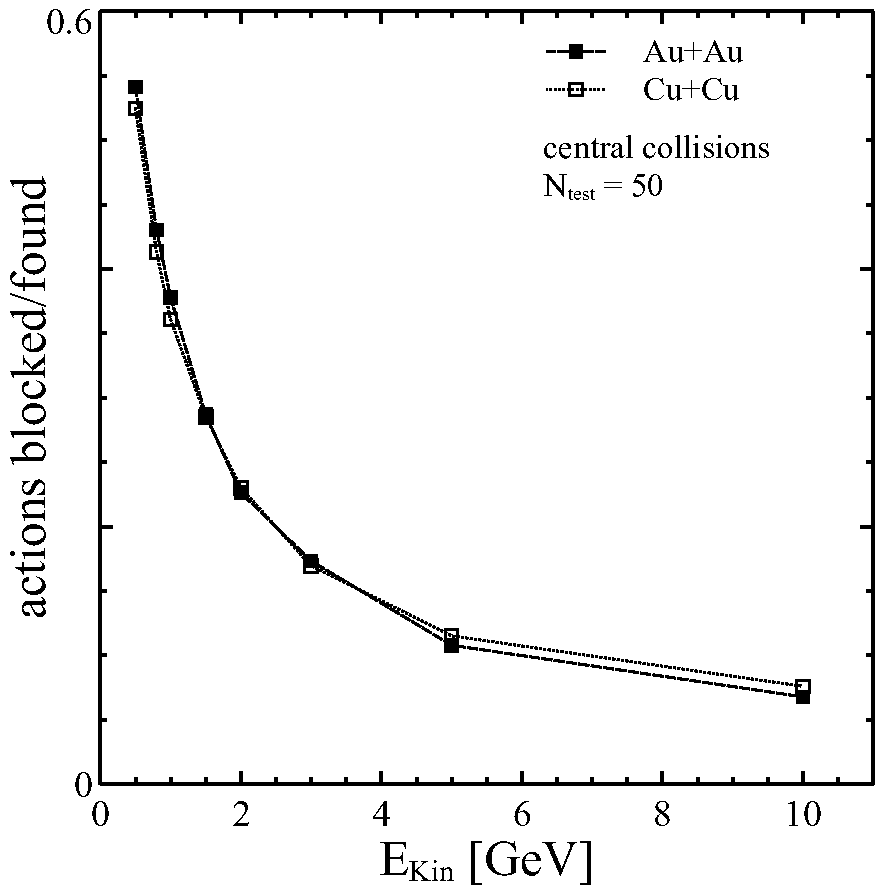
\includegraphics[width=0.48\textwidth]{plots/smash/PB_ekin.pdf}
  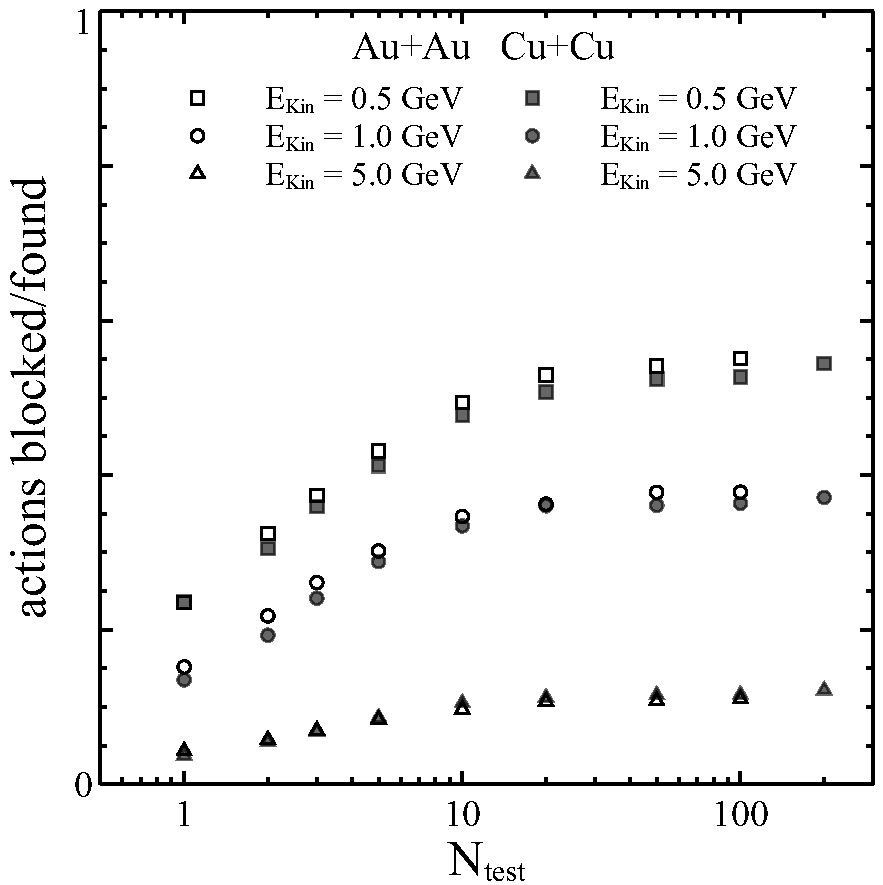
\includegraphics[width=0.48\textwidth]{plots/smash/PB_ntest.pdf}

  \caption{Left panel: Ratio of Pauli blocked to total found actions in Cu+Cu and Au+Au
           collisions at different beam energies. For reference, the total number of found
           actions per event (both blocked and performed) in an Au+Au collision at
           $E_\text{kin} = 0.5A\,\text{GeV}$ is $0.99 \cdot 10^5$, for $E_\text{kin} =
           5A\,\text{GeV}$ it constitutes $1.32 \cdot 10^5$. The number of test particles
           used in the simulation is $N_\text{test} = 50$.
           Right panel: Ratio of Pauli blocked to total found actions in Cu+Cu (filled
           symbols) and Au+Au (open symbols) collisions for different numbers of test
           particles.}
  \label{fig:pauli_blocking}
\end{figure}

Here $\vec{r}_j$ is a vector connecting the point, where $f$ is calculated, and
the position of the $j$-th particle. All these expressions can be analytically
further evaluated for $r_c>r_r$. This is a reasonable assumption, because the
Gaussian cut-off $r_c$ has to be large enough, so that the results do not
depend on it. If $r_c<r_r$ the whole method is hardly applicable. In GiBUU
these integrals are computed numerically, but analytical expressions for them
also exist (see appendix of \cite{Weil:2016zrk}). For $V_p$ a sphere of radius 80 MeV
is taken.

\begin{figure}
  \centering
  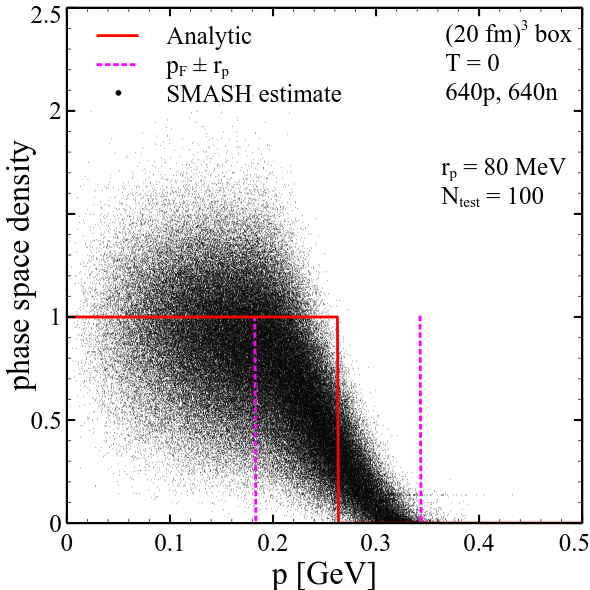
\includegraphics[width=0.5\textwidth]{plots/smash/SMASH_testsetup_ntest100_rp80.png}
  \caption{Estimated distribution function at collision points is compared to
           analytical one. Periodic (20 fm)$^3$ box filled with 640 protons
           and 640 neutrons that are only allowed to collide elastically.
           The initial distribution is Fermi-Dirac distribution at zero temperature,
           so all the collisions should ideally be blocked.}
  \label{fig:f_estimate}
\end{figure}

In Fig. \ref{fig:pauli_blocking} the number of collisions that is blocked due
to prior phase space occupation has been calculated in central Cu+Cu and Au+Au
collisions as a function of beam energy. One can see that at very low energies
there are as many blocked collisions compared to collisions taking place. The ratio
drops rather fast and around $E_{\textrm kin} = 2A$ GeV only a quarter of the
collisions are blocked. It then saturates around 10\% for higher beam energies.

The right panel of Fig. \ref{fig:pauli_blocking} demonstrates the need for a
decent number of test particles to obtain stable results. If the number of test
particles is low the phase-space volume cannot be calculated with enough
precision and therefore, there are too many collisions allowed. Saturation sets
in around $N_{\textrm test} =20$ and is very similar for Au+Au and Cu+Cu
collisions.

One can notice from Fig. \ref{fig:pauli_blocking} that even for a very large
number of testparticles there are collisions inside the nucleus, which should
never happen in nature.  To demonstrate how these collisions occur, a box with
periodic boundaries is initialized with Fermi-Dirac distribution at zero
temperature. In this case no collisions should be allowed, because analytically
$\mathit{f} = 1$. The estimated values of the phase-space density $\mathit{f}$
are shown in Fig. \ref{fig:f_estimate}. The estimation of the phase-space
density employs smearing, so the sharp boundary in momentum space is smeared
and $\mathit{f}$ is underestimated for $p < p_F$ and overestimated for $p <
p_F$. This effect is significant within the momentum smearing radius $|p - p_F|
< r_p$.  For low momenta \emph{in average} $\mathit{f}$ is estimated correctly,
but any underestimation in particular events unavoidably causes unwanted collisions.

Since collisions in the nucleus cannot be completely avoided using Pauli-blocking,
sooner or later the nucleus thermalizes due to these collisions. To avoid this unwanted effect
in SMASH collisions within a nucleus are explicitly forbidden unless the nucleon
has already collided with some external particle.


\section{Thermodynamics in the SMASH transport approach} \label{sec:thermodynamics}

\subsection{Thermodynamic quantities from coarse-grained SMASH}

\begin{figure}
  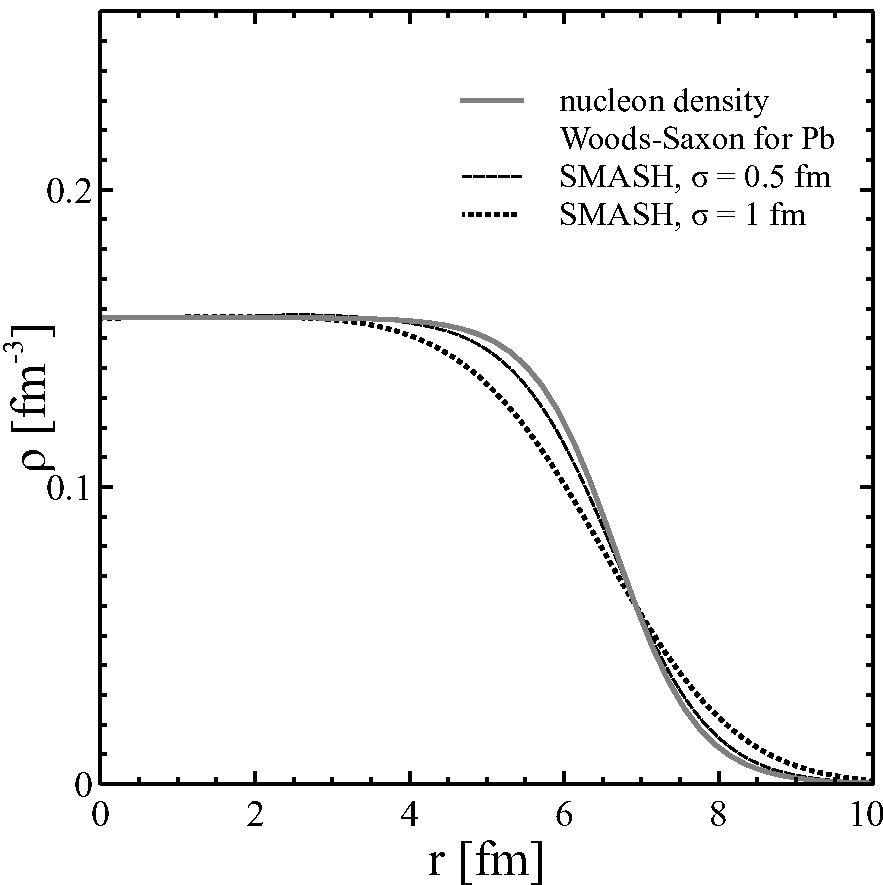
\includegraphics[width=0.5\textwidth]{plots/smash/thermodynamics/density_smearing.pdf}
  \caption{Baryon density estimated in SMASH simulation with smearing $\sigma =
           0.5$ fm (dashed line) and 1.0 fm (dotted line) is compared to the true density
           profile (solid line). Large $N_\text{test} = 1000$ for $\sigma = 1$ fm and
           $N_\text{test} = 10000$ for $\sigma = 0.5$ fm is taken to diminish
           fluctuations.}
  \label{fig:density:smear}
\end{figure}

Thermodynamic quantities such as net baryon density, total number density,
energy density, temperature, chemical potentials (baryon, strangeness, isospin, etc)
are necessary in several cases. Firstly, densities are used to compute potentials
 (see section \ref{sec:potentials}). Secondly, they are needed for the forced thermalization
(chapter \ref{chap:forced_therm}). Thirdly, thermodynamic quantities are very useful
to visualize heavy ion collisions, since they represent both coordinate and momentum
space in an intuitively simple way.


The first step to compute thermodynamic quantities is constructing four-currents
and energy-momentum tensor

\begin{align}
  T^{\mu\nu}(\vec{r}) &= \frac{1}{N_\text{ev} N_\text{test}} \sum_\text{events} \sum_i \frac{p^{\mu}_i p^{\nu}_i}{p^0_i} K(\vec{r} - \vec{r_i}, p_i)  \\
  j^{\mu}(\vec{r})    &= \frac{1}{N_\text{ev} N_\text{test}} \sum_\text{events} \sum_i \frac{p^{\mu}_i}{p^0_i} K(\vec{r} - \vec{r_i}, p_i) \,,
\label{eq:tmn_jmu}
\end{align}

where $N_\text{ev}$ is the number of events and $N_\text{test}$ is the test
particle number. The formulas were derived in section
\ref{sec:coarse_graining}, an explicit form of the used smearing kernel $K$
(Eq. \ref{eq:smearing_kernel}) is suggested and justified in the same section.
In the limit of the smearing width $\sigma \to 0$ and
$N_\text{ev}N_\text{test} \to \infty$ the full smooth quantities are obtained.
This limit is numerically challenging, because when reducing the smearing width
$\sigma$, one has to increase statistics, keeping $\sigma^3
N_\text{ev}N_\text{test}=\text{const}$. Therefore, one takes a reasonably small
$\sigma = 1$ fm and keeps in mind the smearing effect, which is demonstrated in
Fig. \ref{fig:density:smear} for the density calculation of a Pb nucleus comparing
$\sigma = 0.5$ fm and 1 fm.

The next step is to transform $\Tmn$ and $\jmu$ to a local rest frame. In principle,
there is a variety of possible rest frames, e.g. a frame of zero total/pion/baryon/etc
 momentum current; a frame of zero entropy current; a frame of zero total/baryon/electric/etc current;
center of momentum frame and so on. All these frames only coincide in the case of
ideal hydrodynamics. For a coarse-grained transport they are different in general.

\begin{figure}
  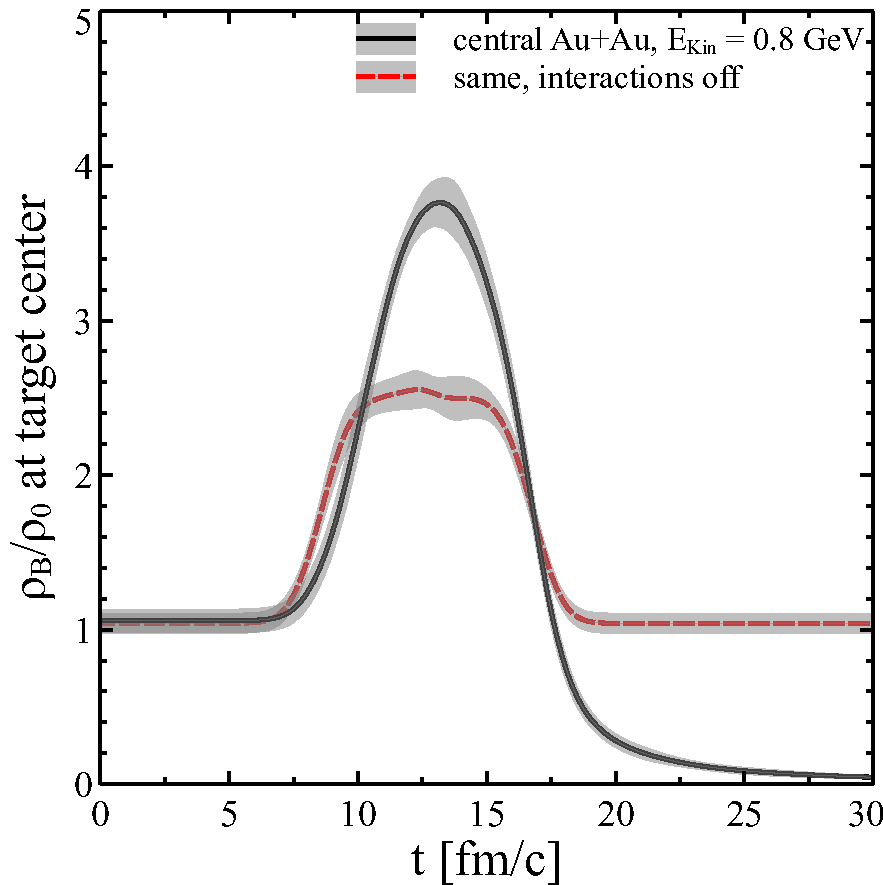
\includegraphics[width=0.49\textwidth]{plots/smash/thermodynamics/density_at_target_center_AuAu_Ekin08GeV_fixed_target.pdf}
  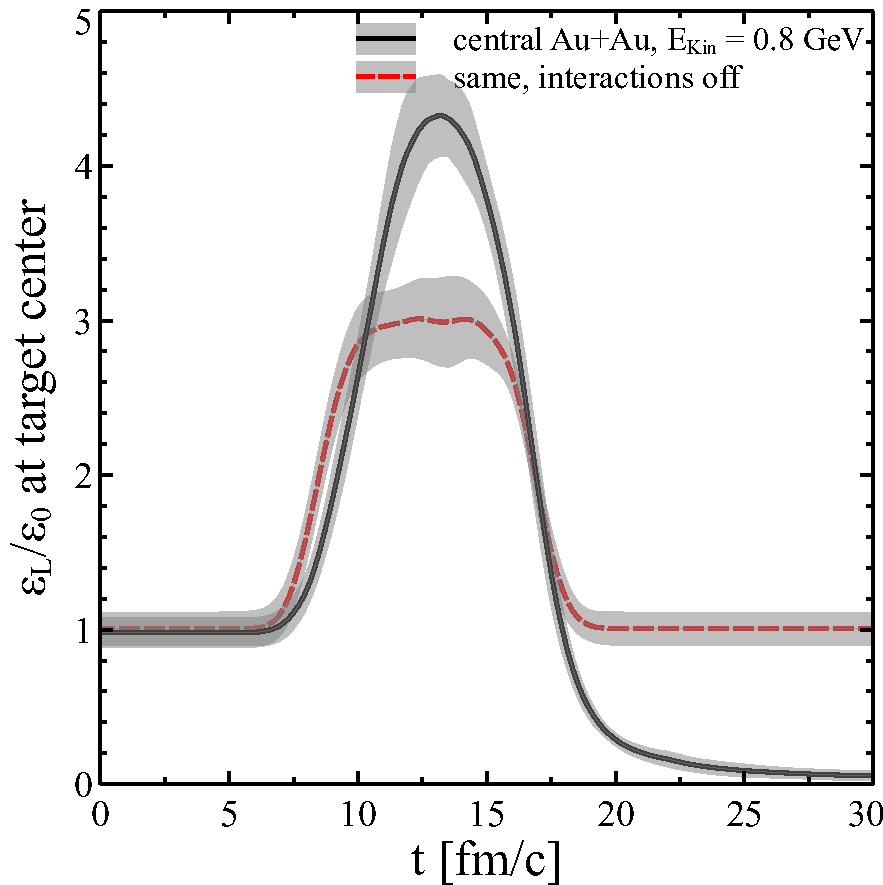
\includegraphics[width=0.49\textwidth]{plots/smash/thermodynamics/e_at_target_center_AuAu_Ekin08GeV_fixed_target.pdf}

  \caption{Eckart rest frame net baryon density $\rho_B$ (left panel) and
           Landau rest frame hadron density $\epsilon$ (right panel) at the
           target center in central Au+Au collision at $\Elab = 0.8$ \emph{A} GeV
           in units of the ground state nuclear density $\rho_0$ / ground state nuclear
           energy density $\epsilon_0 = 0.150$ GeV/fm$^3$. Simulation is performed in
           the fixed target frame. Time dependence for the full SMASH simulation (full
           line) is compared to the SMASH simulation with all interactions off (dashed
           line).}
  \label{fig:density:AuAu}
\end{figure}

SMASH uses three rest frames: Landau rest frame (zero total momentum current or
equivalently $T^{0i} = 0$ for $i = 1,2,3$), net baryon Eckart frame (zero
net baryon current of $j_B^{0i} = 0$ for $i = 1,2,3$) and net $\frac{I_3}{I}$
Eckart rest frame. The latter two are currently used to compute baryon density
and net $\frac{I_3}{I}$ density, which stand in the expression for potentials
 (Eq. \ref{eq:potential}).

Since $j^{\mu}j_{\mu}$ is relativistically invariant, the Eckart rest frame density
is obtained as $\rho_\text{Eck} =\sqrt{j^{\mu}j_{\mu}}$. For net baryon
(charge, isospin projection) density a naive weighting of particles in Eq.
(\ref{eq:tmn_jmu}) with their baryon numbers can give rise to $j^{\mu}j_{\mu}
<0$, meaning that Eckart frame is undefined. To avoid this, the density is
computed as $\rho = \rho^+ - \rho^-$, where~$+$ corresponds to positive baryon
number (charge, isospin projection) and~$-$ corresponds to negative ones. In
the left panel of Fig. \ref{fig:density:AuAu} the dependence of the net baryon
density versus time in the middle of the target in the central Au+Au collision
at $E_\text{kin} = 0.8A$ GeV in the fixed-target frame is shown. The energy
density in the Landau frame is depicted in the same figure on the right panel.
From these plots one can see that the ground state baryon/energy density values
are reproduced, when the collision term is disabled. Including interactions the
baryon/energy density rises to about 4 times the nuclear ground state
densities.

The Landau rest frame (LRF) quantities in SMASH are used for the forced
thermalization. The advantage of the Landau rest frame is that it is always
well-defined. By definition, $T^{0i}_\text{LRF} = 0$, the energy flow in the
LRF is zero. To find the LRF, one has to find such a Lorentz boost that after it
$T^{0i} = 0$. To achieve this the generalized eigenvalue problem

\begin{equation}
  (T^{\mu \nu} -\lambda g^{\mu \nu})h_{\nu} = 0
\end{equation}

is solved, where $g^{\mu \nu}$ is the metric tensor. The eigenvectors are
normalized so that $h^{\mu}h_{\mu} = 1$. Note that this generalized eigenvalue
problem is equivalent to a usual eigenvalue problem for $T^{\mu}_{\nu}$,
however $T^{\mu}_{\nu}$ is neither symmetric nor positively defined, so
numerical solvers look for complex eigenvalues. In contrast, the above
generalized eigenvalue decomposition of $\Tmn$ always gives real eigenvalues,
since it is symmetric and positively defined:

\begin{equation}
\Tmn = \Lambda^T diag(\lambda_{1-4}) \Lambda \,,
\end{equation}

where $\Lambda$ is a matrix consisting of eigenvectors $h_{\mu}$. Note that
this eigenvector decomposition is identical to the Lorentz transformation from
the rest frame, where the upper row of the boost matrix (Eq.
\ref{eq:lorentz_boost_matr}) is the required boost four-velocity $u^{\mu}$.
At the same time the upper row is one of the generalized eigenvectors $h^{\mu}$
of $\Tmn$. Therefore, to find the required boost one just has to choose the
right eigenvector from the four solutions of the eigenvalue problem.

Notice that the eigenvalue corresponding to $u^{\mu}$ is the LRF energy density
$\epsilon$, the rest of the eigenvalues of $T^{\mu}_{\nu}$ are non-positive and
smaller by magnitude. One can see this immediately assuming that
$T^{\mu}_{\nu}$ is computed from particles directly in the LRF.  Therefore, the
normalized eigenvector corresponding to the largest (and the only positive)
eigenvalue is the required 4-velocity of the LRF.

To demonstrate the result of this transformation the LRF energy density and
collective velocities $u^\mu$ are plotted in the $x$-$z$-plane in Fig.
\ref{fig:landau_e_v} for a Au+Au collision. One can observe the onset of radial
flow after the initial collision of the two nuclei. Note that the LRF energy
density before collision reproduces again the nuclear ground state energy
density.

\begin{figure*}
  \centering
  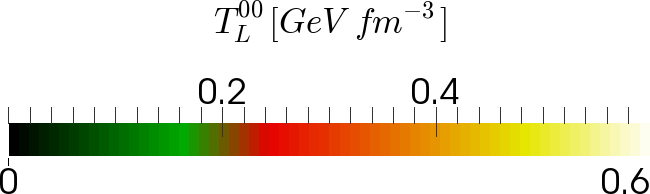
\includegraphics[width=0.35\textwidth]{plots/smash/thermodynamics/AuAu_EKin08GeV_b3_Ntest20/scale_T00.png}  \\
  \vspace{0.1cm}
  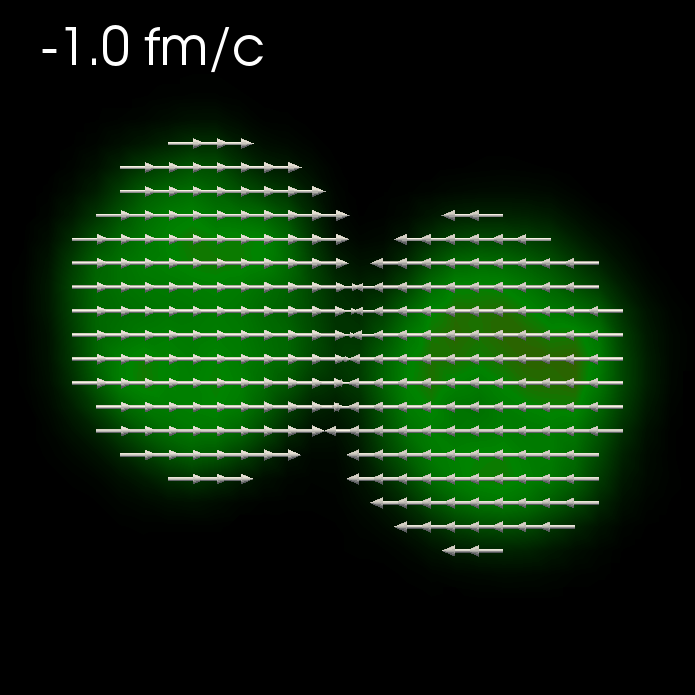
\includegraphics[width=0.3\textwidth]{plots/smash/thermodynamics/AuAu_EKin08GeV_b3_Ntest20/AuAu_EKin08_b3_1.png}
  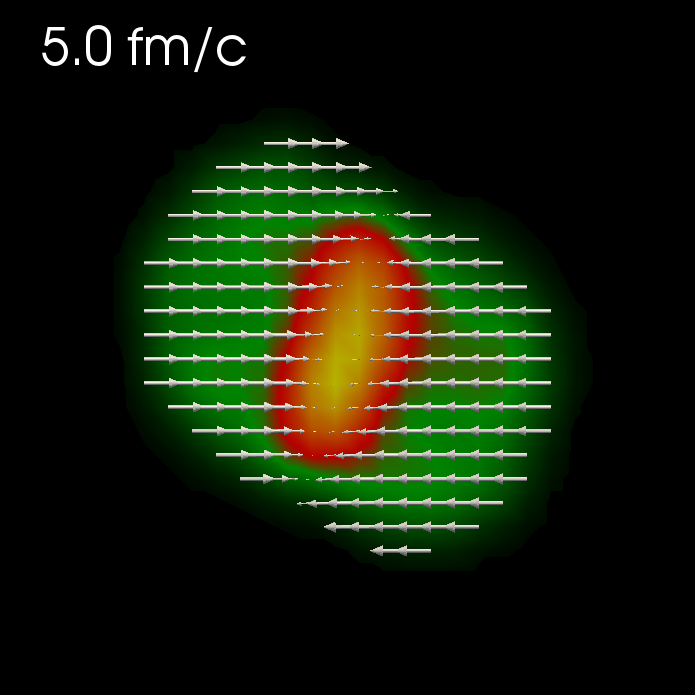
\includegraphics[width=0.3\textwidth]{plots/smash/thermodynamics/AuAu_EKin08GeV_b3_Ntest20/AuAu_EKin08_b3_2.png}
  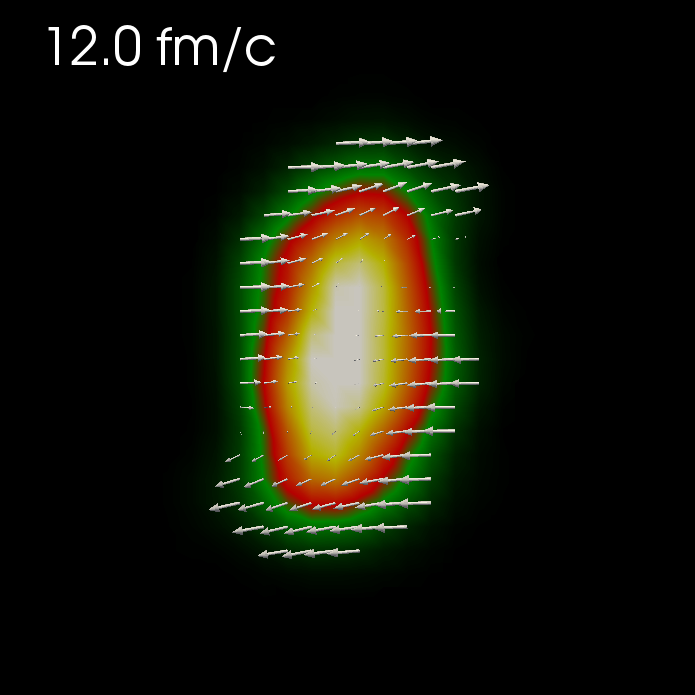
\includegraphics[width=0.3\textwidth]{plots/smash/thermodynamics/AuAu_EKin08GeV_b3_Ntest20/AuAu_EKin08_b3_3.png} \\
  \vspace{0.1cm}
  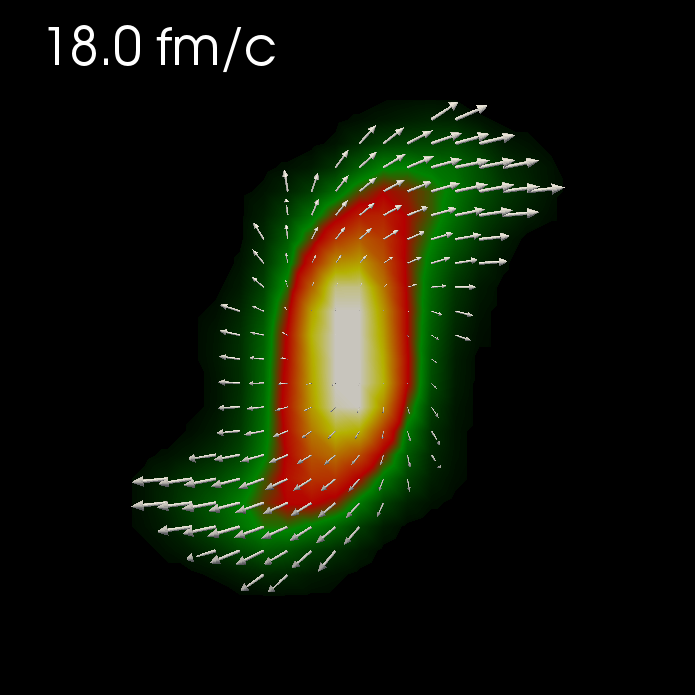
\includegraphics[width=0.3\textwidth]{plots/smash/thermodynamics/AuAu_EKin08GeV_b3_Ntest20/AuAu_EKin08_b3_4.png}
  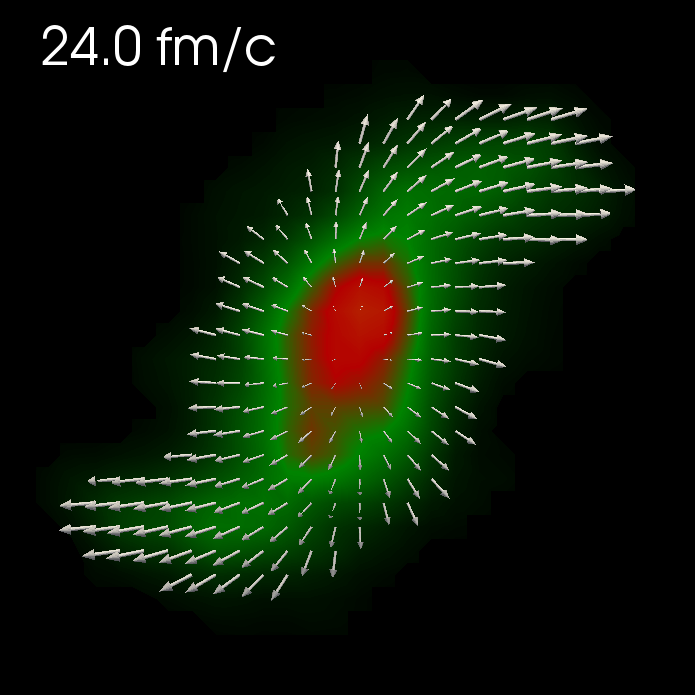
\includegraphics[width=0.3\textwidth]{plots/smash/thermodynamics/AuAu_EKin08GeV_b3_Ntest20/AuAu_EKin08_b3_5.png}
  \caption{ Landau rest frame energy density $T^{00}_L$ (background color) and
           velocity of Landau frame (arrows), both for baryons. Au+Au collision at
           $E_\text{kin} = 0.8A\,\text{GeV}$ with impact parameter $b = 3\,\text{fm}$,
           $N_\text{test} = 20$. Color legend is given above. Velocity is proportional
           to
           the arrow length, maximal arrow length corresponds to velocity of 0.55 $c$.  }
  \label{fig:landau_e_v}
\end{figure*}



\subsection{SMASH equation of state} \label{sec:smash_eos}

\begin{figure}
  \centering
  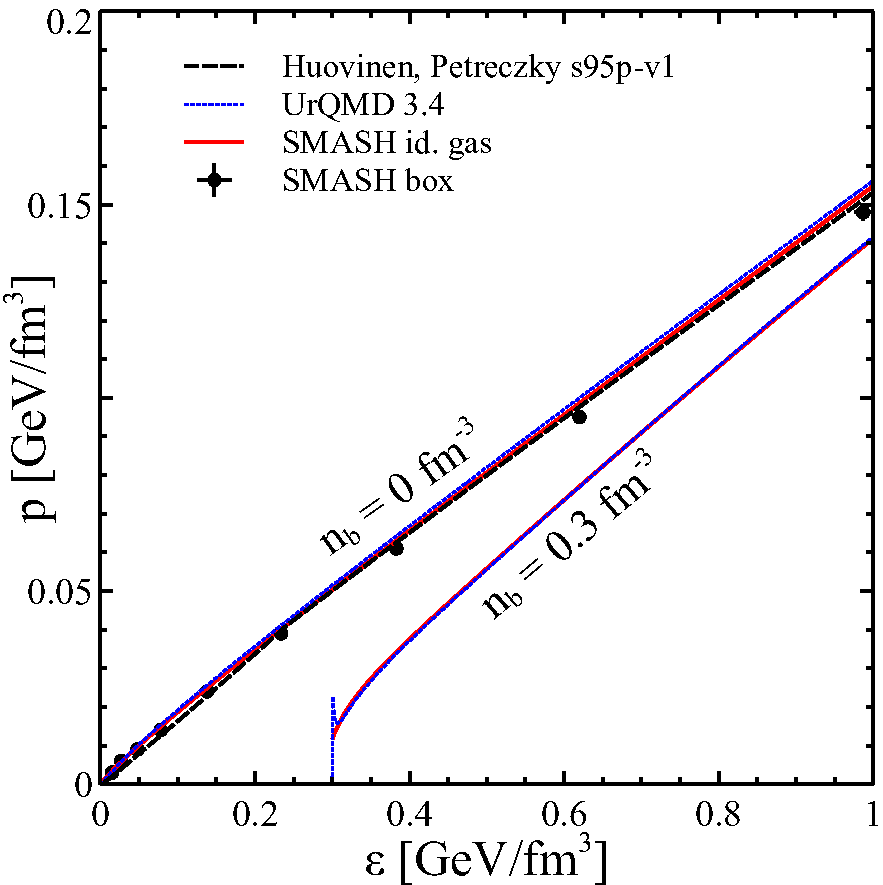
\includegraphics[width=0.5\textwidth]{plots/forced_thermalization/eos.pdf}
  \caption{Equation of State (EoS) comparison between ideal gas consisting of
           hadrons implemented in SMASH (solid lines), in UrQMD (dotted lines) and 
           s95p-v1 QCD EoS from \cite{Huovinen:2009yb} (dashed line).}
  \label{FIG:I}
\end{figure}

In Figure \ref{FIG:I} the equation of state arising from SMASH is compared to UrQMD
and to the parametrized lattice QCD equation of state from \cite{Huovinen:2009yb},
which is used in many hydrodynamical calculations. The SMASH EoS is computed in two
ways. First, the EoS of ideal gas consisting of all SMASH hadrons is calculated
according to Eqs. (\ref{eq:id_hadgas_eos1}-\ref{eq:id_hadgas_eos3}). This EoS does not
take the effects of resonance widths into account. It is compared to SMASH EoS
computed in a different way. A box with periodic boundary conditions is initialized
with a set of hadrons, their multiplicities being computed according to an ideal gas
EoS with pole masses. Then one waits for 1000 fm/c, until the mixture equilibrates (it
is checked the hadron multiplicities saturate over time) and computes
pressure and energy density. The results are plotted in Fig. \ref{FIG:I}: the SMASH
box EoS only slightly deviates from the naive ideal gas EoS. The effects of non-zero
widths tend to decrease pressure slightly at a given energy density.